%%
%% This is file `thesis.tex',
%% generated with the docstrip utility.
%%
%% The original source files were:
%%
%% nudtpaper.dtx  (with options: `thesis')
%% 
%% This is a generated file.
%% 
%% Copyright (C) 2012 by Liu Benyuan <liubenyuan@gmail.com>
%% 
%% This file may be distributed and/or modified under the
%% conditions of the LaTeX Project Public License, either version 1.3a
%% of this license or (at your option) any later version.
%% The latest version of this license is in:
%% 
%% http://www.latex-project.org/lppl.txt
%% 
%% and version 1.3a or later is part of all distributions of LaTeX
%% version 2004/10/01 or later.
%% 
%% To produce the documentation run the original source files ending with `.dtx'
%% through LaTeX.
%% 
%% Any Suggestions : LiuBenYuan <liubenyuan@gmail.com>
%% Thanks Xue Ruini <xueruini@gmail.com> for the thuthesis class!
%% Thanks sofoot for the original NUDT paper class!
%% 
%1. 规范硕士导言
% \documentclass[master,ttf]{nudtpaper}
%2. 规范博士导言
% \documentclass[doctor,twoside,ttf]{nudtpaper}
%3. 如果使用是Vista
% \documentclass[master,ttf,vista]{nudtpaper}
%4. 建议使用OTF字体获得较好的页面显示效果
%   OTF字体从网上获得,各个系统名称统一,不用加vista选项
%   如果你下载的是最新的(1201)OTF英文字体,建议修改nudtpaper.cls,使用
%   Times New Roman PS Std
% \documentclass[doctor,twoside,otf]{nudtpaper}
%5. 如果想生成盲评,传递anon即可,仍需修改个人成果部分
% \documentclass[master,otf]{nudtpaper}
%
\documentclass[doctor,otf]{nudtpaper}
\usepackage{mynudt}
\usepackage{lscape}
\usepackage{multirow}
\usepackage{threeparttable}
\newtheorem{hypothesis}{假设}

\classification{TP391.1}
\serialno{10069068}
\confidentiality{公开}
\UDC{}
\title{社交媒体中观点信息分析与应用}
\displaytitle{社交媒体中观点信息分析与应用}
\author{谢松县}
\zhdate{\zhtoday}
\entitle{Opinion Mining and Application in Social Media}
\enauthor{Xie Songxian}
\endate{\entoday}
\subject{计算机科学与技术}
\ensubject{Computer Science and Technology}
\researchfield{自然语言处理}
\supervisor{王挺\quad{}教授}
%\cosupervisor{王五\quad{}副教授} % 没有就空着
\ensupervisor{Professor Wang Ting}
\encosupervisor{}
\papertype{工学}
\enpapertype{Engineering}
% 加入makenomenclature命令可用nomencl制作符号列表。

\begin{document}
\graphicspath{{figures/}}
% 制作封面,生成目录,插入摘要,插入符号列表 \\
% 默认符号列表使用denotation.tex,如果要使用nomencl \\
% 需要注释掉denotation,并取消下面两个命令的注释。 \\
% cleardoublepage% \\
% printnomenclature% \\
\maketitle
\frontmatter
\tableofcontents
\listoftables
\listoffigures

\midmatter
\begin{cabstract}
现在的互联网上社交媒体随处可见,这给信息检索和传播分析工作带来了机遇与挑战。本文主要围绕在社交媒体中如何找到重要的信息以及信息是如何传播的展开。我们将Twitter作为研究对象,因为它是目前最著名的社交媒体之一,并且数据是公开的。这样从隐私的角度考虑,获取研究数据变得容易且能很好的为研究任务(如信息检索)服务。

信息检索的主要任务是在文档集合中,找到与给定话题相关的客观文本或主观文本。Twitter是一个丰富的包含各种话题及其评论信息的资源库,本文将探讨如何在Twitter中找到相关的信息。但是tweet的短小化和非正式的文本特点,使得Twitter中的检索不同于以往的检索任务(如,网页检索)。本文将通过研究tweet文本特点和特有的Twitter社交媒体属性帮助Twitter检索。另外,Twitter中信息的传播是一种普遍现象且与消息的质量相关(帮助Twitter中检索高质量的信息)。因此,我们从tweet本身和用户的角度,研究哪些因素影响了tweet的转发和人的转发行为。

我们的工作主要有四个部分:(1)利用结构化信息的Twitter检索;(2)Twitter观点检索; (3)Twitter中传播观点的发现;(4)Twitter中信息传播者的发现。四个工作具体如下:

\textbf{利用结构化信息的Twitter检索:} \emph{Twitter检索是在Twitter中找到与给定话题相关的tweet的任务}。绝大部分的Twitter检索系统在构造检索模型时一般都认为tweet是一个平面文本,但用户在编辑tweet时的一些习惯使得tweet文本呈现结构化的特点。这种结构化是通过一些不同的文本积木块组合而成,积木类型具体包括平面文本、主题词、链接、提及等。每一种积木都有自己独特的本质,一系列积木的排序组合又反映了一定的话语转换。以往的研究发现,通过开发文本的结构信息能够帮助结构化文本的检索(例如,网页检索)。本工作通过积木结构开发tweet的结构化信息,以此帮助Twitter检索。我们利用积木及其排列组合开发了一系列特征,并将其应用到排序学习的框架中。我们发现利用结构化tweet的方法进行检索能够达到目前最好的Twitter检索方法效果,将结构化tweet的方法和其他社交媒体特征一起使用能够进一步提高Twitter的检索效果。

\textbf{Twitter观点检索:} \emph{观点检索是在数据中找到对指定话题表达正面或反面观点的tweet的任务}。人们几乎在Twitter中表达了任何话题的观点,使其成为一个丰富的观点资源库。但是Twitter中也存在大量的垃圾信息和各种不同类型的文本,使得Twitter中的观点检索充满挑战。我们提出了如何利用tweet的社交媒体信息和文本结构化信息的方法帮助Twitter的观点检索。特别的,基于排序学习,我们发现tweet的用户信息(如用户包含朋友的数目)、tweet文本本身的结构信息和观点化程度影响着tweet的排序结果。实验结果表明社交媒体信息能够帮助Twitter的观点检索。基于无监督学习评价tweet观点化程度,并以此开发特征形成的检索方法能够到达手工标注tweet的有监督方法的检索效果,且这种方法能够帮助观点检索中话题依赖问题的解决。最后,我们在重新标注的TREC Tweets2011数据集上进一步验证了我们Twitter观点检索方法的有效性。

\textbf{Twitter中传播观点的发现:} Twitter已经变成人们收集观点做出决策的重要资源,但是数量众多且差异巨大的观点严重影响了人们使用这些资源的效果。本文我们考虑了\emph{如何在Twitter中找到传播观点的任务---tweet不仅表达了对某些话题的观点,且这个tweet在未来会被转发}。利用排序学习模型,我们开发了一系列特征,具体包括tweet的传播度特征、观点化特征和文本质量特征。实验结果证明了我们开发的特征对于Twitter中传播观点的发现是有效的,并且将所有特征整合的方法在发现效果上能够显著优于BM25方法和Twitter观点检索方法。最后,我们发现我们的方法在预测观点传播上可以达到人预测的水平。

\textbf{Twitter中信息传播者的发现:} Twitter和其它社交网络中一个重要的交流机制就是消息传播---人们分享其他人创建的消息。虽然目前有许多工作研究了Twitter中的tweet是如何传播的(转发),但是一个未解决的问题是到底\textbf{谁}会转发给定的tweet。这里我们考虑了\emph{在Twitter中给定一条tweet,发现作者的粉丝中谁会转发}。利用排序学习模型的框架,我们设计了一些特征,包括用户历史的转发信息,用户自身的社交媒体特征,用户使用 Twitter的活跃时间,以及用户的个人兴趣 。我们发现经常转发和提及作者的粉丝和与作者有相同兴趣爱好的人最有可能成为信息传播者。

通过以上四个问题的研究,我们发现tweet的文本信息和Twitter的社交媒体特征能够帮助Twitter信息检索和传播分析。

\end{cabstract}
\ckeywords{Twitter; 信息检索; 观点检索; 传播观点; 信息传播者}

\begin{eabstract}


Social Media is now ubiquitous on the internet, generating both new possibilities and new challenges in information retrieval and propagation analysis. This thesis focus on finding important information and propagated information analysis in Social Media. We take Twitter as our research subject, since it is one of the most Social Media and  public by default, which makes the data less problematic from a privacy standpoint, far easier to obtain
and more amenable to target applications (such as information retrieval). 

The main tasks in information retrieval are finding related objective or subjective documents about some topics in collection. Twitter is rich resource which contains information about various topics and opinions. Here we investigate how to find these information in Twitter. However, Twitter retrieval is different from traditional retrieval tasks (e.g, web search), since the text of tweet is short and informal. In this study we exploit textual features of tweet and the social media features to improve Twitter retrieval. Additionally, information dissemination is a prevalent phenomenon in Twitter and is related to the quality of message (which can help finding high quality information in Twitter). Therefore, from the point of view of tweets and users, we study the factors which affect tweet retweeting and users' retweeting behavior.
 
Our work can be divided into four parts: (1) improving Twitter retrieval by exploiting structural information, (2) opinion retrieval in Twitter, (3) finding propagated opinion in Twitter, (4) finding retweeters in Twitter. We introduce the four work in detail as follows:

\textbf{Improving Twitter retrieval by Exploiting structural information}. \emph{Twitter retrieval deals with finding related tweets about some topics in Twitter.} Most Twitter search systems generally treat a tweet as a plain text when modeling relevance. However, a series of conventions allows users to tweet in structural ways using combination of different blocks of texts. These blocks include plain texts, hashtags, links, mentions, etc. Each block encodes a variety of communicative intent and sequence of these blocks captures changing discourse. Previous work shows that exploiting the structural information can improve the structured document (e.g., web pages) retrieval. In this study we utilize the structure of tweets, induced by these blocks, for Twitter retrieval. A set of features, derived from the blocks of text and their combinations, is used into a learning-to-rank scenario. We show that structuring tweets can achieve state-of-the-art performance. Our approach does not rely upon social media features, but when we do add this additional information, performance improves significantly. 

\textbf{Opinion retrieval in Twitter}. \emph{Opinion retrieval deals with finding relevant documents that
express either a negative or positive opinion about some topics}.  
Social Networks such as Twitter, where people routinely post
opinions about almost any topic, are rich environments for opinions. 
However, spam and wildly varying documents makes opinion retrieval
within Twitter challenging. Here we demonstrate how we can exploit 
social  and structural textual information of tweets and 
improve Twitter-based opinion retrieval.  In particular, within 
 a learning-to-rank
technique, we explore the question of whether aspects of an author
(such as the number of friends they have), information derived from
the body of tweets and opinionatedness ratings of tweets can improve performance.
 Experimental results show that social features can improve retrieval
 performance.  Retrieval using a novel unsupervised opinionatedness
feature achieves comparable
performance with a supervised method using manually tagged
Tweets. Topic-related specific structured Tweet
sets are shown to help with query-dependent opinion retrieval. Finally, we
further verify the  effectiveness of our approach for opinion retrieval in re-tagged TREC Tweets2011 corpus.

\textbf{Finding Propagated opinions in Twitter}. Twitter has become an important source for people to collect opinions to make decisions. However the amount and the variety of opinions constitute the major challenge to using them effectively. Here we consider the problem of \emph{finding propagated opinions -- tweets that express an opinion about some topics, but will be retweeted}. Within a learning-to-rank framework, we explore a wide spectrum of features, such as retweetability, opinionatedness and textual quality of a tweet. The experimental results show the effectiveness of our features for this task. Moreover the best ranking model with all features can outperform a BM25 baseline and state-of-the-art for Twitter opinion retrieval approach. Finally, we show that our approach equals human performance on this task.

\textbf{Finding retweeters in Twitter}. An important aspect of communication in Twitter (and other Social Networks) is
message propagation -- people creating posts for others to share.
Although there has been work on modelling how tweets
in Twitter are propagated (retweeted), an
untackled problem has been \textbf{who} will retweet a message. Here 
we consider the task of \emph{finding who will retweet a message posted on Twitter}. Within a learning-to-rank framework, we explore 
a wide range of features, such as retweet history, followers status, followers active time and followers interests. We find that 
followers who retweeted or mentioned the author's tweets frequently before and have common interests are more likely to be 
retweeters.

Based on the study of four work above, we find the textual information of tweet and social media features in Twitter can help Twitter retrieval and propagation analysis.
\end{eabstract}
\ekeywords{Twitter; Information Retrieval; Opinion Retrieval; Propagated Opinion; Retweeter}


%\begin{denotation}

\item[TBB] Twitter积木 (Twitter Building Blocks)
%\item[$\Delta G$]  	活化自由能~(Activation Free Energy)
%\item[$E$] 能量

\end{denotation}


%书写正文,可以根据需要增添章节; 正文还包括致谢,参考文献与成果
\mainmatter
\chapter{绪论}
\label{Intro}

\section{研究背景}

\subsection{社交媒体}
\label{ch1_social}
作为划时代的创新,互联网20年以来已深刻影响和改变着我们的生活,思维和行为方式。尤其现在,我们可以通过手机、各种穿戴式智能设备,随时随地保持与互联网不间断联系。根据中国互联网络信息中心的权威报告,截至2014年7月,我国网民规模达6.41亿,手机网民规模已超过5亿,互联网普及率为47.4\%\footnote{\url{http://www.cnnic.cn/hlwfzyj/hlwfzzx/qwfb/201408/t20140825\_47878.htm}}。
随着互联网技术的迅猛发展,出现了形形色色吸引用户参与的社交媒体(Social Media)平台,并且已经成为人类工作、学习、生活必不可少的重要部分。
%图~\ref{fig1-1}展示了各种国内外的在线社交媒体平台。

%\begin{figure}[htp]
%\centering
%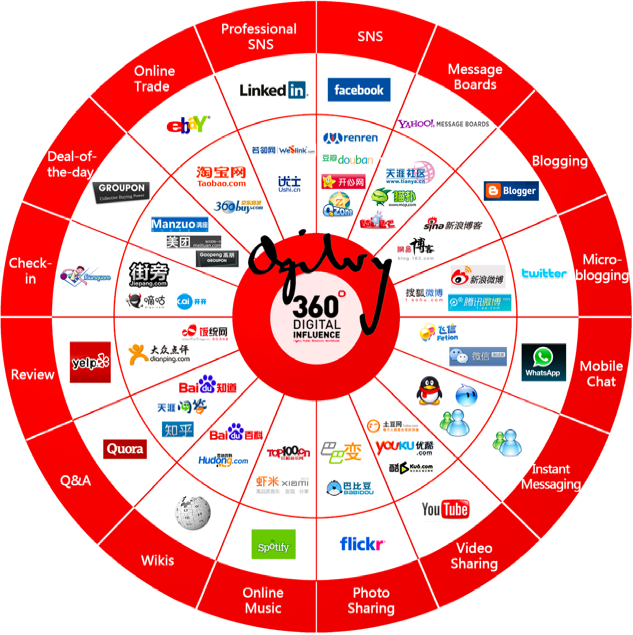
\includegraphics[height=340pt]{1-1.png}
%\caption{国内外社交媒体}
%\label{fig1-1}
%\end{figure}

社交媒体中的互联网用户不再是单纯的信息接收者,同时也是网络内容的产生者,人们通过社交媒体进行交流而获取和产生信息。以中国为例,目前拥有12亿手机用户、5亿微博用户、5亿微信用户,每天信息发送量超过200亿条,交流无处不在,无时不有。表~\ref{tab1-1}是互联网网站信息统计公司Alexa\footnote{网站地址:\url{www.alexa.com},访问时间:2014年9月。}统计的网络访问统计,从表中可以看出,根据统计,流量前十的互联网网站中社交媒体占了绝大部分。

\begin{table}[htp]
\centering
\caption{Alexa统计访问量前十名网站}
\label{tab1-1}
\begin{threeparttable}
 \begin{tabular}{|l|l|l|l|}
 \hline
 排名&网站&排名&网站\\
 \hline
 1& Google.com& 6&\textbf{ Wikipedia.org\tnote{1}}\\
 2& \textbf{Facebook.com}& 7& \textbf{Amazon.com}\\
 3& \textbf{Youtube.com}& 8& \textbf{Twitter.com}\\
 4& Yahoo.com& 9& \textbf{Qq.com}\\
 5& Baidu.com& 10& \textbf{Taobao.com}\\
 \hline
\end{tabular}
\begin{tablenotes}
  \centering
  \footnotesize
\item[1]表中加黑部分为社交媒体
\end{tablenotes}
\end{threeparttable}
\end{table}

那么究竟什么是社交媒体呢?社交媒体的典型代表维基百科是这样定义的\footnote{\url{http://en.wikipedia.org/wiki/Social media/}}:

\begin{definition}[Social Media]
Social media are media for social interaction, using highly accessible and scalable communication techniques. It is the use of web-based and mobile technologies to turn communication into interactive dialogue.
\end{definition}
从定义中我们可以看出,社交媒体是以互联网的思想和技术为基础的一项应用,用户可以借此进行内容创作、情感交流与信息分享。一般来讲,社交媒体可以分为如表~\ref{tab1-2}所示的几种类型。

\begin{table}[htp]
\centering
\caption{社交媒体的类型}
\label{tab1-2}
 \begin{tabular}{|l|l|}
 \hline
 类型& 代表性网站\\
 \hline
 维基(Wiki) & Wikipedia,Scholarpedia,百度百科\\
 \hline
 博客(Blogging) & Blogger,LiveJournal,WordPress,博客\\
 \hline
 新闻(Social News) & Digg, Mixx,Slashdot\\
 \hline
 微博(Micro Blogging) & Twitter,Google Buzz,新浪微博\\
 \hline
 评论(Opinion \& Reviews) & ePinions,Yelp,豆瓣\\
 \hline
 问答(Question Answering) & Yahoo! Answers,百度知道\\
 \hline
 媒体分享(Media Sharing) & Flickr,Youtube,优酷\\
 \hline
 书签(Social Bookmarking) & Delicious,CiteULike\\
 \hline
 社交网络(Social Networking) & Facebook,LinkedIn,MySpace,人人网\\
 \hline
\end{tabular}
\end{table}

从表中可以看出,社交媒体有多中不同类型,因此会产生多种不同形式的信息,包括文本、图像以及视频等。社交媒体上的信息由广大的社交媒体使用者产生,因此称为用户产生内容(User-Generated Content,UGC),这些信息依靠用户之间的关系与交互形成相互关联的庞大数据库。Kaplan和Haenlein\upcite{Kaplan2010}从数据和信息流动角度定义了社交媒体:首先是作为媒体(media),社交媒体中最突出的特点是它区别于电视、广播和报纸等传统媒体(信息的流动是从少数内容生产者到广大的信息消费者),内容产生的权利扩展到了所有的用户,而且信息流动的方式变得不确定,用户可以在内容消费者和生产者之间多次瞬间改变自己的角色;其次,作为社交工具,我们称这种新媒体是社会化的(social)的媒体,社会化意味着信息内容不只是由个体用户产生,更多是与其他用户的协作产生,信息的内容变得更加多样化,因此社交媒体不只是用来产生信息,也成为用户间互相交流通信以及传播信息的便利工具。

虽然社交媒体的出现为我们信息交流提供了便利,但是随着用户数量不断增加,产生的内容达到新的量级,导致我们作为信息消费者遇到了一些新的挑战,使得我们从“信息海洋”中找到有用信息变得更加困难,这通常称为信息超载(information overload)\footnote{信息超载描述了一种状态,就是当一个人在做选择时因为太多的信息而造成决策的困难。}。同时,由于社交媒体发布消息相对廉价和方便,内容产生门槛降低,任何人都能够参与其中,因此社交媒体中的数据出现了不同于传统媒体数据的新特点。
一般来讲,社交媒体中的数据具有以下特点\upcite{eisenstein2013bad}:
\begin{itemize}
\item \textbf{数量巨大(Big):}社交媒体中每个用户产生的数据可能不大,但是因为用户群体数量庞大,整体数据规模不可小觑,比如平均每天有超过300万条的微博(tweets)发布到Twitter\footnote{\url{http://www.twitter.com/}},每分钟有超过3000张照片上传到Flickr\footnote{\url{http://www.flickr.com/}},每年有超过160多万的博客(blogs)发表。
\item \textbf{广泛链接(Linked):}社交媒体的社会化特性使得用户产生的数据天生就是广泛链接的,最直观的就是用户产生内容往往由于用户之间的各种社交关系链接在一起,是一种新形式的大数据。这种链接的数据显然不是独立同分布的(IID,independent and identically distributed),对于想要使用传统的数据挖掘和机器学习方法研究社交媒体的研究人员是一种挑战\upcite{jensen2002linkage,taskar2003label}。
\item \textbf{充满噪声(Noisy):}社交媒体数据产生门槛的降低以及接入手段的增加,使得社交媒体的数据质量参差不齐,充满噪声\upcite{Agichtein2008}。不仅于此,社交媒体中的网络结构也充满噪声,一是网络中存在一些传播虚假和垃圾信息的用户\upcite{stringhini2010detecting},二是用户间建立关系的便捷性使得用户很容易将各种社会关系混杂在一起,无法区分好朋友和陌生人\upcite{xiang2010modeling}。
\item \textbf{非结构化(Unstructured):}社交媒体中用户产生数据,主要是文本数据,是高度非结构化的,尤其是随着移动互联方式的普及,越来越多的用户使用移动设备更新Facebook的状态,发送微博,或者回复别人的帖子,这不但导致了文本内容短小,而且错误拼写频繁出现\upcite{rossion1999spatio},经常还有一些非自然语言的使用,比如表情符(:),:()和缩写(h r u?)等\upcite{speriosu2011twitter}。
\item \textbf{不完整性(Incomplete):}为了保护用户的隐私,社交媒体平台一般允许用户将一些个人数据进行隐藏不被他人看到,这些数据包括个人信息,状态更新,朋友列表,发布的视频和照片以及与他人的信息交流等。比如Facebook仅有很少部分用户(小于1\%)公开了他们的个人数据\upcite{mislove2010you}。因此社交媒体的数据是极度不完整和稀疏的。
\end{itemize}

社交媒体的迅速普及与壮大,使得它在政治、经济、教育、社会等多方面发挥着越来越重要的作用。一些互联网公司开始以社交媒体大数据资源为支撑,以SaaS形式为用户提供服务。典型的如谷歌和Facebook的自助式广告下单服务系统、Twitter基于实时搜索数据的产品满意度分析以及国内百度推出的大数据营销服务 “司南”等。同时,政府也是社交媒体数据的积极使用者,2013年曝光的棱镜门事件显示出美国国家安全部门在使用社交媒体数据应用的强大实力,其应用范围之广、水平之高、规模之大都远远超过人们的想象。白宫2014年5月发布的《大数据:抓住机遇,守护价值》报告中重点提及了社交媒体大数据\footnote{来源:\url{http://www.whitehouse.gov/sites/default/files/docs/big\_data\_privacy\_report\_may\_1\_2014.pdf}}。
社交媒体大行其道的今天,自然也会成为品牌营销的手段之一,比如今年世界杯的主要赞助商之一可口可乐就首次挑选了粉丝在Facebook\footnote{\url{http://www.facebook.com/}}和Twitter上分享的照片,尝试进行iBeacon在社交媒体营销中的运用。
目前常见的社交媒体的大数据应用有:
一是基于用户个人信息、行为、位置、微博等数据而进行的个性化推荐、交叉推荐、品牌监测等营销类大数据应用,被互联网广告、电子商务、微博、视频、相亲等公司普遍采用。
第二,公共服务类大数据应用,即不以盈利为目的、侧重于为社会公众提供服务的大数据应用。典型案例如谷歌开发的流感、登革热等流行病预测应用能够比官方机构提前一周发现疫情爆发状况。国内也有搜索引擎公司提供诸如春运客流分析、失踪儿童搜寻的公益大数据服务。
三是积极借助外部数据,主要是互联网数据,来实现相关应用。例如,金融机构通过收集互联网用户的微博数据、社交数据、历史交易数据来评估用户的信用等级;证券分析机构通过整合新闻、股票论坛、公司公告、行业研究报告、交易数据、行情数据、报单数据等,试图分析和挖掘各种事件和因素对股市和股票价格走向的影响;监管机构将社交数据、网络新闻数据、网页数据等与监管机构的数据库对接,通过比对结果进行风险提示,提醒监管机构及时采取行动;零售企业通过互联网用户数据分析商品销售趋势、用户偏好等等。

随着社交媒体的迅速发展与参与用户的数目不断增多,社交媒体中可使用的信息也越来越丰富,具有广泛的应用前景。但是社交媒体中信息的庞大规模使得手工分析其内容变得十分困难,因此本文从信息自动化处理的角度对社交媒体的信息,主要是文本信息进行挖掘与分析,发现有用的信息,为社交媒体的相关应用提供帮助,本文特别关注社交媒体中的观点信息。
当然社交媒体与传统媒体存在显著的差异,其自身有不同的特点,我们将研究分析其特点为解决观点信息挖掘分析问题找到解决方案。


\subsection{观点分析}
%实际上文本信息有两种:事实信息与观点信息,事实信息是对事物的客观陈述。观点信息通常包含在博客、评论、回复或微博中,一般是由客户、读者或者公众用于表达表达自己的态度(attitudes),评价(appraisals),观点(perspective),情绪(sentiment)和情感(emotions)。用户不仅对产品(product)或服务(service)表达观点,也会对社会生活中各种话题(topic)或议题(issuses)表达自己的观点。
%观点挖掘或情感分析是自然语言处理(natural language processing)、机器学习(machine learning)以及文本挖掘(text mining)跨学科领域的研究,用于分析文本中对于产品、服务、话题或议题发表的观点,也称为情感分析或主观性分析(subjectivity analysis)\upcite{Liu2005}
%观点(opinion)一词起源于”opine“,通常”sentiment, view, feeling, belief, conviction, persuasion, notion, idea, and impression“为其同义词,词典中”opinion“被定义为信念,判断,个人的观点,态度,评价,思想,感觉和情感(belief , judgment , personal view, attitude, appraisal, thought , feeling, and emotion.)。观点的主要特点就是它是私人的感受,不是建立在证据和确定性基础上的。观点最终要有两个部分:目标(target)和情感(sentiment)\upcite{Liu2012}.
%实际生活中,别人的观点在决策过程中有时候是必不可少的信息。比如在商业领域,消费者在选择产品的时候常常需要知道其他人的对这些产品的评价,而商家为了市场营销也需要知道消费者的观点。在政治领域,投票者受到其他人关于候选人看法的影响而决定选择,同时大众的观点也会影响到政策制定者的政策决心。


信息分为两种,即客观信息和主观信息。语言学家Lyons\upcite{Lyons1977}将语言功能分为描述(descriptive), 社交(social)的和表达( expressive)三种功能。其中描述功能主要表达客观事实信息(factual information),而社交和表达功能往往表达的是个人的主观信息(subjective information)。主观信息,在语言中主要表现为观点信息,是人们在语言中表达对于谈论的目标事物的态度、情感或者看法\upcite{Wiebe2004}。观点常常简化为人对目标的同意或不同意(或者认为目标好或者坏,或持积极(positive)态度还是消极(negative)态度)\upcite{Rachels1986}等简单表示形式。总结起来,用户在社交媒体中表达的观点信息有三种类型:在评论、论坛、博客以及微博中针对某主题发表的个人体验(experience)和想法(opinion);关于新闻文章(artitle)、议题(isssues)、话题(topics)发表的评论(comments);在社交网站,比如Facebook上发表的个人状态更新(status)。

以往为了获取用户观点,需要进行问卷调查,而社交媒体的出现,为用户提供了全新的内容共享平台,使大量连接到网络的用户能够在各种社交媒体发表和表达自己观点:比如消费者可以在Amazon\footnote{\url{www.amazon.com}}, Yelp\footnote{\url{www.yelp.com}}, 以及TripAdvisor\footnote{\url{www.tripadvisor.com}}上发表各种商品和服务的评论;用户可以在Twitter\footnote{\url{www.twitter.com}}和Facebook\footnote{\url{www.facebook.com}}上对最新话题表达自己的观点。社交媒体上巨大的用户群以及由他们产生的海量信息成为了分析用户对各种话题所持观点的宝贵资源。
这些观点信息无论是对个人还是机构都起到非常重要作用。比如Horrigan\upcite{Hoffman2008}发现网络中发表的宣传信息对于网络用户在某些话题上观点的形成具有深远影响,用户表达的观点同样也是产品商家\upcite{Horrigan2008}以及政策制定者\upcite{Mullen2006}不得不考虑的重要因素,有证据显示这种观点的相互作用过程具有显著经济效果\upcite{Antweiler2004,Archak2007,Chevalier2006}。此外,大规模的用户看法整合形成的观点可以反映政治倾向\upcite{Tumasjan2010},甚至可以提高股票市场的预测\upcite{bollen2011twitter}。

社交媒体用户产生内容的大容量不可能依靠人工地去发现和总结其中的观点信息,因此需要计算机能够自动对观点信息进行分析和挖掘。观点分析\footnote{本观点分析包括了情感分析(sentiment analysis),观点挖掘(opinion mining)以及主观性分析(subjectivity analysis)等任务,都是对文本中的观点信息进行分析。}(opnion analysis)\upcite{Pang2008OMS}就是对文本中带有情感色彩的主观性信息进行分析、处理、归纳和推理的过程,其目的是自动发现和区分针对目标的情感和观点,目标可以是命名实体、也可以是话题或事件。
尽管语言学和自然语言处理已经有很长的研究历史,但是直到2000年才开始进行观点挖掘和情感分析等观点分析研究,从此观点分析成为了非常活跃的研究领域。特别是由于社交媒体的出现,研究者第一次拥有了大量的具有主观性信息的数据,正是有了这些数据,规模性的观点分析研究成为可能,可以说观点分析与社会媒体是一起起步和成长的,是社交媒体中数据分析的核心研究。观点分析研究不仅对自然语言理解(Natural Language Understanding)有着重要的影响,而且还对管理学,政治学,经济学和社会科学产生深远影响,因为它们都受到人的主观性的影响。

%
%
%观点分析(或观点挖掘)研究逐渐发展成为介于自然语言处理(Natural Language Processing)与自然语言理解(Natural language understanding)之间的一个独立领域,不像其他的自然语言处理任务(文摘或文本分类),观点挖掘主要处理与自然语言概念相关的语义信息和情感信息的推理而不需要对文本进行深度语法分析\upcite{cambria2014jumping}。

%如此巨大的信息量,主要是非结构化的(因为它是专为人类阅读消费产生的),因此不能直接使用机器处理的。文本的自动分析需要由机器对自然语言进行深入理解成,实际上我们距离这个目标还很远\upcite{6710245}。到目前为止,网上信息检索,汇总和处理都依据主要是依靠文本的文字表示方式。这些算法非常擅长于对文本进行检索,将其拆分,检查拼写和计算词语。但是,当涉及到解释的句子,提取有用的信息,他们的能力是非常有限的。这些基于词表示的算法的很大局限就是他们只能处理字面上的信息,而对于人类来讲,我们就不会收到这样的限制,因为我们看到的每一个字激活的语义相关概念,相关的情节和感官体验的级联,所有这些都使得我们可以以快速高效方式完成一些复杂任务(如词义消歧,文字蕴涵和语义角色标注)。计算模型试图通过模仿人类大脑处理自然语言的方式来弥补这样的认知差距,比如利用在未明确表示的文本语义特征。这些计算模型是有用既为科学目的(如探索语言交流的性质),以及用于实际用途(如能够有效地进行人机交流)。计算模型可以提供关于可再由心里语言学家(psycholinguist)进行探索的人类行为非常具体的预测。通过继续在这个过程中,我们可能最终会获得人类怎样进行语言处理深刻的理解。为了实现这样的梦想,需要具有前瞻性的思维心理语言学家,神经科学家,人类学家,哲学家,和计算机科学家的共同努力。
首先针对观点分析研究应该明确以下几个概念:
\begin{definition}[文档(Document)]
文档指的是自然语言中的文本片段,一般文档中至少会讨论一个话题。
\end{definition}
\begin{definition}[话题(Topic)]
本文中的话题可以是命名实体,事件,或者文档中提及的抽象概念(政治、健康、体育等)。
\end{definition}
\begin{definition}[情感(Sentiment)]
情感指的是文档作者针对话题表达的态度(attitude)、观点(opinion)或情绪(emotion)。
\end{definition}
\begin{definition}[情感极性(Polarity)]
情感极性值指的评价观点积极(positive)或消极(negative)程度的度量值,可以是一维的(打分值),二维的(积极值和消极值),也可以是多维的(喜怒哀乐等情感对应值)。
\end{definition}

针对观点有不同的定义方法,Liu\upcite{Liu2012}将观点形式化定义为观点五元组$ (e_i,a_ij,s_ijkl,h_k,t_l)$,
其中,$ e_i $是目标名称,$ a_{ij} $是目标的不同属性(方面,aspect),$ h_k$是持有观点的用户,$ t_l$表示时间,$ s_{jkl}$是观点的情感值。
Kim和Hovy也对观点做了定义\upcite{Kim2004},认为观点由四个元素组成:即主题(Topic)、持有者(Ho1der)、陈述(Claim)、情感(Sentiment)。
他们认为观点分析就是发现和确定各个元素的过程。
总体来看,比较全面的观点分析可以认为是由三个主要步骤组成:
\begin{itemize}
\item \textbf{文本中观点信息确定:}需要确定文档中涉及的话题信息,将不同话题对应的文本片段进行对应联系起来,并且需要对文本片段进行主客观分离找到主观性文本,因为观点一般是从主观性的文本中确定的。将主客观文本分离一般需要一些明显带有情感的词语作为标志,这些词语集合在一起形成了能对情感知识进行表示的情感词典。
\item \textbf{文本情感分类:}从文本中抽取有用的特征将文本分为不同的情感类别,一般是将文本分为积极或消极极性(或者中性,即客观文本),主要使用机器学习的各种方法,或者基于规则的方法。
\item \textbf{观点的集成表示:}经过前面两步,得到了主观文本片段以及文本片段中的具体观点,观点的集成是在更高的层次上的观点分析,是将文本片段中分散的观点整合集成成为一个观点,并根据不同的应用需求以一种合理的方式表示,比如可以见同一作者的所有文本片段中的观点集成起来,称为用户的主观性模型,或者将文本片段按照时间前后串联起来形成观点随时间的演化表示。
\end{itemize}

观点分析有别于传统的话题分析。话题分析关心的是文本所阐述的客观话题,如文档是属于教育类还是娱乐类的,而观点分析主要用来识别文档中表达的观点、喜好、立场和态度等主观信息,需要分析文档的词语语义、词性,甚至句法和篇章结构等信息。在传统的话题分析中,主题词是最重要的特征,而在观点分析中,情感词是最重要的特征。观点分析涉及语言学领域的诸多问题,由于语言的复杂性和多样性,需要面临以下几个问题:

\begin{enumerate}
\item \textbf{领域相关性:}某些情感词在不同的领域中具有不同的情感极性,比如 :``轻薄 '' 在通常意义下具有消极极性,如 ``举止轻薄'',而在电脑领域,``轻薄 ''却表示褒义,具有积极极性。
\item \textbf{语境依赖性:}某些词语具有多个词性,并且不同的词性常常呈现出不同的情感极性。比如``这款空调经济耐用''和 ``经济呈现快速发展'' 在这两句话中,``经济'' 具有不同的词性和情感极性,前者是形容词,具有积极情感极性,后者是名词,具有中性情感极性。
\item \textbf{上下文相关性:}语言中有许多词语本身是不具有情感极性的,但是在特定的上下文环境中,语言描述便具有了情感极性。比如:``小''、``高''、``快'' 等词语,在搭配组合``损失小''、``成绩高''、``进歩快''中,具有积极情感极性,但在搭配组合 ``心眼小''、 ``耗油高''、``耗电快'' 中,则具有消极情感极性。
\end{enumerate}

%情感词典,是人们在表达观点时常用的一些词语,是主观性信息的最明显的证据(比如``好'')。无论对无监督还是监督方法,因此一部好的情感词典是从文本信息中发现主观信息的重要特征。近年来从网络数据中发现主观性信息变得越来越重要,能够获得大家对一些事物、人或事件的主观性态度比仅仅只有百科式描述更重要,比如对产品的问卷调查,政治选举的民调以及商业广告效果分析等。因此很多研究者开始注意到这种信息需求,并试图从网络数据中挖掘并分析主观性信息。然而大多数工作主要关注与于本中情感倾向的总体以及详细的分析,并且仅仅是对某些特定领域的文本数据,比如产品评论或博客,并不适用于其他类型数据。随着社交媒体的普及,用户可以更方便地发表与自己有关的信息,比如自己的生活和对周围食物的观点,这些越来越多的用户产生数据使得主观性信息的挖掘和分析变得更重要。受到这种趋势和研究需求的影响,TREC评测\footnote{\url{http://www.trec.state.tx.us/}}从2006年开始就有关于从网络信息中挖掘观点的评测,并且受到很多自然语言处理研究人员的关注。判断一片文档是否有主观性信息最简单直观的方式就是看看是否含有主观性词语,这种基于词语的判断方式的基本假设就是文档中含有主观性词语通常是表达作者的主观观点,比如在商品评论中出现``喜欢''通常表示作者喜欢这个商品。因此很多研究者研究了一些通过人工或自动方式产生带有主观情感倾向的词典。
%
%主要有两种类型的网络上的信息(即,事实和观点)。然而,目前的搜索引擎(如谷歌),都是为了表达同主题关键字的事实。Wiebie\upcite{Wiebe1994}将带有个人心理视角的文本称为主观性信息,相对于客观地叙述事件或描述虚构世界的文本。Dave等\upcite{Dave2003}提出了观点挖掘作为从网络数据中发现主观性信息的研究。观点是所有人类活动的中心因为观点是我们行为的关键影响因素,我们对现实世界的感知和看法是建立在他人是怎么看这个世界的基础上的,当我们做决策之前通常会寻求其他人的观点。随着社交媒体的出现并流行(评论,论坛,博客,微博,评论,以及在社交网络中的帖子等),带有主观性信息的数据爆炸式增长,因此我们对观点信息的获取不再需要靠传统的问卷调查等手段。然而发现并综合各种社交媒体中观点信息并不是意见容易的事,因为数据量非常大之外,人工阅读并发现主观性信息是不可能的,因此需要自动观点挖掘技术。近年来,在社会化媒体带有主观性信息的贴子在我们的现实生活中帮助重塑了企业,并左右公众的情绪和情感,这对我们的社会和政治制度深刻影响。这样的帖子对于鼓动群体运动引起政局变化具有很大作用,比如2011年发生在一些阿拉伯国家的阿拉伯之春运动。因此收集和研究在网络上的意见成为一种必然。情感分析应用已经普及到几乎所有可能的领域,从消费产品,服务,医疗保健和金融服务等社会活动和政治选举。除了现实生活中的应用,很多应用为导向的研究论文也已发表。例如,情感信息可以预测产品的销售量\upcite{Liu2007},电影的票房\upcite{Oghina2012,Joshi2010,Sadikov2009,Asur2010},股市走向\upcite{Zhang2011,bollen2011twitter},政治选举的结果\upcite{Tumasjan2010,Chen2012,Metaxas2011,Gayo-Avello2011,Armstrong2011}等等。
%
%由于具有许多挑战性的研究问题和广泛的实际应用价值,观点挖掘和情感分析在过去的十年一直是非常活跃的研究领域。所有情感分析研究围绕一系列的任务,包括极性分类\upcite{Pang2004},观点抽取\upcite{Ding2009}以及观点源设定\upcite{Zhao2010}。
%
%大多数方法严重依赖于标注语料训练情感分类器,因此情感标注语料可以说对情感分析是非常珍贵的资源。本章最重要的一个目标就是减轻费力的标注过程,发展一种无监督的情感分析方法。
%
%在文本情感分析中,中文与英文的分析方法有所不同,中文首先要解决文本切词的问题,其次在特征提取方 法和情感词典构建等方面都存在一定差异。目前国内针对中文情感分类的研究相对较少,有采用类似英文情感分类方法的研究,朱嫣岚等人利用知网计算待定词与基准词间的相似度来判断其倾向性\upcite{朱嫣岚2006}。
%然而过去的情感分析研究主要是针对英文社交媒体(比如review以及Twitter),很少有工作致力于中文社交媒体的研究,就我们所知,在对中文微博的研究中,主要是开始进行一些基本的介绍和预测\upcite{Guo2011,Yu2011},近些年开始进行特点分析\upcite{Tian2012}以及用户微博行为分析\upcite{Gao2012,zhang2008review}。本文中,我们特别关注于中文的情感分析尤其是微博和产品的评论,进行了一下方面的研究(1)通过分析中英文情感词典的不同特点,根据情感知识相通的前提,使用语义知识词典根据对应语义关系将英文情感词典的情感知识转移到中文词语形成新的中文情感词典,减少了人工区分和标注;(2)研究英文情感词语的扩展方法在中文环境下的性能,并根据中文特点提出相应的语法特征以及统计特征,通过混合方式在中文社交媒体语料中扩展和构建情感词典;(3)基于使用机器学习方法进行情感分类框架,依据中文中情感表达的特色,对情感分类特征空间进行改进,更新分类模型,提出了一种无监督的中文微博情感分类方法。
%
%与事实信息为基础的分本分类相比,观点信息的分类通常类别会少一些,可能只包含正面负面情感极性(sentiment polarity)或者序号类别(ordinal categories),因此观点信息的抽取一般是关注于观点表达方式抽取(比如情感类型以及强度),比事实信息抽取(话题、事件、实体等)相对来讲看起来好像简单,实际上并非如此。事实信息因为与话题相关的关键词的不同而在不同话题的文本中差别很大,因而容易区分,可观点信息并非如此,因为情感的表达是以一种细致的方式表达,因而单靠只言片语很难确定,需要以来与具体的上下文语境,同一个表达方式在不同领域可能表达了不同的情感类型。这些都是观点信息分析的挑战和吸引之处。
%
%总体来讲,情感分类研究可以分为基于词典和基于学习的。简单来说,基于词典的方法是使用人工或者自动编辑的词表(比如“喜欢”等),并认为这些词语的出现是观点的标志;而对于学习方法来说,主要是依靠词语共现来使用已有分类的数据实例来训练产生分类器进行自动分类。

\section{研究问题}
\label{point}
随着以Twitter,Facebook、新浪微博为代表的社交媒体迅速发展,人们越来越愿意在线分享自己的看法、观点以及体验,他们可以选择博客写作、微博发帖、社交网络状态更新、发表产品评论、或者在论坛中参与讨论发表对于任何话题的看法和观点,因此网络被各种各种意见所充斥,现在的网络可以说是一个“观点网络”,网络已经成为获取观点信息的主要来源。但是站在网络使用者的角度,一方面可以很容易获得大量的带有观点的信息,这些信息远远超出了个人的处理能力,因此用户面临着“信息超载(information overload)”问题;另外一方面,观点的主体是人,而网络中的信息尤其是社交媒体中的信息多是以“碎片化”的形式存在,个人观点分散在许许多多多的信息碎片中,使得用户真正的信息需求(能针对目标主题及时准确从网络中找到公众或个人观点)变得更加困难,因此用户又面临“信息不足(information shortage)”问题。传统的信息检索技术,尤其是搜索引擎,很难解决这样矛盾的信息供求关系。当然目前已经有观点检索系统\upcite{he2008effective,macdonald2007overview,ounis2011overview},可以解决如“检索评价某产品的文档,并总结其中的观点”这样的问题,但是还不能满足“大家对某产品的观点或某个朋友对该产品的观点”这样的信息需求。因为这样的问题需要就网络中,尤其是社交媒体中每个用户的观点进行挖掘、分析并整合集成。网络中的信息,一个事实信息可以代表所有的事实信息(One fact stands for all facts),但是一个观点不能代表所有的观点(one opinion can not represent all opinions)。
从用户的角度来说,一条信息中的观点可能只是他就话题的某个方面表达出的观点,就话题整体的观点需要将所有分散在“信息碎片”中的观点进行集成,并以一种合理的形式表示出来,才能代表一个用户真正的观点。
因此本文首先从下面一个科学问题出发,来研究观点分析:

\textbf{怎么样才能准确的对社交媒体中用户的观点进行表示和分析?}

这个问题需要从挖掘用户的信息碎片中的观点出发,是一个观点信息确定、分类以及整合的过程,需要解决文本情感知识表示,情感倾向性的分类以及观点信息的集成等问题。

反过来,因为人是具有主观能动性的,人的行为会受到自己观点和思想的影响。用户在使用社交媒体时会有多种交互行为,比如信息传播行为,人们通过转发分享新闻与观点,加速信息的流动、扩大信息传播的范围。用户的信息传播行为同样会受到自己的主观性的影响,通过观点的分析与与集成可以对用户的主观性进行建模,而用户的主观性模型无疑会对分析用户的一些在线的信息交互行为有帮助。因此本文从以下两个科学问题出发来研究用户的主观性建模,并分析其对用户传播行为的影响:

\textbf{用户的主观性如何表示和建模?}

\textbf{怎么样使用主观模型分析用户的信息传播行为?}

用户在社交媒体中的产生的内容会涉及到多种话题,而且会对话题的不同方面发表观点,因此回答第一个问题需要研究用户产生信息中多样性话题的确定及表示问题,还有用户在不同话题上多种观点的集成及表示问题。
在信息传播过程中,用户作为带有自己主观判断的传播主体,会在不同情况下产生传播行为,因此回答第二个问题需要首先确定用户传播行为产生的具体原因,然后研究怎么样从主观动机角度对这些原因度量分析。

\section{相关研究}
本节主要介绍与观点分析与用户传播行为分析相关的一些现有工作,其中观点分析包括观点挖掘,观点集成两个部分相关工作。
本文的相关工作分析主要从整体相关工作和局部相关工作进行阐述,本章的相关研究主要介绍的是整体的相关工作,因为这些研究成果可以为本文所研究的具体任务提供思想借鉴和技术支持。以后各个章节中的相关工作则会具体地分析已有的类似工作,以及研究成果。
特别需要强调的是,无论是观点分析还是传播行为分析,对社交媒体中文本的处理都是其中一个重要的环节。社交媒体数据的一些特性已经在第~\ref{ch1_social}节有所介绍,这些特性造成自然语言处理技术在社交媒体上的应用存在着新的挑战,使用自然语言处理技术对社交媒体文本进行处理,主要工作包括文本规范化(Normalization)\upcite{eisenstein2013bad,toutanova2003feature,gimpel2010part,owoputi2013improved},领域适应化(Domain adaptation)\upcite{finkel2005incorporating,ritter2011named,foster2011news,
han2011lexical,han2012automatically,han2013lexical,liu2012joint,liu2012broad,Hassan2013,gimpel2010part,owoputi2013improved,finin2010annotating,
ritter2011named,liu2011recognizing},预处理(preprocessing)\upcite{li2012twiner,liu2012joint,liu2013named}以及进行一些结构化处理(词性、句法、标注等)\upcite{liu2012two,sharifi2010summarizing,chakrabarti2011event,
takamura2011summarizing,weng2011imass,harabagiu2011relevance,Ren:2013:PTT:2484028.2484052,shen2013participant,judd2013better,chang2013towards,
finin2010annotating,ritter2011named}。

\subsection{观点挖掘}
\label{ch_mining}
观点挖掘研究识别文档中针对一主题表达出的观点以及这观点的极性(例如,是积极还是消极)。观点挖掘通过对文档深入分析得到文档中表达的观点信息,是观点分析后续任务的基础,观点挖掘的结果影响着后续分析任务。一般观点挖掘包含观点识别(identify)和极性分类(classify)两个步骤。观点识别主要是从文档中识别出话题以及与话题相关的带有观点的文本片段。识别带有观点的文本片段(一般是文档中的句子)也称为主客观分析(subjectivity analysis),是将文档中的带有观点的句子与描述客观事实的句子区分开,研究表明将文档中的客观文本过滤有助于提高观点挖掘的准确性\upcite{Schler2005},目前主客观分析主要采用机器学习方法进行主客观分类\upcite{Wiebe2001,Wiebe2005,Dave2003,Pang2004,Riloff2005,Wilson2009}。极性分类是将文档就话题表达出的情感倾向进行极性分类,一般是分为积极与消极,也可以是多种类别(当类别为积极、消极以及中性时,与主客观分类一致)。
观点挖掘研究方法一般可以分为基于词典、基于统计以及机器学习三类。

\subsubsection{基于词典的观点挖掘}
基于词典的观点挖掘依赖于预先构建好的情感词典,词典里的词语都标注了情感极性值。常用的英文情感词典有General Inquirer\footnote{\url{http://www.wjh.harvard.edu/~inquirer/}},DAL(Dictionary of Affect of Language)\footnote{\url{http://www.hdcus.com/}},WordNet-Affect\footnote{\url{http://wndomains.fbk.eu/wnaffect.html}}以及SentiWordNet\upcite{Baccianella2010}。
基于情感词典的方法一般是用词典确定文本中的带有观情感极性的词语,用以判断文本是否主观文本。也有一些研究使用情感词典词语的情感极性值来计算文本的观点极性\upcite{Angel,Tsytsarau2010,Missen2009},一个句子或文档的极性值可以通过将每个词语的极性值取平均来确定,常用的计算方法可以使用公式~\ref{eq1-5}来表示:
\begin{equation}
\label{eq1-5}
S(D)=\dfrac{\sum_{w \in D}S_w \ast weight(w) \ast modifier(w)}{\sum weight(w)}
\end{equation}
其中$ S_w $是文档中的词语在情感词典中的极性值,$ weight(w) $是权重函数,可以根据词语相对于话题词的位置进行权重调整,$ modifier(w) $是专门处理否定、增强或其他改变词语情感值的一些修饰操作。
典型工作如Zhu等\upcite{Zhu2009}首先将文档或句子中词语的极性值累积在一起,然后使用简单的基于规则算法计算整个文档或句子的极性值。一些比较成熟的情感分析工具,比如Sentiment Analyzer\upcite{Yi2003},或Linguistic Approach\upcite{Thet2009}针对话题挖掘一些领域相关特征、观点句的模式或词性标签等作为规则加入到文档极性值的计算中,可以得到更精确的极性值,但是需要增加计算复杂性。

\subsubsection{基于统计的观点挖掘}
这种方法是基于语料中表达相似观点的词语经常会出现在一起这一观察基础上的,因此,如果两个词语频繁在同一上下文中同时出现,它们就很有可能有相同的极性。因此一个词语的极性值可以根据它与一个极性恒定的词语(比如“good”)共现的频率来确定。Turney\upcite{Turney2002,Turney2003}提出使用点对点互信息(point-wise mutual information (PMI))\upcite{Church1990}作为统计依据来计算词语的共现:
\begin{equation}
PMI(x,y)=\log_2\dfrac{F(x,y)}{F(x)F(y)}
\end{equation}
其中$ F(x,y) $表示两个词语的共现频率,$ F(x) $表示词语的出现频率。词语$ x $的极性值可以通过计算该词语与两个相反极性词语的互信息差值来确定:
\begin{equation}
PMI-IR(x)=\sum_{p \in pWords}PMI(x,p)-\sum_{n \in nWords}PMI(x,n)
\end{equation}
其中$ pWords $表示积极极性的基准词集合,$ nWords $表示消极极性基准词集合。为了统计词语出现频率,Turney使用AltaVista搜索引擎检索词语返回的条目数作为词语出现频率。Chaovalit和Zhou\upcite{Chaovalit2005}扩展了Turney方法,通过谷歌搜索引擎确定词语共现频率,提高了准确性。Read和Carroll\upcite{Read2009}使用语义空间和分布相似性作为替代方法进一步扩展了Turney方法。这种方法更细致的全面的研究是Taboada等\upcite{Taboada2006},他们提出了使用搜索引擎确定共现频率的一些问题。Ben等\upcite{he2008effective}提出使用统计方法构建情感词典与信息检索相结合的方法获取主观性的博客文档。

\subsubsection{基于机器学习观点挖掘}
在观点挖掘研究早期,机器学习方法和标注数据集的使用加速了研究的进展,目前最常使用的仍然是机器学习方法。机器学习方法是对分类问题的比较成熟的解决方案,一般经过训练和预测两个过程,可以进行如下形式化表示:假设训练数据集是经过极性标注的文档集$D$,每个文档都可以用特征(词语,二元组等等)向量表示,文档都被标注了情感极性(在极性空间$S$中的一个值),机器学习的训练过程可以形式化为,给定训练数据集:$ \{(d,s)|d \in D,s \in S\} $,找到映射:
\begin{equation}
g:D \rightarrow S,\quad g(d)=\arg max_S f(d,s)
\end{equation}
极性分类也就是找到映射$ g $,将文档根据打分函数$ f $映射到情感极性空间,函数$ f $以文档向量和标注的极性作为输入,对未标注的文档给出极性预测的概率值(使用条件概率或联合概率),训练的过程就是对打分函数$ f $的估计过程。一般训练过程有以下几个步骤:
(1)首先获取训练数据集,数据集可以是带标注的(有监督),也可以是无标注的(无监督);
(2)在文档集中发现有用特征,将文档使用特征向量表示;
(3)通过分析相关特征共现规律,训练分类器区分文档极性标签;
(4)最后使用训练得到的分类器对新文档预测给出极性概率值。

Pang和Lee\upcite{Pang2002}最先将机器学习方法引入了观点挖掘领域,作者提出了使用三种有监督的分类器(Naive Bayes (NB),maximum entropy (ME)和support vector machines (SVM))进行电影评论的情感分类,三种分类器都能超过随机选择的基准分类器,平均准确率达到80\%,其中SVM表现出最好的性能。Dave等\upcite{Dave2003}扩展了Pang的工作,强调使用特征选择对情感表示特征进行过滤,可以将准确率提高到87\%。Pang和Lee使用主客观分析对文档进行预处理,过滤掉其中的描述客观信息的句子,发现可以提高极性分类的准确性。后续的一些工作主要集中于研究如何扩充有用的分类特征\upcite{Melville2009,Vegnaduzzo2004,Devitt2007,Osherenko2007},训练数据的构建\upcite{Goldberg2006,Taeckstroem2011}以及机器学习方法的选择\upcite{Mcdonald2007}。

\subsection{观点集成}
\label{ch_integrate}
通过观点分析得到的是单个文档中的观点信息,实际使用的时候,我们关注的是更高层次的观点,而不是单独一篇文档的观点,因此需要对文档观点分析结果进行整合集成。这种整合集成可以按照不同的维度进行,比如为了了解一群人的观点分布,需要将每个人发表的所有文档中的观点进行集成。最需要观点集成的研究领域是产品评论,需要从大量用户发表的评论中抽取出产品的特征,并计算不同用户针对相同特征的观点或打分的平均值,以便进行观点集成形成对产品总体的评价。以图~\ref{fig1-2}所示产品评论的观点集成为例,观点集成一般包括信息收集,观点识别,观点分类以及推理集成三个步骤\upcite{Tang2009,Liu2005,Ng2006}。
\begin{figure}[htp]
\centering
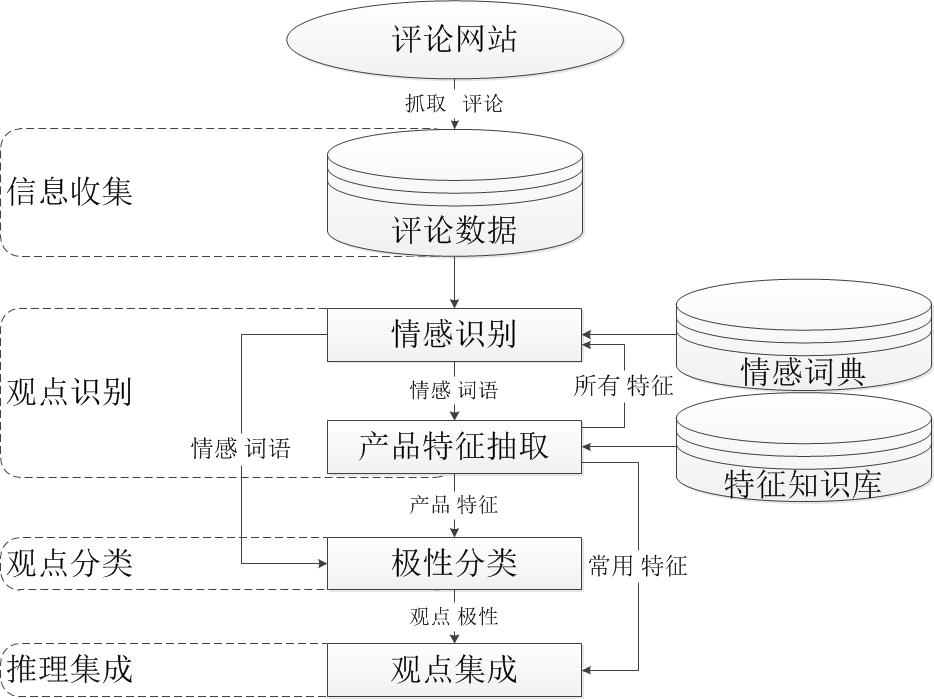
\includegraphics[height=220pt]{1-2.jpg}
\caption{产品评论的观点集成框架}
\label{fig1-2}
\end{figure}

对于文档集$ D $中的针对某话题的观点进行集成形式化表示为:
\begin{equation}
\{(f,s_f)|rep(f,D)>\rho_f,s_f=agg(S,f)\}
\end{equation}
其中$ f $表示根据某种表示度量方法$ rep(f,D) $确定的描述话题的不同方面,$ s_f $是针对$ f $根据集成函数$ agg(S,f) $计算出的针对$ f $的观点。

观点集成一个主要的挑战就是如何确定描述话题的多个不同方面。Leouski等\upcite{Leouski1996}评测了各种文本聚类方法对检索结果中信息的集成效果,发现聚类方法对于文本的交互式检索是有用的。Zeng等\upcite{Zeng2004}使用监督学习方法从文本中抽取主要短语并将其聚类表示话题的方面。越来越多的工作使用生成模型发现文档中的隐性方面话题\upcite{Su2006,Titov2008},还有一些工作使用数据挖掘中的联合规则方法对产品的相关方面进行挖掘\upcite{Liu2005,Popescu2007}。

\subsection{传播行为分析}
\label{rel3}
社交媒体中信息传播具有重要的应用价值,信息传播的主体是人,也就是社交网络的用户,研究人的传播行为是研究信息传播的重要组成部分。社交媒体中最具影响力的是微博上的信息传播,因为用户在微博的转发行为会使得信息在短时间内形成大规模的传播,因此本文主要从微博的转发行为来阐述相关工作。微博的典型代表是Twitter,Twitter转发机制,即重新发布其他人发布过的微博,以便于作者的全部粉丝看到转发的信息,使得信息迅速形成病毒式传播(viral propagation)。很多对于转发行为的研究分析涉及影响转发行为的因素,包括tweet的文本内容与转发的关系,用户的属性如何决定其他人的转发;Twitter中信息的一般传播路径与规律等等。

Boyd等人研究了Twitter中转发的各种类型以及转发的原因,他们分析了不同用户,用户属性,用户交流方式对于转发的影响,同时也分析了人们在Twitter中喜欢转发的内容\upcite{boyd2010tweet}。他们发现18\%的转发tweet包含hashtag,52\%的转发tweet包含链接,11\%的转发tweet包含连续的转发符号串(如,“RT @user1 RT @user2 ”),另外,9\%的转发tweet都包含回复原tweet作者的回复字符串(“@reply”)。这说明tweet文本中的hashtag,链接、回复、提交和转发符号都与tweet的转发存在着一定的对应关系。

Yang和Counts通过Twitter中的提及(“@username”)抽取了用户之间的关系,并在此基础上构造了用户关系的复杂网络。他们研究了信息在这个复杂网络上是如何传播的,包括信息传播的速度,规模,以及范围\upcite{yang2010understanding}。他们发现大约只有25\%的tweet是被信息作者的朋友转发,大部分是被粉丝但非朋友转发。这说明Twitter中用户形成的复杂网络,影响着人们的转发行为,因此信息在传播路径上具有一定的规律可循。

Macskassy和Michelson分析了一个月用户的Twitter数据,他们解释了各种信息传播的方式,尤其是转发的行为模式,他们发现tweet的内容是tweet被转发的决定因素,因此他们构建了基于内容的转发模型\upcite{Macskassy2011}。

Starbird等人对具体事件在Twitter上的传播进行了深入研究,他们分析了2011年埃及的政治事件,演示了这个事件的相关信息在Twitter上是如何生成,发展,传播的\upcite{starbird2012will}。

Comarela等人研究了影响用户回复或转发的因素,他们发现以前是否回复,发布信息的频率,信息的时效性,tweet的长度决定用户是否回复\upcite{comarela2012understanding}。

除了以上的工作,最新的研究还从不同角度对Twitter中的转发行为进行了深入的研究\upcite{kupavskii2013predicting,jenders2013analyzing,ahmed2013peek,bao2013popularity}。

综上所述,影响用户转发行为的因素主要包括tweet文本的内容、tweet文本的社交媒体属性(如是否包含链接、hashtag、提及等)、tweet作者的用户属性,tweet作者的朋友圈子,当然以上的研究都是从宏观上大规模分析Twitter转发数据得出的研究结论。从微观的角度则可以考虑给定一个tweet,未来这个tweet是否会被转发,是一个值得研究的问题。

虽然已有的Twitter转发研究从许多不同的角度进行了考虑,但是还没有工作从用户的主观动机角度进行研究,本文我们将结合用户观点分析研究的结果对转发行为进行分析。另外,目前的转发大多都是从tweet本身进行考虑,并未从受众的角度进行分析,本文将对tweet、作者、受众三个方面在转发过程中的相互关系进行探讨。

\section{研究内容与方法}

\subsection{本文研究内容}
本文的研究内容主要是围绕社交媒体上的观点信息的分析应用,从两个角度对用户产生的带有观点的内容进行建模:一个角度是从不规范的社交媒体文本中发现观点信息,并在用户层面进行观点集成对用户的主观性进行建模,另外一个角度是利用用户产生内容中分析得到的用户主观模型分析用户在使用社交媒体时的一些在线行为,本文主要分析用户在微博的转发行为。研究框架如图\ref{fig1-3}所示。

\begin{figure}[htp]
\centering
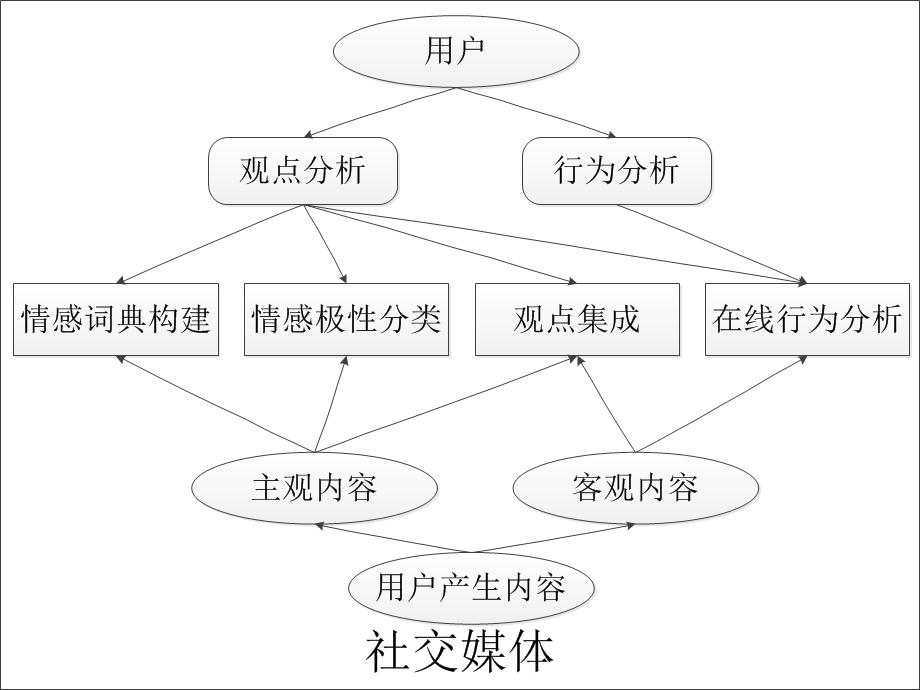
\includegraphics[height=230pt]{1-3.jpg}
\caption{本文研究框架}
\label{fig1-3}
\end{figure}

本文主要研究内容分为四个部分:首先从社交媒体文本中得到观点信息属于观点挖掘研究内容,观点挖掘方法分为基于情感词典和基于机器学习的方法,因此需要进行\textbf{情感词典的构建研究}以及判断观点极性的\textbf{情感分类研究};其次从社交媒体文本片段中挖掘到的观点需要进行整合集成,变成具有代表性的观点信息,属于观点集成的研究内容,我们将从用户维度对用户的所有观点进行集成,用于\textbf{用户主观性建模};最后利用用户的主观模型,从行为主观动机角度对用户的信息传播行为进行分析,属于\textbf{转发行为分析}研究内容。
具体四个研究内容的阐述如下:

\begin{enumerate}
\item \textbf{情感词典的构建}:使用已有的比较成熟的英文情感词典中的情感知识进行跨语言情感知识转移,构建一个通用的中文情感词典;针对通用情感词典领域适应性弱的问题,通过基于语料库情感词典扩展研究,使用语料中的语言特征以及统计特征,对情感词典在领域内进行扩展以增强情感词典的领域适应性。
\item \textbf{情感分类}:根据社交媒体情感表达方式的领域依赖性,对情感分类特征空间进行分割,将领域独立的通用特征与领域依赖特征分开,使用两部分特征分别训练分类器,通用分类器使用现成资源训练,领域分类器使用远监督方式训练,最后两个分类器在自举式机器学习框架下组合成性能更强的情感分类器。
\item \textbf{用户主观性建模}:提出一个通用的主观模型定义,将用户产生内容中关注的话题和针对这些话题表达的观点组合在一起,对用户在每个话题上发表的所有观点整合集成,并使用一个在情感极性值空间中的分布表示用户在话题上的综合观点,使用一个更简单通用的框架构建主观模型。
\item \textbf{转发行为分析}:构建好每个用户的主观模型后,给定微博,发现作者的粉丝中,谁会在未来传播微博,从用户的主观动机角度,分析用户在三种转发情形下的主观动机,即微博内容的吸引力,转发微博的社交需求以及转发微博的认同需求。
\end{enumerate}

总的来说,针对~\ref{point}的第一个问题,本文通过构建情感词典识别社交媒体中带有观点的文本信息,并使用无监督的情感分类方法对观点的极性进行分类;
针对~\ref{point}的第二个问题,本文通过将用户关注话题与发表的观点进行组合建模,采用集成的观点表示方式对用户的主观性进行建模;
针对~\ref{point}的第三个问题,本文通过计算主观模型之间的相似性度量用户一些在线行为的主观动机,进行行为的分析。

\subsection{本文研究方法}
社交媒体中的观点分析涉及到信息检索、机器学习、自然语言处理与自然语言理解等多方面的方法和技术,这些方法和技术的综合使用是由社交媒体数据特有的性质以及观点分析应用的特殊需求所决定的。
从社交媒体数据特性来看,进行观点分析需要面临以下挑战:
\begin{itemize}
\item 社交媒体中的文本篇幅较短而且噪声较多的特点,使得利用标准的机器学习方法进行分析面临数据稀疏问题,也造成自然语言处理技术的困难;
\item 庞大的数据容量以及动态的语言特性造成通用的标注数据的匮乏,无法满足机器学习训练要求;
\item 社交媒体是一个开放平台,文本涉各种领域,因此各种方法和技术都要满足多领域环境的需求;
\item 社交媒体中的数据以数据流的形式不断高速增长,需要能够快速适应新数据并实时处理的技术和方法。
\end{itemize}

观点分析需要从大量的社交媒体用户产生的内容中发现观点信息,进而进行整合集成并用于分析用户的转发行为,要解决以上问题和挑战,需要达到如下几个主要目标:
\begin{enumerate}
\item 使用文本规范化和消除噪音等自然语言处理技术对数据进行预处理,数据的稀疏性需要得到缓解,然后才能进入后面的分析中;
\item 观点极性分类方法应该具有领域独立能力,当领域变化时能够快速适应并且性能不能下降;
\item 采用的所有技术和方法能够以有限的计算能力分析和处理不断增长的数据;
\item 针对训练数据缺乏问题,尽量使用无监督或者弱监督的方法和技术,并且尽量使用已有的资源,减少人工标注。
\end{enumerate}  

针对以上挑战和目标,我们确定的研究方法为:

首先在数据和资源选择上,我们首要选择已有的知识资源和标注数据。如果没有对应的知识资源,可以通过资源转化变成我们想要的知识资源,比如情感词典构建时,我们通过情感知识之间的对应关系,将英文情感词典转化为中文情感词典。如果没有直接标注数据,我们选择采用弱标注的方法得到训练数据,所谓弱标注数据指的是,数据的类别标签是通过启发式从数据中直接确定不需要人工标注,比如在训练情感极性分类器时,我们使用含有明确情感极性的成语微博作为训练数据,是基于微博短小观点表达相对会集中在一些极性相同的词语身这一假设,从而获得大量训练数据。在理想的情况下,用弱标记数据的好处是双重的:首先,我们可以以接近零的代价采集训练数据,因此可以轻松地将我们的应用扩展到其他领域或语言。其次,弱标注语料的规模可以很容易超越常规手动标注的训练语料的数量级。

在学习训练方法的选择上,我们优先选择无监督或半监督的机器学习方法。无监督或办监督学习方法可以减少或无需大量的标注训练数据,而且可以通过迁移方法将学习到的知识进行跨领域或语言转换。比如我们在对微博进行极性分类时,使用自举式机器学习方法将两个弱的分类器结合在一起提高了分类的性能;在构建主观模型时,我们使用LDA话题模型识别用户关注的话题,并使用基于规则的情感分析方法获得用户的观点信息。  

\section{本文主要贡献}
本文以用户为单位,对用户在社交媒体上产生内容中的观点信息进行识别、分析和集成,并使用得到的观点信息分析用户在社交媒体上的在线交互行为,具体来说本文的主要贡献为:
\begin{itemize}
\item 设计了一种中文情感词典的自动构建方法,该方法能够从已有的英文情感词典通过词语之间的对应语义关系转化情感知识,并且能够针对任何领域的语料进行扩充,成为准确性更高的领域情感词典。通过与其他中文情感词典的对比,我们的情感词典完全是自动构建,而且具有更好扩展性和领域适应性。
\item 基于词语在表达情感时作用的不同,提出了一种新的无监督情感分类方法,该方法将情感分类的特征空间进行分割,在两个不同的特征空间分别训练分类器,然后以自举式学习框架组成更强的分类器。方法无需人工标注的训练数据,使用现有的成语词典资源和弱标注的远监督方法训练分类器,性能超过了需要大量标注数据训练的有监督分类器。
\item 提出了从用户维度进行集成的通用的观点集成方法,该方法将用户感兴趣话题以及在话题上的观点组合对用户主观性建模,并且该模型能够在更细粒度的情感空间中使用分布方式表示观点,使得用户的观点表示更准确,综合反映了用户在话题每个方面所表达的观点,将该模型应用到观点预测任务时,能显著提高观点预测的准确性。
\item 从主观动机角度对用户在Twitter上的转发行为进行了分析,利用用户的主观模型设计了一种新的计算主观相似性方法,对用户转发行为的三种情形使用主观相似性进行度量,在真实Twitter数据中的实验中验证了三种主观相似性度量与转发行为之间的相关性,并且作为有用特征预测转发行为的准确性超过了目前一些主要方法,通过结合其他影响因素,可以使预测性能得到显著提升。
\end{itemize}

\section{本文结构}
本文的研究工作主要围绕社交媒体观点信息分析与应用任务展开,我们可以将这两方面的工作分为以下几个主要部分:在观点分析方面,我们首先探讨了如何利用现有资源进行中文情感词典的自动构建,情感词典是观点信息识别和情感分类的基础;然后进一步探讨了如何结合社交媒体的文本特点对文本中表达的观点进行极性分类;最后对社交媒体中的观点信息以用户为维度进行整合集成,形成用户在其产生内容中表达的所有观点信息的主观模型。对分析得到的主观信息应用方面,我们从用户作为信息传播的主体角度,对用户转发行为的主观动机使用主观模型进行度量和分析。上述工作共分为七个章节,论文主体结构以及章节之间的关系如图~\ref{fig1-4}所示。,每个章节内容具体安排如下:

\begin{figure}[htp]
\centering
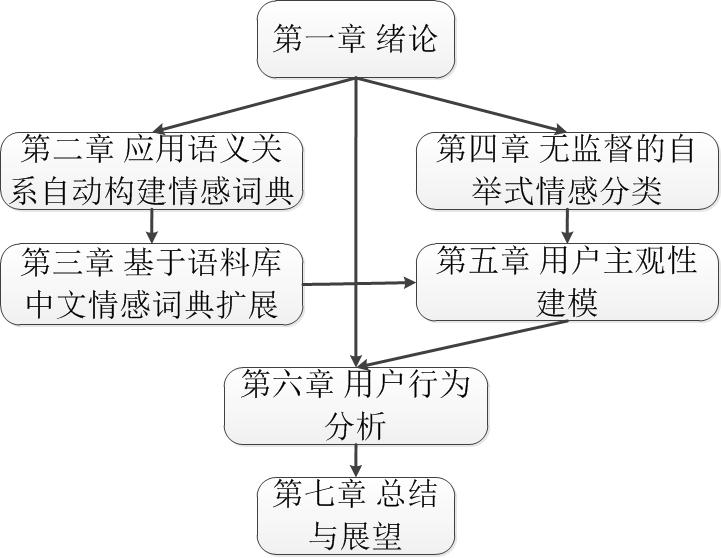
\includegraphics[height=250pt]{1-4.jpg}
\caption{论文整体结构图}
\label{fig1-4}
\end{figure}

第一章是绪论,首先介绍了本文研究的背景,介绍了社交媒体和观点分析一些基础知识,接着提出研究动机,阐明了本文所涉及的科学问题、研究内容,并给出了研究方法,然后分析了研究问题,确立了依托自然语言处理技术与机器学习方法解决这些问题的基本思路,最后介绍了本文的主要工作和文章的结构。

第二章是应用语义关系自动构建中文情感词典,首先介绍了目前情感词典资源的现状,针对中文情感词典资源缺乏问题,提出了以HowNet语义知识库为基础,根据中英文词典语义之间的对应关系将英文情感词典的情感知识转化到中文情感词典中,设计了转化方法以及转化中极性值的计算方法,实验中与现有的几个中文情感词典进行了对比。

第三章是基于语料资源的中文情感词典扩展,是对第一章中构建的通用情感在领域语料中的适应性扩展方法研究,首先介绍了基于语料资源的情感词典构建方法,确定了基于语言特征以及统计特征的扩展方法,并提出了综合使用两种特征的混合特征扩展方法,并分别进行了实验验证。

第四章是无监督的自举式情感分类,本章首先介绍了目前情感分类研究现状,针对领域依赖问题,根据词语在表达情感的不同作用提出了特征空间划分方案,并对研究问题进行了形式化,设计了自举式情感分类框架,选用了三种分类器并进行了实验对比分析。

第五章用户主观性建模,首先定义了社交媒体中用户的观点集成问题,然后提出了主观模型的框架,将用户产生内容中的话题和观点组合进行用户观点集成,并设计了通用的模型构建方法,实验中将主观模型应用到观点预测任务,并对模型进行了定性的分析。

第六章用户的转发行为分析,研究的问题是对于给定一个微博,分析微博作者的粉丝中谁会转发该消息,针对该问题,我们使用主观模型从用户的主观动机角度进行分析,设计了主观相似性计算方法,并针对转发行为的三种情形进行度量,最后在实验中定性和定量验证了我们提出方法的有效性。

最后一章是总结部分,我们阐明了本文工作的贡献点,并且指出了工作的一些不足,并对未来社交媒体中观点信息分析与应用的一些问题和方法进行了尝试性地思考。



\chapter{应用语义关系自动构建情感词典}
\label{ch2}
%本章将进入论文排版的正文, 按元素分主要包括:
%{\kai 字体段落,图片表格,公式定理,参考文献}这几部分。
%这个样例文件将包括模板中使用到的所有格式、模板中自定义命令到或者特有的东西,
%都将被一一介绍,希望大家在排版自己的学位论文前能细致的看一遍,记住样例的格式和
%方法,方便上手。

\section{引言}
\label{ch2:intro}
上一章主要介绍了本文的研究背景,要研究的科学问题,研究内容与方法,并指出观点分析一项基础的工作就是研究如何针对不同应用构建具有足够覆盖面并且良好适应性的情感知识词典。人在使用语言表达情感或观点时,最基本的方式是使用具有明确情感色彩的词汇,因此为了分析用户的观点,最直接的方法应该从用户产生文本中使用的词语开始,将语言中经常使用的词语所表达的情感信息进行汇总形成的词典就是情感词典。观点分析研究首先是在英文文本上开始的,情感词典相关研究也是以英文为主,方法相对比较成熟,形成了一些经常使用的英文情感词典资源。中文情感分析研究起步较晚,缺乏普遍认可的可靠的中文情感词典\upcite{朱嫣岚2006,朱征宇2013,黄硕2013}。目前研究使用主要有HowNet情感词典\upcite{2013},NTUSD情感词典\upcite{Ku2007}以及大连理工大学的情感词汇本体词库\upcite{2013a}。这些词典主要是以手工或半自动方式编辑而成,覆盖度、可靠性和领域适应性受到限制,并且情感知识主要以积极和消极极性二值区分,缺少情感极性值的细粒度划分。能够将资源丰富的英文词典中的情感知识跨语言向中文词典进行适应性的转化,构建相应的中文情感词典资源,既可以省去耗费大量人力的人工标注过程,又可以克服目前中文情感词典自动或半自动构建方法的可靠性和覆盖度问题。
因此本章提出将英文情感词典资源情感知识转化为中文情感词典的构建方法,可以根据语义关系将英文词语及其情感极性值转化得到中文词语的情感极性值,并且完全是自动的,可靠性更高。下一章将该方法构建的情感词典在领域语料中进行扩展,以提高其领域覆盖度和适应性。

本章具体安排如下:首先对情感词典构建需要考虑的问题以及相关工作进行全面的介绍,接着对本章要使用的词典资源进行介绍,然后详细阐述如何利用HowNet双语语义知识库将英文情感词典情感知识转化为中文情感词典相应的词语情感信息,最后对该方法进行实验验证和说明。

\section{相关工作}
构建情感词典需要考虑词典覆盖度(Coverage)、词典内容(Content)以及构建方法(Acquisition)三个方面问题,具体内容可以用图~\ref{fig2-1-1}框架来展示。

\begin{figure}[htp]
\centering
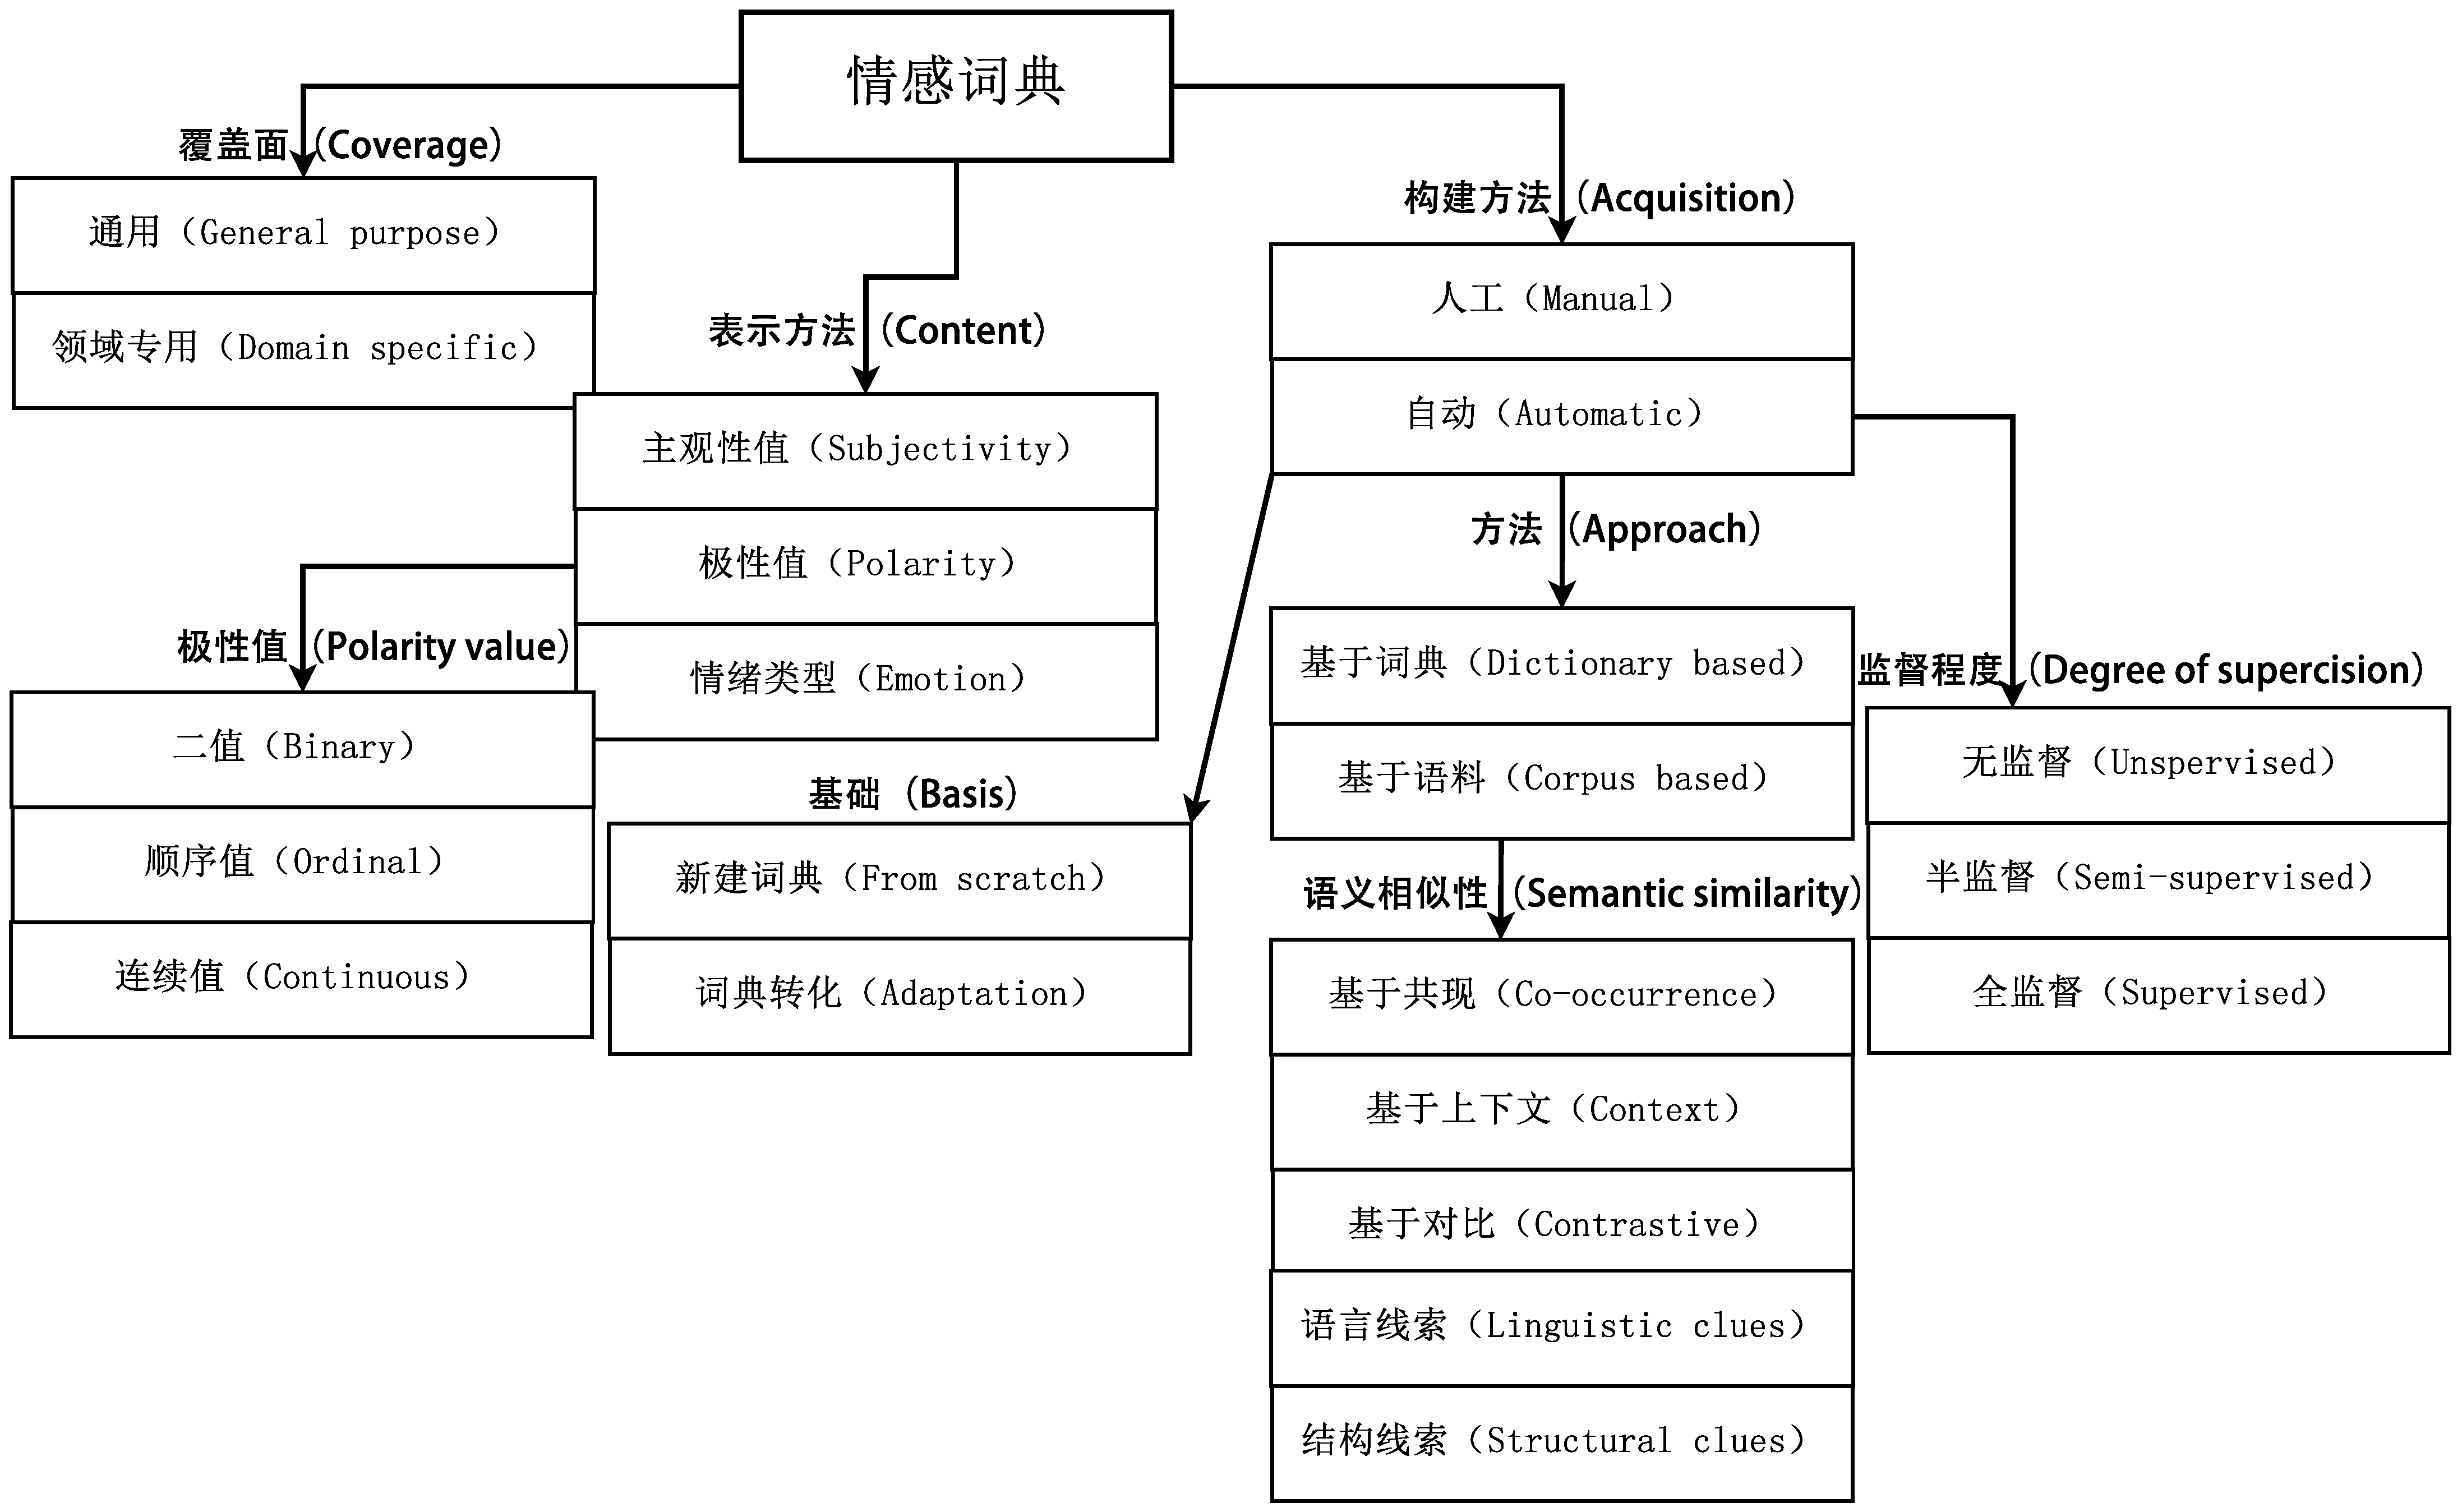
\includegraphics[height=300pt]{2-1-1.eps}
\caption{情感词典相关研究}
\label{fig2-1-1}
\end{figure}

\subsection{词典覆盖面}
就词典的覆盖面来讲,情感词典可以分为通用词典以及领域专用词典。构建通用情感词典的主要假设就是希望词语表达的情感独立于具体的领域和应用,当然这一假设只对一部分词语(比如:“赞”、“爱”、“憎恨”等)是合理的,目前经常使用的情感词典基本都是通用的情感词典。但是实际上很多词语表达的情感是依赖于领域和具体的语境的,比如“轻薄”一词,一般情况表示负面情感,但是描述手机时却可以表示正面的评价。而且,一些本身不表示具体情感的词语(比如:“长”、“短”、“老”、“经典”等),用到一些特殊的语境时也会表达出一些具体情感(比如:“手机待机时间长”与“手机待机时间短”)。因此一些研究开始针对具体领域和应用需求构建一些领域专用的情感词典\upcite{Choi2009,Du2010,Klenner2009}。

\subsection{词典内容}
情感词典可以就其表示情感知识内容进行细分,如果不考虑具体的应用场景,仅对词典的情感表示方法进行划分,情感词典表示情感知识的方法可以分为三种:词语表示主观性的程度(Degree of subjectivity)、表示情感的极性(Polarity)或者表示的情绪类型(Emotion$ / $mood,比如喜、怒、哀、乐等)。表示主观性程度的情感词典主要用于文本主观性的探测任务\upcite{CarmenBanea2008,Gyamfi2009,Maks2012,Wiebe2000,Wiebe2006},而主观文本表达观点的具体情感类型的识别,需要表示情感极性或情绪类型的情感词典。在情感分类中经常使用是表示情感极性的词典,词典中词语条目都标注了表达的情感极性是积极的还是消极的,这些极性知识对于确定文本所表达观点的倾向性是非常重要的。对这类情感词典还可以根据表示的情感极性值进一步划分:比如使用二值情感极性(也就是积极的和消极的)的情感词典\upcite{Godbole2007,Hatzivassiloglou1997,Hu2004,Rao2009};使用顺序值(ordinal)表示极性值的情感词典,比如常使用1-5整数值区分情感极性的强度值\upcite{Yessenalina2011};还有一些使用连续数值(continuous)表示情感极性强度的情感词典\upcite{Turney2003,Sasha2008,Velikovich2010,Remus2010}。
目前有很多这样的英文情感词典,比如:OpinionFinder(OF)\upcite{Wilson2005d},Appraisal Lexicon(AL)\upcite{Taboada2004},SentimentWordNet\upcite{Baccianella2010}以及Q-WordNet\upcite{Agerri2010}等。

如果为了分析更细粒度(fine-grained)的情感,需要将词语表达的情感根据情绪类型进行表示,比如Bollen等\upcite{bollen2011twitter}通过分析Twitter中大量用户表达出的不同情绪来预测股票指数的变化,Garcia和Schweitzer\upcite{Garcia2011}对产品评论中的情绪类型进行了细致研究,类似的工作还有Davidov等\upcite{Davidov2010}以及Strapparava和Mihalcea\upcite{Strapparava2008}在Twitter上的工作。这种类型的情感词典都是靠人工编辑形成的,比如GI(General Inquirer)\footnote{\url{http://www.wjh.harvard.edu/~inquirer/Home.html}}\upcite{Stone1966},ANEW(Affective Norms for English Words)upcite{Bradley1999},WordNet-Affect\footnote{\url{http://wndomains.fbk.eu/wnaffect.html}}upcite{Valitutti2004,Valitutti2004a},DAL (Dictionary of Affect in Language)\upcite{Whissell1989}等词典。

\subsection{词典构建方法}
从情感词典的构建方法来看,可以分为人工构建和自动构建两种类型。目前公开可用的人工编辑的情感词典基本都是通用的情感词典(比如:OF词典和GI词典),人工构建情感词典主要面临的问题除了需要耗费大量的人力,还有覆盖面相对较低,并且需要对不同的领域进行适应性扩展才能达到好的观点分析效果。
对于自动构建情感词典方法,还可以按照方法(Approach)、监督程度(Degree of supervision)和构建基础(Basis)三个维度进行区分。

\subsubsection{构建方法}
情感词典主要的构建方法分为两类:一是基于词典(dictionary-based)方法,根据已有词典的词语之间的语义关系判断词语的情感极性并计算情感极性值;二是基于语料(corpus-based)方法,根据词语在语料中的分布特性推导出情感极性并计算极性值。两类方法共同特点是都需要一个预先标注的种子词集(seed set),然后通过不断迭代计算词语与种子词集词语之间的某种语义相似性,推导词语情感极性值并扩充种子词集,直到收敛。

\paragraph{基于词典方法:}
基于词典的方法通常会使用一个词库(thesaurus)或语义知识库(常用的是WordNet\upcite{Miller1995}),基本的假设是词语间的语义关系可以用来确定词语的情感极性,最常用的语义关系是词语间的同义和反义关系\upcite{Godbole2007,Kim2006,Ahsaee2010}。例如形容词“lovely”会将积极极性通过同义关系传递给“admirable”、“adorable”、“amiable”和“pretty”,反过来会将消极极性传递给反义词语“awful”、“unlovely”和“ugly”。但是这种转换会随着语义距离增加而弱化,比如在WordNet中从“good”到“bad”的同义关系距离长度只有3\upcite{Godbole2007},因此方法设计时需要采取适当措施将语义距离考虑在内\upcite{Godbole2007,Ide2006,Budanitsky2001,Kim2006,Ahsaee2010}。除了同义和反义关系,一些研究提出使用WordNet中的其他语义关系,比如“similarity”,“derived-from”,“pertains-to”,“also-see”或“attribute”等关系\upcite{Esuli2006,Valitutti2004a}。Takamura等\upcite{Takamura2005}以及Andreevskaia等\upcite{Andreevskaia2006}使用了并不直观的下位关系(hyponymy)构建情感词典。还有一些方法通过计算词语在词典中解释的相似性来度量词语间的语义相关性,然后根据这种语义相关性构建情感词典\upcite{Esuli2006,Baccianella2010,Takamura2007}。

\paragraph{基于语料方法:}
和基于词典方法一样,基于语料方法一个基本思想就是通过某种方法度量词语间的语义相关性,然后从带有情感极性标注的种子词集中推导出词语的情感极性。主要度量方法可以分为以下四种:
\begin{itemize}
\item \textbf{基于词语共现方法}:代表性的工作是Turney等\upcite{Turney2002,Turney2003},主要是假设“一个词语的语义倾向性(semantic orientation)\footnote{Turney使用语义倾向性指代词语的情感极性}往往与其共现的词语的语义倾向性相关”,因此他们使用点互信息PMI统计值对词语和种子词集的相关性进行度量,进而推导出词语的情感极性。
\item \textbf{基于上下文方法}:除了直接通过共现来度量两个词语的相关性,在统计语义学还有还有一种常用的方法就是使用词语的上下文信息。在Firth的《Contextual Theory of Meaning》一书中,提出一个基本的假设就是“a word is characterized by the company it keeps”\upcite{Firth1957},指出词语的语义信息是与上下文语境紧密相关的。一些基于语料的情感词典构建方法利用这一假设,提出在相似上下文出现的词语具有相同的情感极性,因此可以从情感极性已知的种子词集推导出上下文信息相同的词语情感极性\upcite{Baron2003,Wiebe2000,Velikovich2010}。
\item \textbf{基于对比方法}:该类方法将词语在前景(foreground)语料和背景(background)语料中的分布特点对比分析,从而进行情感词语的抽取构建情感词典。比如Maks和Vossen\upcite{Maks2012}研究了对数似然和相对频率比抽取情感词构建语情感词典,他们使用报纸新闻以及新闻评论作为主观前景语料,维基百科文本作为客观背景语料。相似的工作还有Stepinski和Mittal\upcite{Stepinski2007}。
\item \textbf{基于语言线索}:前面几种方法单纯依靠语料中统计出的信息,不考虑对文本的深层次语言学特性分析。一些工作认为一些常用的语言模式有助于词语的情感信息的探测。Hatzivassiloglou和McKeown\upcite{Hatzivassiloglou1997}发现一个句子中连词(“and”和“but”)对所连接词语的情感极性具有一定的限制作用,例如出现在“and”两边的词语一般具有相同的极性,而出现在“but”两边的词语一般极性相反,他们利用这种语言规则上的限制从文本语料中抽取并构建情感词典。在产品评论的观点挖掘研究中一些工作扩展了这种基于连词的语言规则,同时考虑句子内和跨句子的连词规则\upcite{Ding2008,Angel,Kanayama2006,Popescu2007}。
\item \textbf{基于结构线索}:代表性的工作是Kaji和Kitsuregawa\upcite{Kaji2006,Kaji2007}的工作,他们利用HTML文档中的结构线索分别抽取情感极性为积极和消极的句子集,从大量HTML文档中抽取出大概500,000主观句子用于训练情感分类器并构建情感词典。
\end{itemize}

\subsection{词典转化}
上述的所有情感词典构建方法都是从零开始(from scratch)构建新的情感词典,最近也有一些方法研究对已有情感词典进行转化,主要是增强通用情感词典的领域适应性或者从单语言情感词典扩展到多语言。通用情感词典进行领域转化方法,主要有Choi和Cardie\upcite{Choi2009}提出的基于线性规划方法,Du等\upcite{Du2010}提出的基于信息理论框架扩展方法以及Qiu等\upcite{Qiu2009}使用语言模式的扩展方法等。Mihalcea等\upcite{Mihalcea2007}提出了基于词典和基于语料的方法将英文情感词典通过翻译转化为其他语言的情感词典。

\subsection{混合方法}
混合方法指的是构建情感词典时同时考虑多种词典和语料资源。例如Hoang等\upcite{Hoang2008}提出使用WordNet的语义关系产生初始情感词典,然后使用从网络语料中获取的统计信息对其进行完善,词典资源和语料资源用一个误差最小化算法(error minimization algorithm)结合起来。Lu等\upcite{Lu2011}提出将与词语相关四种信息组合起来确定情感极性,包括在通用情感词典中的信息,在词库(thesaurus)中的信息,以及在领域文档集中的语言线索和结构线索信息,这四种信息使用一个基于线性规划的优化框架结合起来确定词语的情感极性。

综上所述,目前有很多种构建情感词典方法,以针对英文资源的构建方法研究为主。中文情感词典的构建方法研究还相对较少,基本上是借鉴英文的构建方法,形成的中文情感词典表示的情感知识是简单的二值极性。本章主要研究如何从英文词典进行转化得到中文情感词典,属于词典转化方法,具体的实现方法是借助于双语语义知识库中的语义关系实现这种转化,而不是使用翻译的方式,形成的情感词典能够通过计算将英文情感词典的情感极性值同时转化为中文情感词典的极性值,情感知识更加丰富。

%随着互联网的发展,尤其是社交网络的发展,各种社交媒体的用户发布内容中出现了海量含有用户主观情感色彩的文本数据。针对网络文本的信息处理开始由获得关键词\upcite{Yuan2013}、事件
%\upcite{张辉2013}、话题\upcite{刘健2013} 等事实信息,开始向情感观点等主观信息深入,情感分析便是近年来迅速发展的信息处理技术\upcite{Liu2012}。从数据中提炼出用户的主观信息对于商业情报、舆情分析等具有重要意义。情感分析技术就是对带有情感色彩的主观性文本进行自动推理、分析、归纳的过程,涉及自然语言处理、机器学习、认知科学以及社会心理学等方面的研究\upcite{黄萱菁2011}。


\section{词典资源简介}
\label{ch2:lex}
本节简要介绍要用到的一些词典和知识库资源,主要是针对本章研究相关部分作介绍。
\subsection{HowNet语义知识库}
HowNet是一个以中英文词语所代表的概念为描述对象,揭示概念与概念之间以及概念的属性与属性之间的关系的知识库\upcite{杜飞龙2000}。HowNet两个重要名词是“义原”和“概念”:概念是对词汇语义的一种描述,每一个词可以表达为几个概念\upcite{刘群2002};义原是最小语义单元,用于定义和描述概念。
\subsubsection{义原} 
HowNet设计了大概2200多个义原,这些义原分为几个大类,具体参见表~\ref{tab2-1}。

\begin{table}[htp]
\centering
\caption{HowNet义原分类}
\label{tab2-1}
\begin{threeparttable}
 \begin{tabular}{|l|l|l|l|}
 \hline
 义原&数量& 示例&语义倾向性\tnote{1}\\
 \hline
 Event$ | $事件& 819& blame$ | $埋怨& 一般有倾向性\\
 \hline
Entity$ | $实体& 142& human$ | $人 & 不具倾向性\\
\hline
Attribute$ | $属性& 117 & length$ | $长度 &一般不具倾向性\\
\hline
aValue$ | $属性值& 899 & good$ | $好 &一般有倾向性\\
\hline
Quantity$ | $数量& 3 & rate$ | $比率 & 一般不具倾向性\\
\hline
qValue$ | $数量值& 13 & ufficient$ | $足 & 一般有倾向性\\
\hline
SecondaryFeature$ | $次要特征& 100 & desired$ | $良&一般有倾向性\\
\hline
Semanticroles$ | $语义角色& 90 & StateFin$ | $终状态 & 一般不具倾向性\tnote{2}\\
 \hline
\end{tabular}
\begin{tablenotes}
%  \centering
  \footnotesize
\item[1]语义倾向性即情感极性。
\item[2]虽然语义角色类不具有倾向性,但是代表的语义关系可以影响其他义原的倾向性。
\end{tablenotes}
\end{threeparttable}
\end{table}

表中可以看出,除了事物类、属性类以及数量类义原,其他义原一般都具有情感极性,并且义原都是由中英双语标识,因此可以通过英文标识从英文情感词典中获得其情感极性值。但是有一部分义原的英文标识不是一个单词(比如:FondOf$ | $喜欢,WhileAway$ | $消闲等),无法直接从英文情感词典直接获得情感极性值。实际上义原之间并不是独立的,义原之间存在复杂的关系,HowNet中描述了义原之间的主要的8种关系:上下位关系、同义关系、反义关系、对义关系、属性-宿主关系、部件-整体关系、材料-成品关系、事件-角色关系。义原之间组成的是一个复杂的网状结构,而不是一个简单树状结构。不过,义原关系中最重要关系是上下位关系,义原根据上下位关系形成了如图\ref{fig2-2}树状层次体系,因此可以借助上下位关系树对无法直接转化那部分义原的情感极性值的计算。

\begin{figure}[htp]
\centering
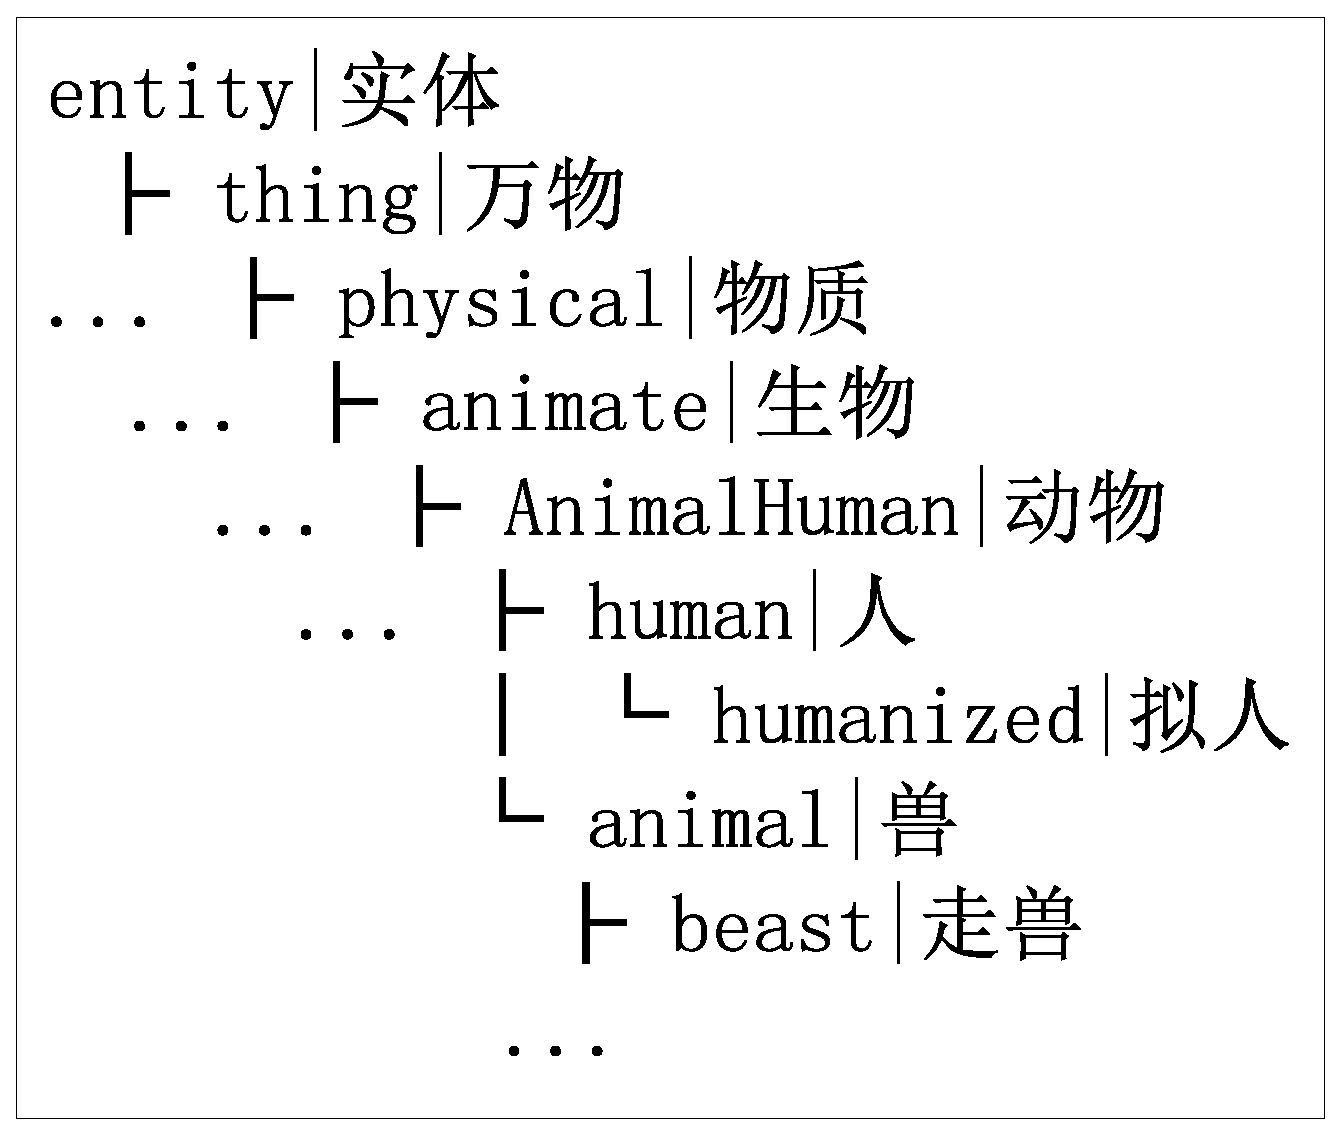
\includegraphics[height=160pt]{2-1-0.eps}
\caption{HowNet义原层次结构}
\label{fig2-2}
\end{figure}

除了义原以外,HowNet还有一些符号(或称为符号义原)对概念语义描述,可以把这些符号归为几类:第一类包括“$ , $”(表示“和”的关系)、“$\sim $”(表示“或”的关系)、“$ \wedge$”(表示“非”的关系),用来表示语义描述式之间的逻辑关系;第二类包括“$\#, \%, \$, \& ,\ast,+,?,!,@ $”,表示概念之间以及概念的属性之间的关系;第三类包括几个无法归入以上两类的特殊符号“$\{\}, \left( \right), \left[ \right]$” 。这些符号义原中第一类描述逻辑关系的三个符号会引起所描述义原情感极性的变化,尤其是“$ \wedge$”会引起情感极性的反转。

\subsubsection{概念}
如图~\ref{fig2-3}所示,HowNet采用KDML(Knowledge Dictionary Mark-up Language)语言描述概念,其中W\_X表示词语,G\_X表示词语词性,E\_X表示词语例子,X为C时表示中文,X为E时表示英文。
%DEF是对于该概念的定义项,称之为一个语义表达式,其中中英文标注的是义原,“\#\*”等标示符号来对概念属性之间关系进行描述,DEF中还可以包含概念,概念之间相互交织构成一个网。HowNet一共有2234个义原,收录了近15万条概念记录,涵盖了绝大部分中文常用词语,本章将基于HowNet的词语进行情感词典的构建。

\begin{figure}[htp]
\centering
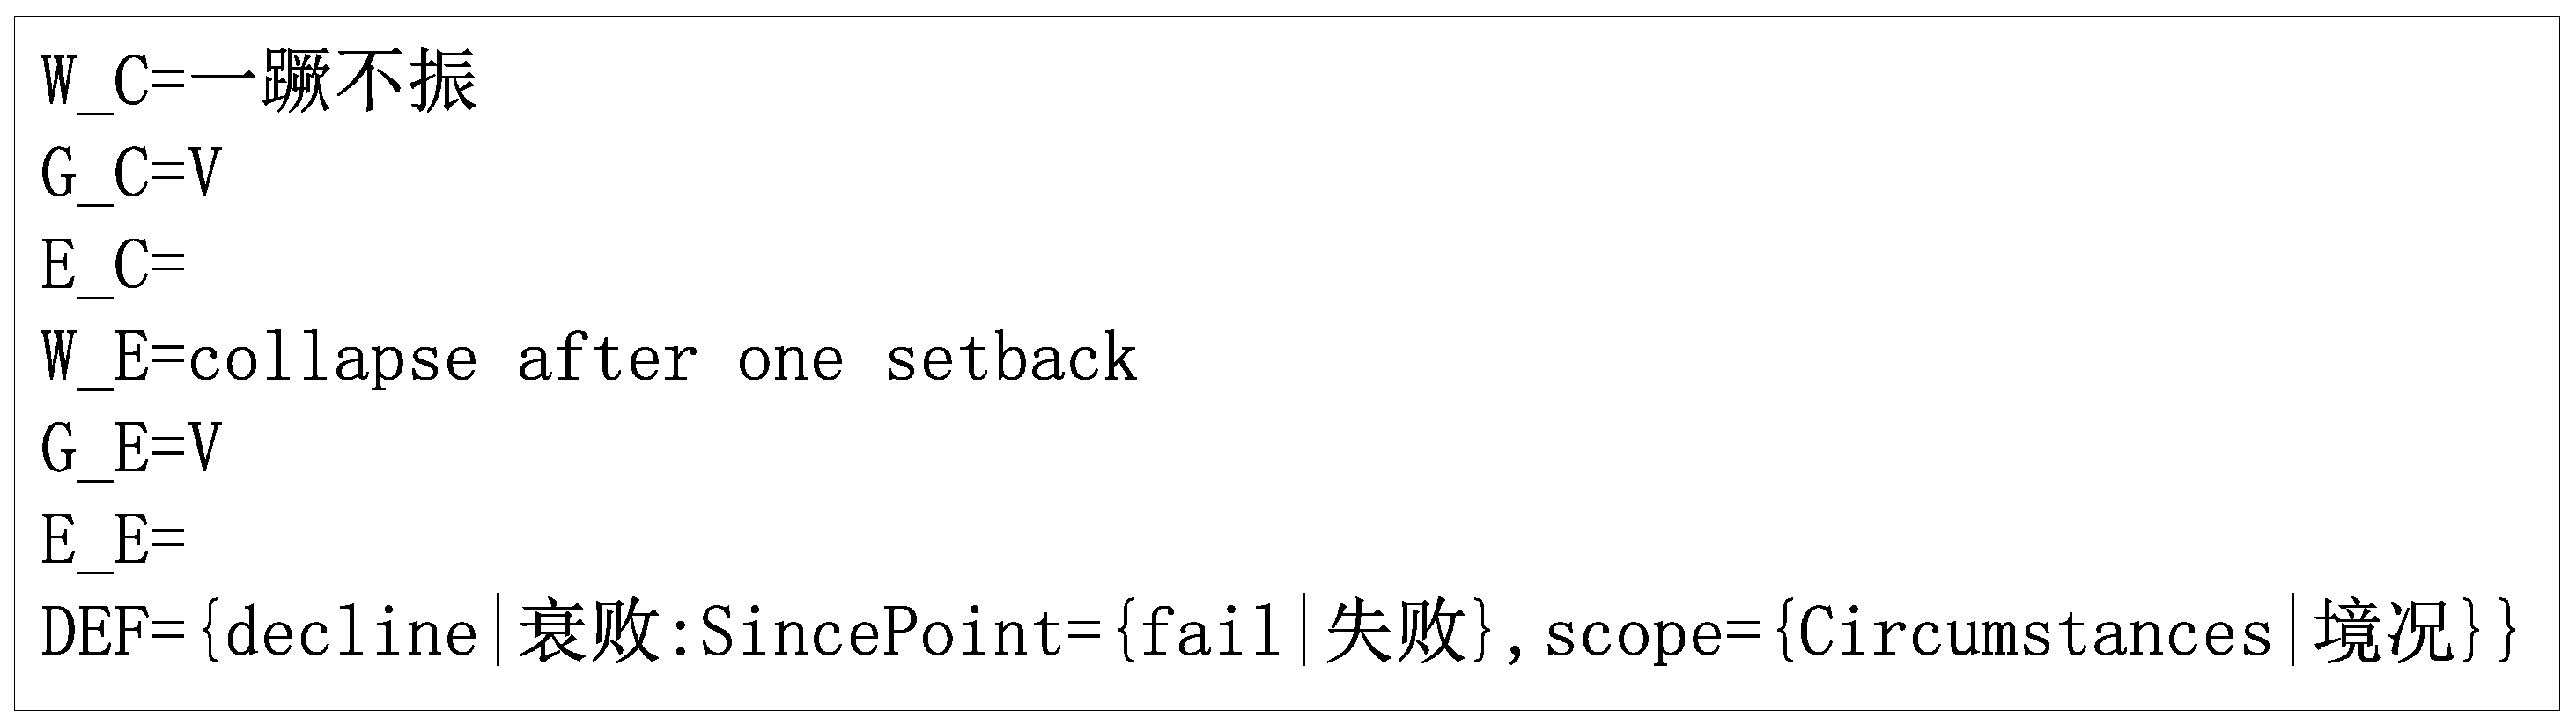
\includegraphics[height=120pt]{2-1-2.eps}
\caption{HowNet中概念描述方式}
\label{fig2-3}
\end{figure}
DEF是HowNet对于概念的定义,称为语义表达式,是知网的核心。HowNet知识描述语言是比较复杂的,为了后续分析计算,在此归纳为以下几条:
\begin{enumerate}
\item HowNet收录词语主有两类,即实词和虚词;
\item 虚词描述比较简单,用“\{句法义原\}”或“\{关系义原\}”进行描述,虚词不具情感极性;
\item 实词的描述就比较复杂了,由一系列用逗号隔开的语义描述式组成,其中语义描述式分为三种形式:
     \begin{enumerate}
     \item 独立义原描述式:用“基本义原”,或“(具体词)”描述;
     \item 关系义原描述式:用“关系义原=基本义原”,或“关系义原=(具体词)”,或“(关系义原=具体词)”描述;
     \item 符号义原描述式:用“关系符号 基本义原”或者“关系符号(具体词)”加以描述;
     \end{enumerate}
\item 实词描述代表了该词的语义知识,因为实词一般具有语义倾向性,因此实词的描述式可以帮助确定语义倾向性。
\end{enumerate}

\subsection{WordNet语义词典}
WordNet是由Princeton大学的心理学家、语言学家和计算机工程师联合设计的一种基于认知语言学的英文词典\upcite{Fellbaum1998}。WordNet是根据词义而不是词形来组织词汇信息。如图~\ref{fig2-2-3}所示,WordNet使用同义词集合(Synset)代表概念,词汇关系在词语之间体现,语义关系在概念之间体现。WordNet将英语的名词、动词、形容词和副词组织为Synsets,每一个Synset表示一个基本的词汇概念,并在这些概念之间建立了包括同义关系(synonymy)、反义关系(antonymy)等多种语义关系,其中最重要的关系就是词的同义反义关系。

\begin{figure}[htp]
\centering
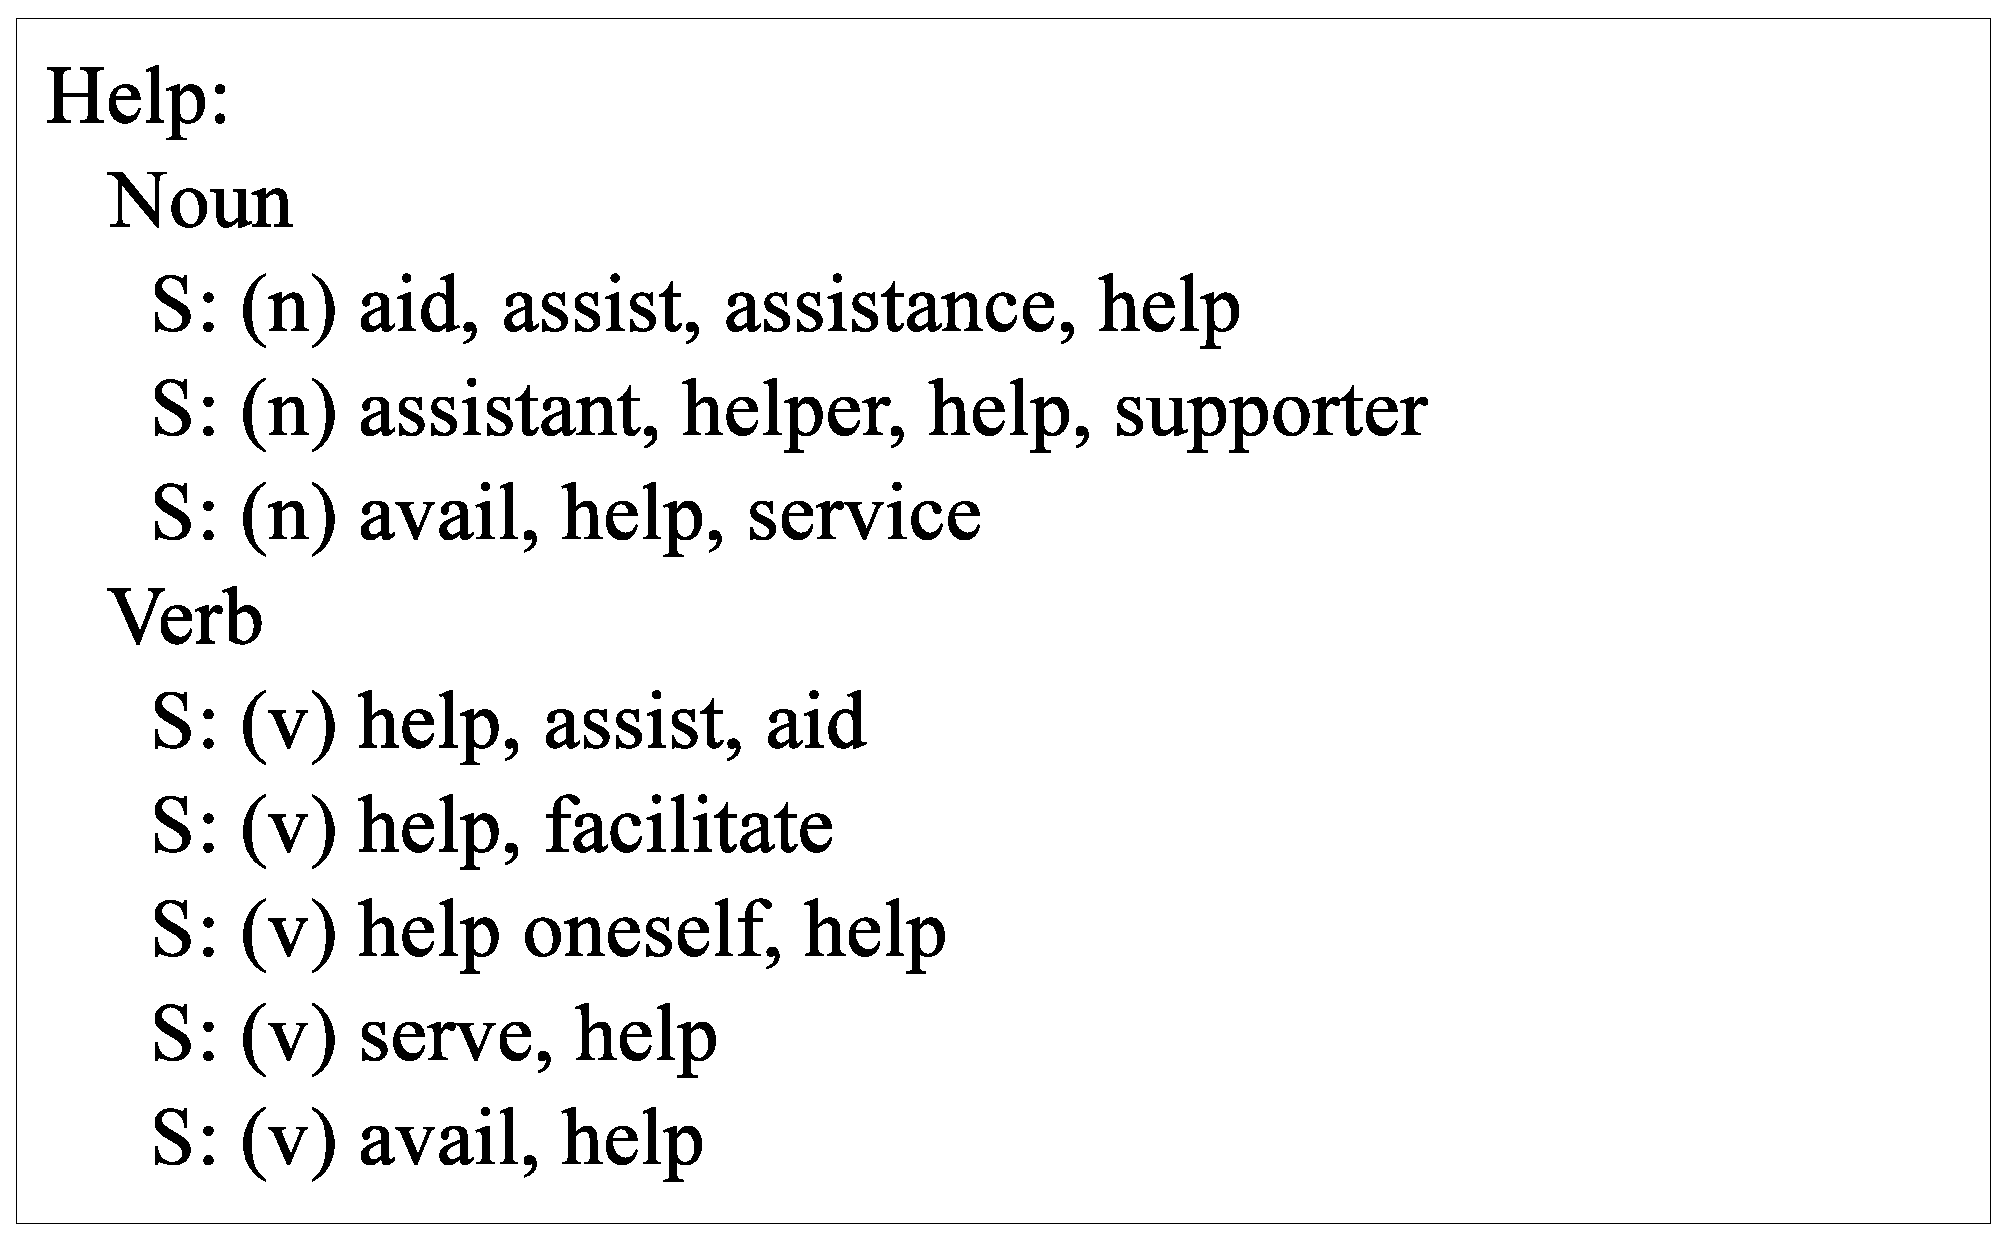
\includegraphics[height=180pt]{2-1-3.eps}
\caption{WordNet单词描述方式}
\label{fig2-2-3}
\end{figure}

\subsection{SentimentWordNet情感词典}
SentimentWordNet是Baccianella\upcite{Baccianella2010}等在语义词典WordNet基础上使用随机游走的图算法计算得到的情感词典。如图~\ref{fig2-2-4}所示,SentimentWordNet的每条记录都是一个WordNet的Synset条目,并且每个Synset都计算出了积极、消极情感极性的强度值(简称情感极性值),本章就是利用SentimentWordNet的情感极性值以及HowNet概念的语义关系进行计算得到中文词语的情感极性值,实现从英文情感词典到中文情感词典的情感知识转化。SentimentWordNet共有收录了117,000多个Synsets,约192,493单词。

\begin{figure}[htp]
\centering
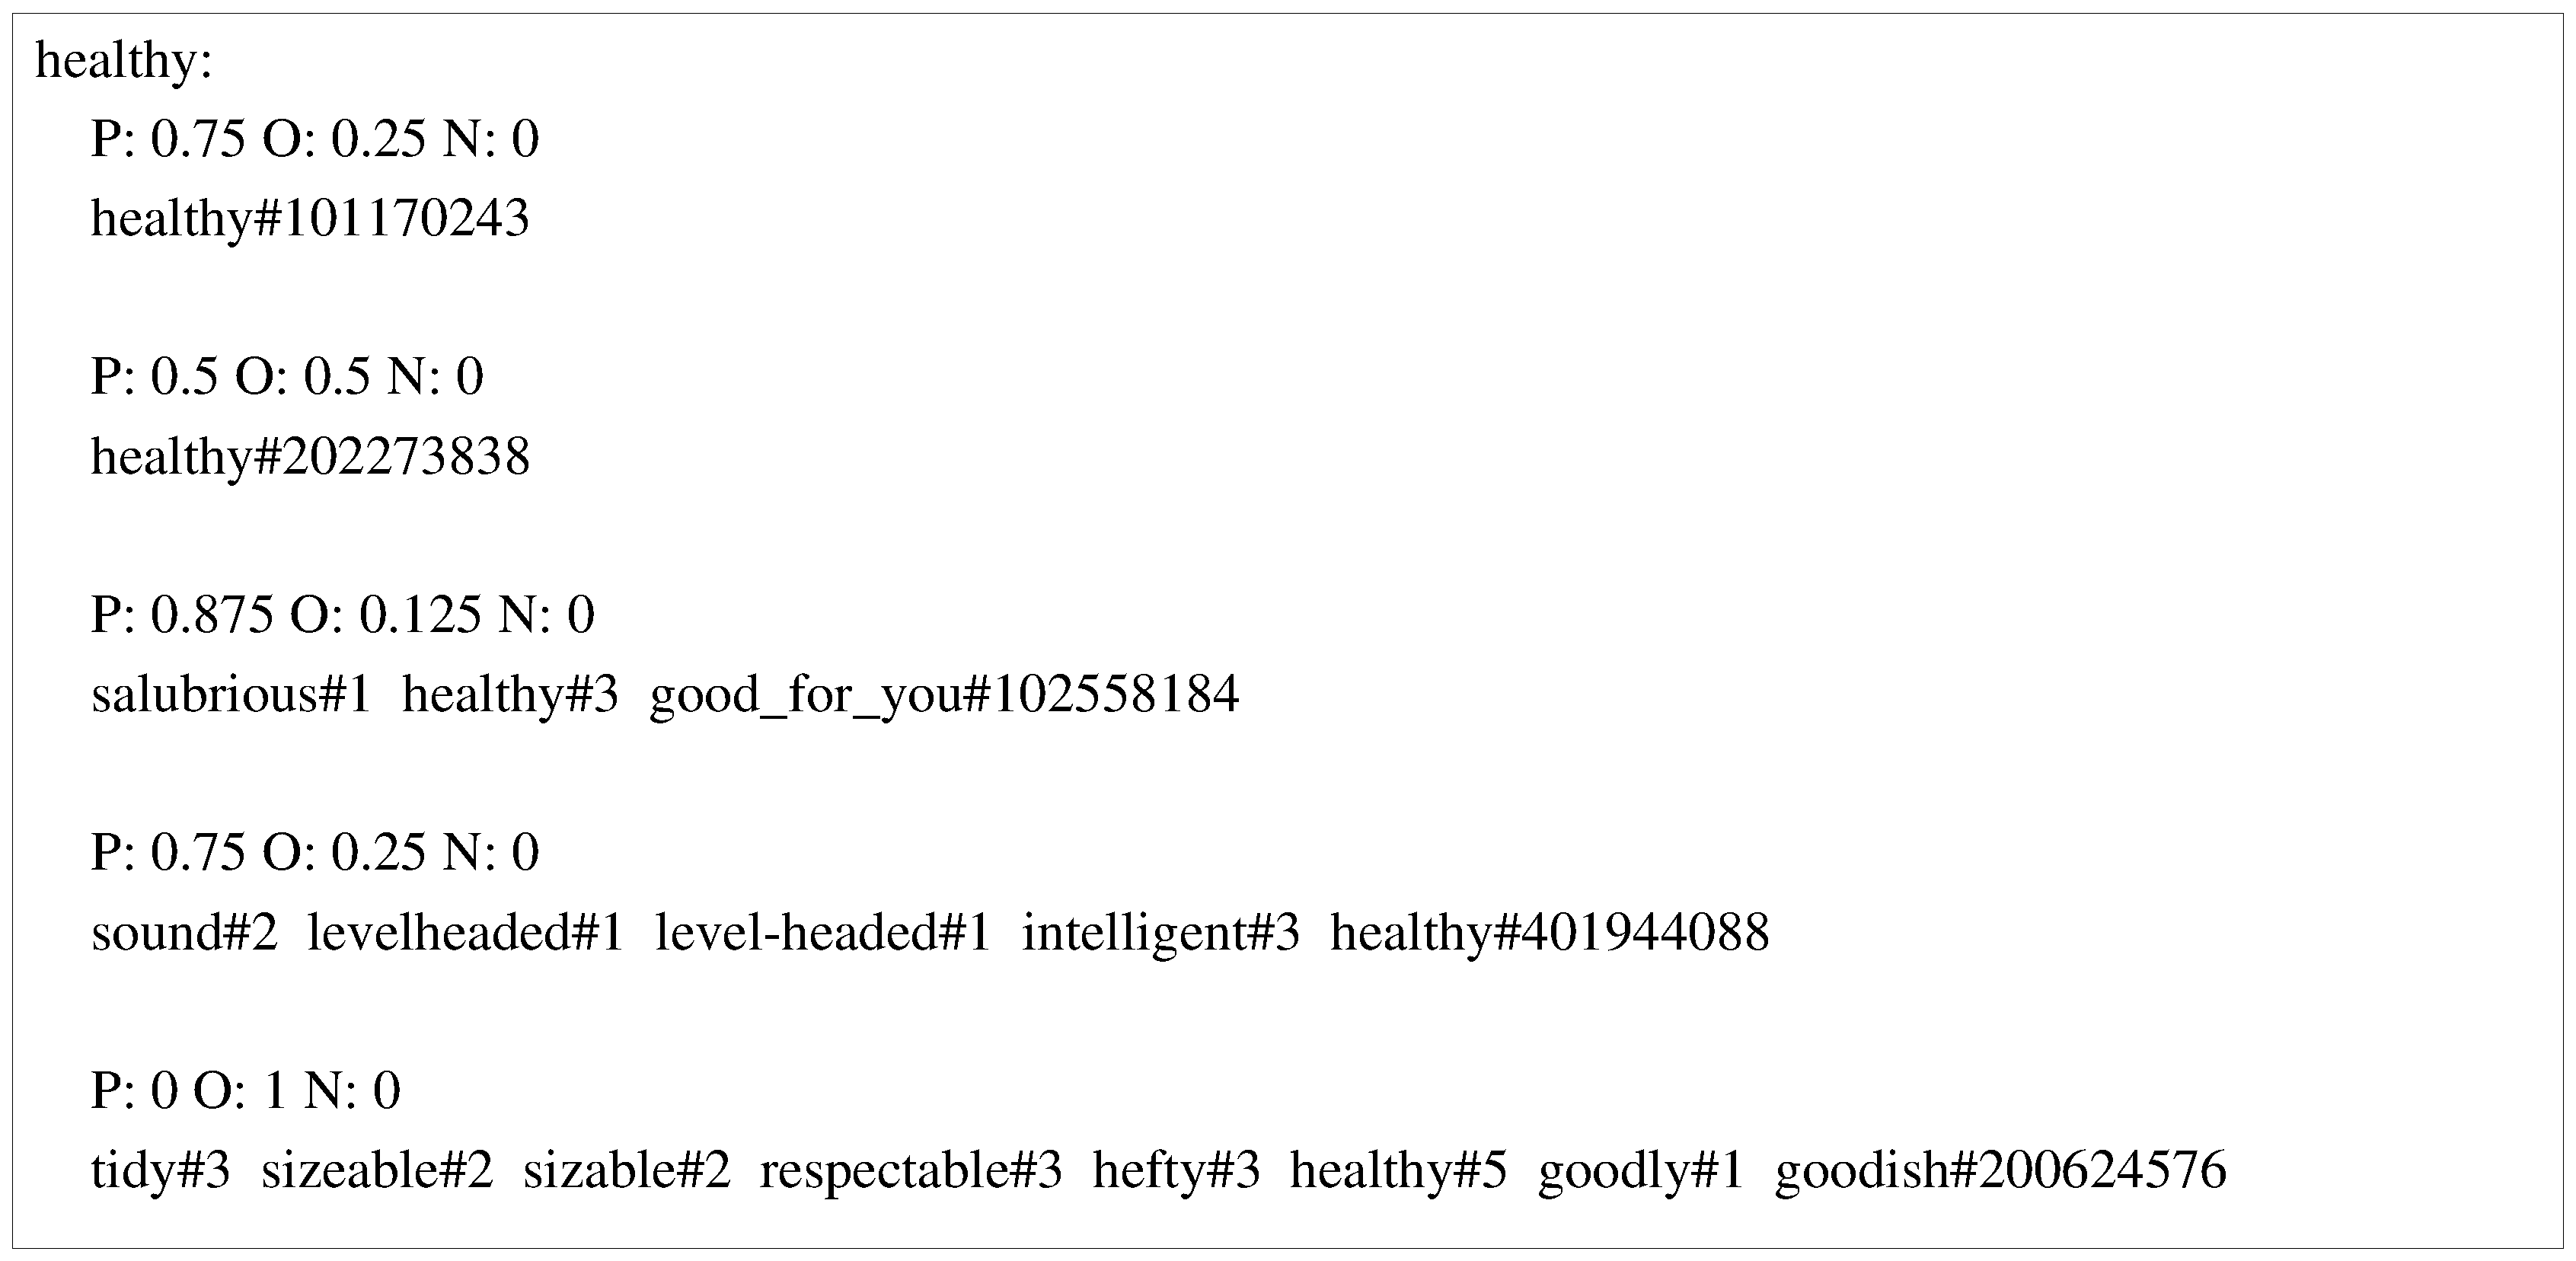
\includegraphics[height=220pt]{2-1-4.eps}
\caption{SentimentWordNet情感词描述方式}
\label{fig2-2-4}
\end{figure}

\section{基于语义关系的情感词典构建方法}
如本章相关工作部分所述,要构建一个新的情感词典有两种方式,一是从零开始(from scratch),另外一种就是通过转化(adaption)其他词典资源的方式。中文观点分析的研究在最近几年才开始受到重视,并且主要是借鉴英文研究已有的资源和方法。中文和英文语法结构和语义表示上存在很大的差别,直接套用英文的资源和研究方法会出现“水土不服”,比如直接将英文情感词典通过翻译方式转化的中文情感词典,是一个从英文情感知识到中文情感知识“给”的方式转化,是将英文情感词典内容映射到中文情感词典,因此存在歧义较大,覆盖度较低以及可靠性不高等问题,并且词典中不可避免存在翻译带来的错误。
本章提出一个从中文到英文情感词典去“取”的方式转化情感知识,是从中文情感词典到英文情感词典的逆映射,因此可以根据中文词语的语义单元选择英文对应语义单元然后转化情感知识,有效避免了歧义,而且不受覆盖度的限制,可靠性也更高。
同时可以直接将英文中对情感极性值的计算结果直接转化为中文词语的情感极性值,减少了计算开销。本章研究正是基于这种动机展开的,提出的解决方案如图~\ref{frame}框架所示。

具体来说,主要使用了双语语义知识库HowNet作为中文情感词语的来源以及对应英文查询词语的来源。HowNet对义原(都有英文标注)和概念(大部分都有英文标注)进行了英汉双语标注,可以作为中英文情感知识转化的“桥梁”。图~\ref{frame}计算框架中,每个词语的情感极性值的计算都是由三部分组成,首先是词语对应的英文标注可以从英文情感词典中查询获得情感极性值,第二部分是词语的语义描述DEF中会有义原的英文标注,也可以查询得到情感极性值,第三部分通过对语义描述DEF的语义关系分析,按照义原在DEF中的语义角色对其情感极性值加权后计算词语的情感极性值。

HowNet中有些词语本身没有英文标注,无法通过查询英文情感词典获得情感极性值。有些词语虽然有英文的标注,但是查询英文情感词典时候会遇到一词多义问题,不同语义对应的情感极性值不尽相同,得到的情感极性值也会因为存在歧义而不准确。还有一些词语标注的英文是多个单词,无法直接得到情感极性值。HowNet中词语的语义由概念表示,每个概念都有对应的语义描述DEF,DEF是由一个到多个义原按语义关系组合在一起的,因此概念在中文中是没有歧义的。本章正是利用了HowNet中概念语义描述部分,分析其中义原以及义原之间的关系,将义原情感极性值组合计算出词语的情感极性值。HowNet中义原是描述语义最基本的单位,可以假设义原的情感极性是确定的,基于此假设通过语义关系组合计算出的情感极性值也应该是确定的,因此可以对词语的情感极性进行“消歧”。

综上所述,本章构建情感词典需要解决的问题如下:
\begin{enumerate}
\item 如何基于英文情感词典计算义原的情感极性值?
\item 如何通过概念的语义描述中的语义关系分析组合计算概念的情感极性值?
\item 最后如何组合以上计算结果确定词语的情感极性值?
\end{enumerate}

针对这的三个问题,本章通过情感词语及义原抽取、义原情感极性值计算、以及词语情感极性值计算三个部分进行阐述。

\begin{landscape}
\begin{figure*}
\centering
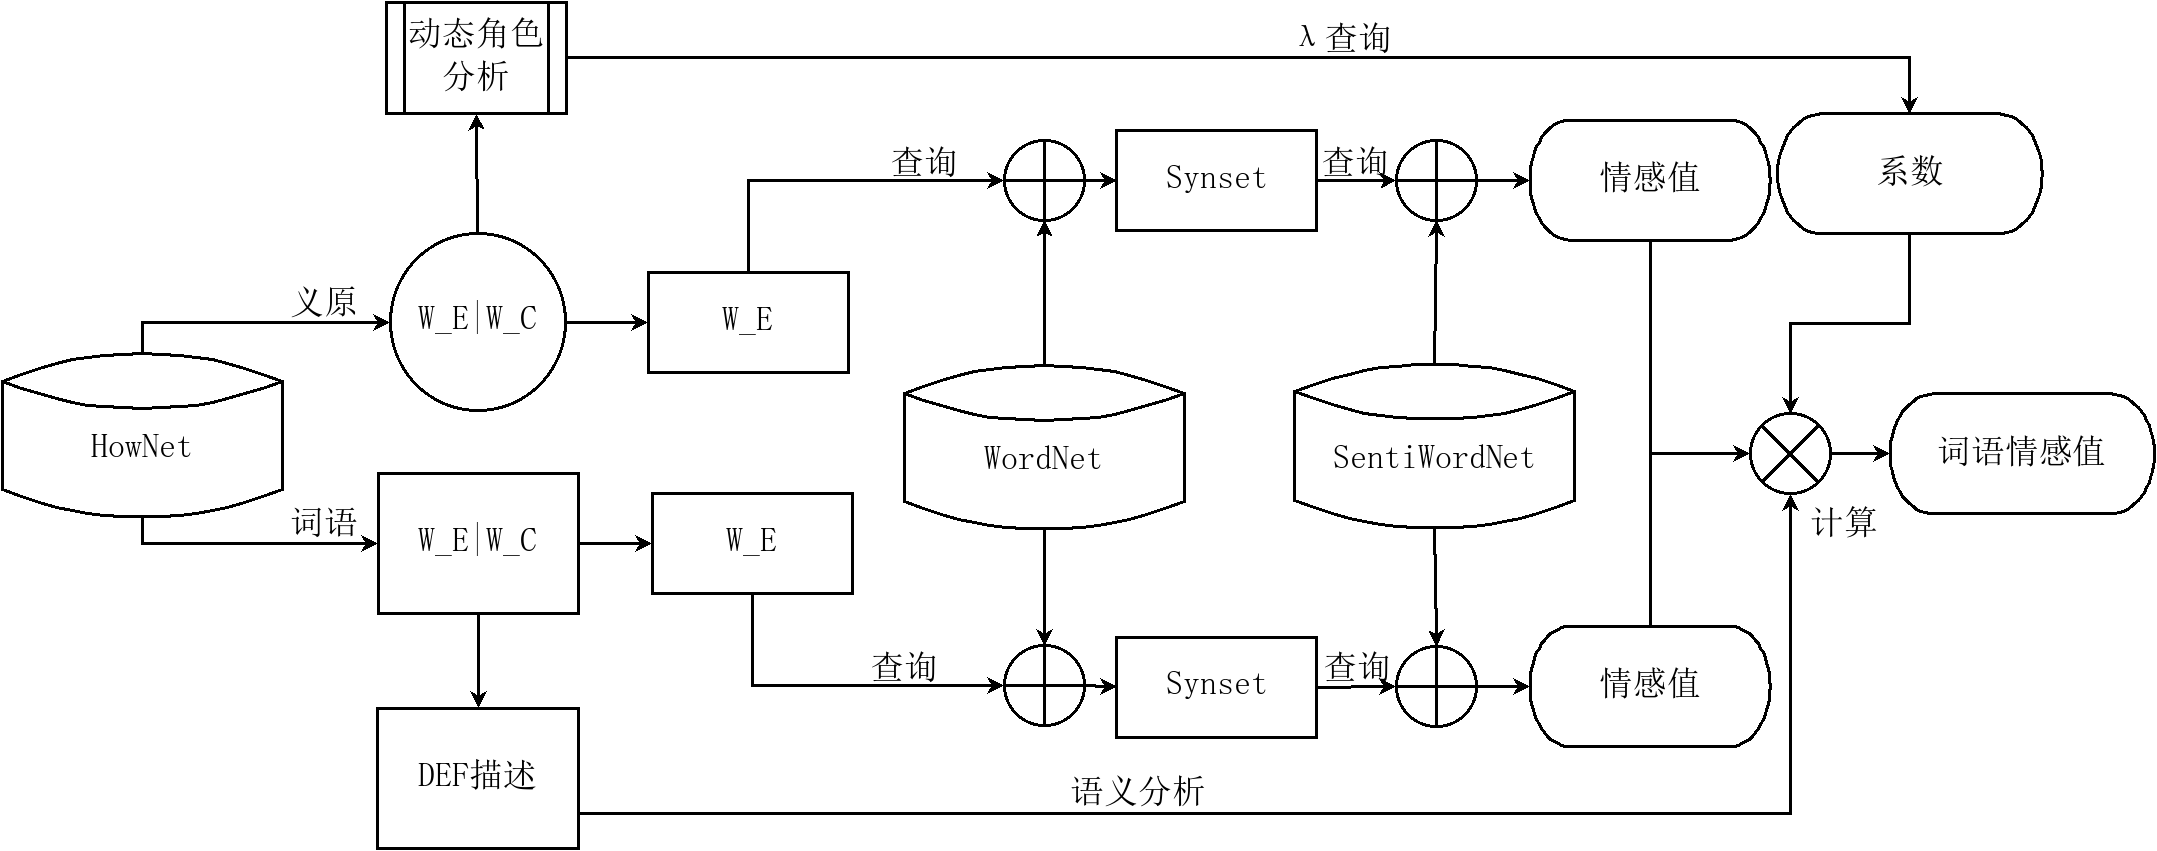
\includegraphics[height=250pt]{2-2.png}
\caption{基于语义关系情感词典构建方案}
\label{frame}
\end{figure*}
\end{landscape}

\subsection{词语和义原抽取}
词语抽取主要是从HowNet中抽取词语(W\_C)和概念描述(DEF),并对DEF进行分析得出其组成义原及语义关系描述符。在进行词语情感极性值计算时,需要根据DEF中义原和语义关系描述符进行词语的语义分析和极性值计算。情感词语和义原抽取处理流程如图~\ref{atom}所示。

\begin{figure}[htp]
\centering
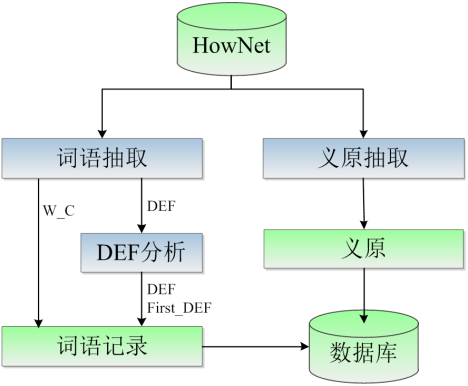
\includegraphics[height=170pt]{2-3.png}
\caption{词语和义原抽取处理流程}
\label{atom}
\end{figure}

从HowNet中抽取出的词语,定义其记录格式如图~\ref{fig2-2-1}所示。
在抽取得到的词语记录中,主要关注的内容有词语编号(No\.)、中文词语(W\_C)、中文词性(G\_C)、英文词语(W\_E)、英文词性(G\_E)、属性(DEF)、第一属性(First\_DEF)等。其中第一属性是指位于属性DEF第一位置的义原,通过第一属性可以分析出该词语所属的特征类。

\begin{figure}[htp]
\centering
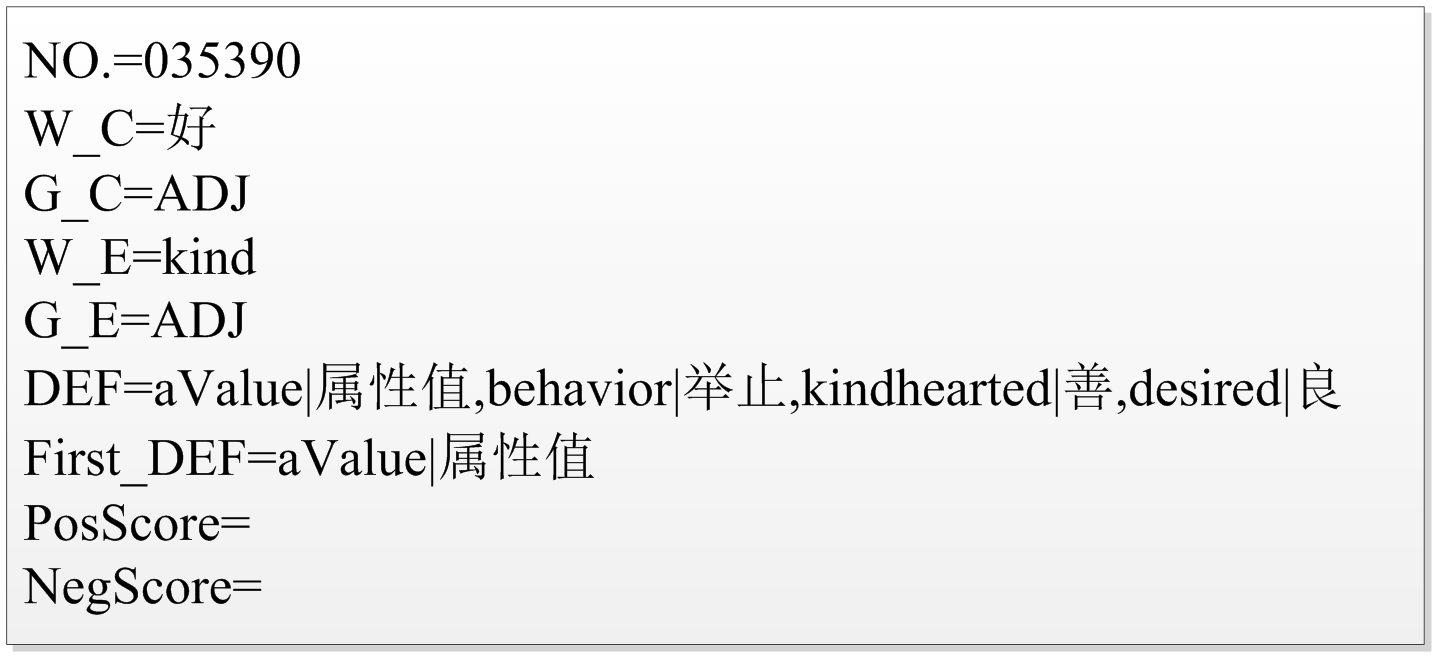
\includegraphics[height=125pt]{2-2-1.png}
\caption{抽取词语记录格式}
\label{fig2-2-1}
\end{figure}

从HowNet中抽取得到的义原的记录格式如图~\ref{fig2-2-2}所示。在抽取得到的义原的记录中,主要关注的内容有词语编号(No\.)、特征类别(Category)、中文词语(W\_C)、英文词语(W\_E)、属性(DEF)、层次(Layer)、父亲节点编号(Father)等。根据记录中的层次(Layer)和父亲节点编号(Father)可以得到义原之间的层次关系,如编号为33的义原“依靠”位于“事件类(Event)”的第五层,其父亲节点编号为32,通过查询编号为32的义原,得到其父亲节点义原为“有关(relate)”。

\begin{figure}[htp]
\centering
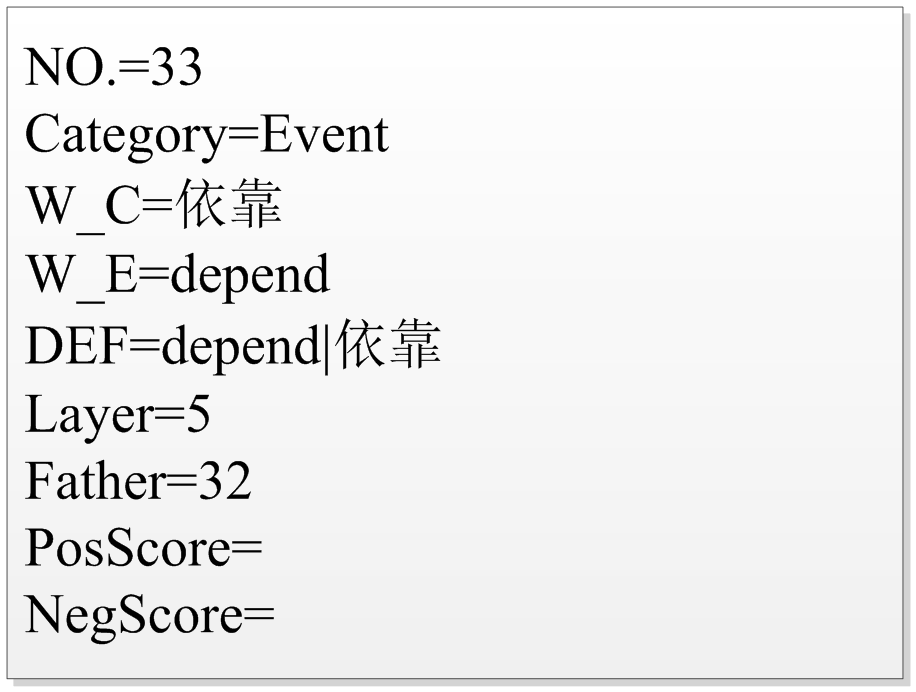
\includegraphics[height=125pt]{2-2-2.png}
\caption{抽取义原记录格式}
\label{fig2-2-2}
\end{figure}

\subsection{义原情感极性值}
在词语情感极性值计算中,义原的情感极性值的确定是非常关键的,是计算词语情感极性值的基础。在HowNet中义原都使用中英双语标注,基本都可以根据英文标注查询得到情感极性值(称为查询类义原极性值)。也有一部分义原英文标注由多个单词连接组成(如“FreeOfCharge$ | $免费”),无法直接查询得到情感极性值,可以通过在上下位关系树中与其他义原的语义距离进行计算获得(称为计算类义原极性值)。最后可以通过义原间的反义和对义关系对计算出的义原情感极性值进行校正。

\subsubsection{查询类义原极性值}
WordNet是以词义(Sense)来记录的,Sense以同一词义的词集Synset表示。通过查询可以得到词语W\_E所有的Sense,将每个Sense映射到SentimentWordNet就可以得到对应的情感极性值。
基于WordNet和SentimentWordNet的义原极性值计算过程如图~\ref{atomsen}所示。

\begin{figure}[htp]
\centering
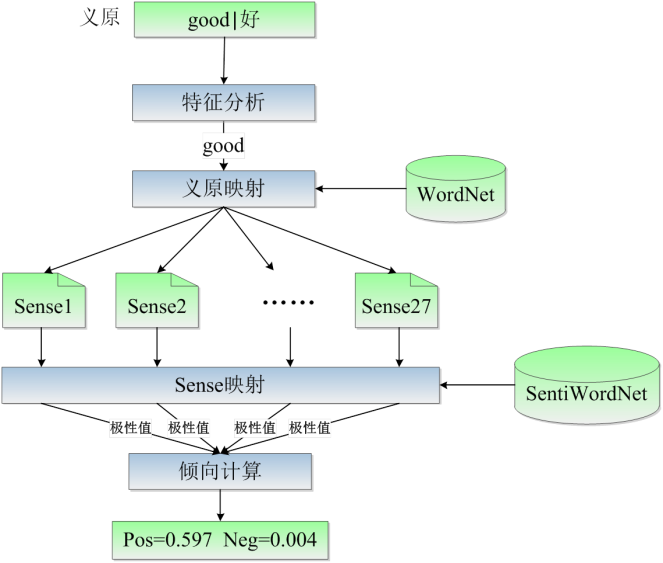
\includegraphics[height=250pt]{2-4.png}
\caption{义原情感极性值计算过程}
\label{atomsen}
\end{figure}

在HowNet中获取义原后将义原对应英文单词(如“good”)映射到WordNet中进行查询,得到该词语所有的Sense(如“good”的Sense共有27个);将这些Sense再映射到SentimentWordNet中查询得到对应Sense情感极性值;将情感极性值加权根据公式~\ref{eq1}计算得到义原的情感极性值(如“good”的极性值为PosScore=0.597,NegScore=0.004)。
\begin{equation}
\label{eq1}
\varphi(s,p)=\dfrac{\sum_{i=1} \varphi_i (s,p)}{\sum_{p\in P}\sum_{i=1}^m \varphi_i(s,p)}
\end{equation}

公式中$ P$表示极性类型(积极(P)和消极(N)),$m$为与义原相对应的Sense的总数,$s$表示义原,$\varphi(s,p)$表示义原的极性值,$\varphi_i (s,p)$表示义原在编号为$ i $的Sense中的$ p $类型极性值。

\subsubsection{计算类义原极性值}
经过上面的查询计算过程,可以得到大部分义原的情感极性值。由于所有的义原根据上下位关系构成了一个树状的义原层次体系,针对一些无法通过查询计算得到情感极性值的义原,可以使用语义距离计算相似度的办法间接计算出情感极性值。假设两个义原(一个情感极性值已知,一个未知)在上下位层次体系中的路径距离为$ d $,根据公式~\ref{eq2-1},可以得到这两个义原之间的语义距离:
\begin{equation}
\label{eq2-1}
sim(s_i,s)=\dfrac{\alpha}{d+\alpha}
\end{equation}
其中$ s_i $是情感极性值已知义原,$ s $表示需要情感极性值计算的义原,$ d $是$ s_i $和$ s $在义原层次体系树中的路径长度。$ \alpha $是一个可调节的参数,一般$ \alpha=0.5 $。

为了能够在上位和下位义原的情感极性值取得平衡,对任意一个情感极性值未知义原$ s $,都要计算$ s $与最靠近$ s $极性值已知的上位义原$ s_1 $ 和下位义原 $ s_2 $之间的语义距离:$sim(s_1,s)$和$sim(s_2,s)$。然后对上位义原$ s_1 $ 和下位义原 $ s_2 $的情感极性值加权平均得到$ s $的情感极性值。
\begin{equation}
\varphi(s,p)=sim(s_1,s)\varphi(s_1,p)+sim(s_2,s)\varphi(s_2,p)
\end{equation}

\subsubsection{情感极性值校正}
所有义原使用前面两种方法计算得到情感极性值会存在一些偏差(bias),有些义原偏差会比较大,甚至计算得到的极性值与义原的真实语义倾向相反(如“FreeOfCharge$ | $免费”义原计算得到极性值为PosScore=0.07,NegScore=0.236),因此需要通过利用HowNet中的其他语义关系对上述计算方法进行校正。在此采用了基于HowNet中对义和反义语义关系进行义原情感极性值校正。对于任一义原$ s $,对义或反义义原为$ \overline{s} $,对$ s $情感极性值修正为:
\begin{equation}
\varphi(s,p)=\dfrac{|\varphi(s,p)-\varphi(\overline{s} ,p)|}{2}
\end{equation}



\subsection{词语情感极性值}
词语情感值可以通过两种途径获得,一是通过词语本身的英文标注直接查询英文情感词典,这种方式并不可靠而且存有歧义;二是根据词语的语义描述DEF中的义原的情感极性值计算得出,这种方式相对可靠,每个义原都有确定的情感极性值,因而不存在歧义。为了计算词语的情感极性值,需要对语义描述DEF中的语义关系进行分析,因为义原间的语义关系会引起义原情感值的反转或者在描述语义倾向时的权重变化。
首先对HowNet中因为DEF的语义关系不同引起的情感极性值变化提出如下定义:
\begin{definition}[情感极性值反转]
义原$s$的$p$极性值$\varphi(s,p)$取反运算是,将$s$的积极极性值和消极极性值互换,过程如公式~\ref{2-2}:
\begin{equation}
\label{2-2}
\overline{\varphi(s,p)}=\varphi(s,q),\quad p,q \in P\&\& p \neq q
\end{equation}
\end{definition}
事件类义原有很多在DEF描述中可以引起情感极性值的变化,比如“DoNot$ | $不做,lose$ | $失去”等相当于句子中的否定词,会引起其他词语情感极性值反转,因此本章从819个事件类义原中挑选了在语义描述中起否定作用的义原称为极性反转语义角色,并加以标记。
\begin{definition}[情感极性值加权]
 $\lambda$因子与义原$s$的$p$极性值的加权运算定义为$\lambda$乘法运算,过程如公式~\ref{2-3}:
\begin{equation}
\label{2-3}
\lambda \times \varphi(s,p) =\begin{cases}
& \lambda \varphi(s,p), \quad  \lambda >0\\
& 0, \quad\quad  \lambda=0\\
&|\lambda|\varphi(s,p), \quad  \lambda <0
\end{cases}
\end{equation}
\end{definition}

公式~\ref{2-3}中$\lambda$取值范围为$ \{-1,0,1\} $,具体值需要根据关系义原描述式中的关系义原(动态角色义原)和符号义原描述式中的符号义原确定。符号义原中只有“$ \wedge$”(表示“非”的关系)会改变语义倾向,因此“$ \wedge$”所修饰的义原在计算中权重为$\lambda=-1$。
HowNet中共有90个动态角色义原,本章分别对每个义原进行了分析,确认了其语义关系角色所确定的基本义原的权重取值$\lambda$。
如词语“扭亏为盈”的DEF描述为“DEF=alter|改变,StateIni=InDebt|亏损,StateFin=earn|赚”,义原“InDebte|亏损”为初始状态(StateIni),“earn|赚”为最终状态(StateFin),经过分析后,StateIni描述的“InDebte|亏损”的$\lambda$取值为0,StateFin描述的“earn|赚”的$\lambda$取值为1。

词语的情感极性值计算总结为公式~\ref{2-4}。其中$\varphi(w,p)$表示词语$w$的$p$极性值,$s_i$表示词语DEF中第$i$个义原,$n$为词语DEF中义原总数。
\begin{equation}
\label{2-4}
\varphi(w,p)=\dfrac{\sum_{i=1}^n\lambda_i\times\varphi(s_i,p)}{\sum_{p\in P}\sum_{i=1}^n\lambda_i\times\varphi(s_i,p)}
\end{equation}
其中:$\sum_{p \in P}\varphi(w,p)=1$。

对于已经通过查询得到情感极性值的词语(有多个英文Sense对应的词语的情感极性值$\varphi(\overline{w},p)$,取所有Sense对应极性值的加和平均),可以和通过语义描述DEF计算得到的极性值加权累加,计算公式为:
\begin{equation}
\Psi(w,p)=\alpha \varphi(w,p)+(1-\alpha)\varphi(\overline{w},p)
\end{equation}
其中$ \alpha \in (0,1)$的取值要考虑那种方式得到的情感极性值更准确,一般将$ \alpha $取大些以反映语义描述DEF对词语语义倾向性的影响更大。

\section{实验}
情感词典的实验评测有两种方法,一是直接评测,将情感词典与人工编辑的或者其他可靠性较高的词典进行对比评测;二是间接评测,将情感词典应用到文本情感分类任务评测其性能。本节使用直接评测的方法。

\subsection{直接评测}
在实验评测时,采用HowNet评价词词典基准。HowNet评价词词典是2007年发布的人工标注的词典,每个词语只标注积极和消极极性,没有准确的情感极性值信息。HowNet评价词词典中情感词共有6497项,其中积极极性词语3436项,消极极性词语3061项。

在此将本章中利用HowNet中的语义关系构建的情感词典命名为SentiHowNet。SentiHowNet的词语都有积极极性值和消极极性值,为了和HowNet评价词词典作对比评测,按照公式~\ref{eq2-5}对SentiHowNet的每个词计算得出一个极性。
\begin{equation}
\label{eq2-5}
Polarity(w)=\begin{cases}
positive \qquad & score(w)>T\\
negative \qquad & score(w)<-T
\end{cases}
\end{equation}
其中$ score(w)= \varphi(w,P)-\varphi(w,N)$为词语$ w $积极极性值与消极极性值相减得到的差值,$ T $为阈值,差值$ score(w)$高于$ T $则词语$ w $情感极性为积极极性,差值$ score(w)$低于$ -T $则词语$ w $情感极性为消极极性。当$ T=0 $时,我们构建的SentiHowNet有积极极性情感词12433项,消极极性情感词11148,词典的整体规模达到23581个条目。

评价指标采用常用宏平均和微平均的精准率(P)、召回率(R)以及F值。
\subsubsection{阈值T的设定}
首先考察不同的阈值$ T $对词典评价指标的影响,以确定一个合理的阈值。
图\ref{fig2-5}为$ T $的不同取值对词典性能指标的影响,实验中将$ T $的值由0逐渐增加,当$ T $大于0.1时性能指标基本没有变化或成下降趋势。从图中可以看出,在$ T=0 $时,虽然召回率最高达到88.58\%,但精准率最低仅有54.40\%,F值仅为67.40\%。当$ T=0.05 $时,精准率提高到77.75\%,有较大提高,召回率仅下降到87.61\%,下降幅度较小,F值提高到82.39\%。当$ T $提高到0.05时性能指标达到最好,因此可以设定$ T $为0.05。

\begin{figure}[htp]
\centering
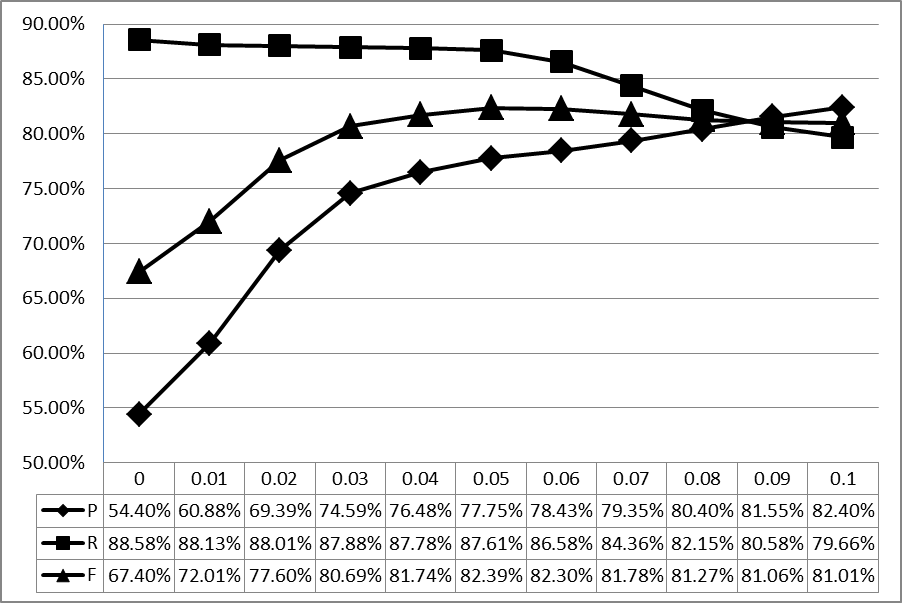
\includegraphics[height=220pt]{2-5.png}
\caption{不同T值时的性能指标}
\label{fig2-5}
\end{figure}

\subsubsection{与其他词典性能对比}
确定了阈值T以后,实验中将SentiHowNet与目前常用的中文情感词典NTUSD词典(11086个中文词汇,2810积极极性词语,8276消极性词语)\upcite{Ku2007}以及大连理工大学的情感词汇本体词库(用DLLEX标记,17156条目,10627个积极极性词语,6529个消极极性词语)\upcite{徐琳宏2008}进行对比评测。首先是三个词典对评价基准词典的覆盖度对比,结果如表~\ref{tab2-2}所示。从表中可以看出,如果按照积极和消极极性分开来看,在积极极性词中SentiHowNet词典覆盖度最好,NTUSD词典由于包含的积极极性词数量少因此覆盖读最低;在消极极性词中,NTUSD词典的覆盖度最好,SentiHownet和DLLEX词典覆盖度基本一样。四种个词典中除了作为基准词典的HowNet评价词词典,采用本章设计方法在HowNet上自动构建的情感词典SentiHowNet包含情感词条目(注意经过阈值T=0.05过滤后)最少,但是对基准词典的覆盖度最高(总体准确标注数达到6092),主要原因是SentiHowNet本身就是从HowNet自动产生,是HowNet包含词语的子集,而NTUSD和DLLEX词典中词语的来源不同,因此会有覆盖度的偏置。

\begin{table}[htp]
\centering
\caption{词典覆盖度}
\label{tab2-2}
\begin{tabular}{|l|l|l|l|l|l|l|}
\hline
\multicolumn{1}{|c|}{\multirow{2}{*}{词典}} & \multicolumn{2}{c|}{积极极性} & \multicolumn{2}{c|}{消极极性} & \multicolumn{2}{c|}{总体统计} \\ \cline{2-7} 
\multicolumn{1}{|c|}{} & \multicolumn{1}{c|}{标注} & \multicolumn{1}{c|}{正确} & \multicolumn{1}{c|}{标注} & \multicolumn{1}{c|}{正确} & \multicolumn{1}{c|}{标注} & \multicolumn{1}{c|}{准确} \\ \hline
HowNet & \multicolumn{2}{c|}{3436} & \multicolumn{2}{c|}{3061} & \multicolumn{2}{c|}{6497} \\ \hline
NTUSD & 2810 & 2204 & 8276 & 3022 & 11086 & 5226 \\ \hline
DLLEX & 10627 & 3020 & 6529 & 2876 & 17156 & 5896 \\ \hline
SentiHownet & 4256 & 3218 & 5113 & 2874 & 9369 & 6092 \\ \hline
\end{tabular}
\end{table}

在T=0.05时,SentiHowNet与其他词典性能比较如表~\ref{tab2-3}所示。在积极极性词语的性能对比中,SentiHowNet词典的精确率和F值最好,分别达到了93.66\%和83.67\%,但是召回率(75.\%61)比NTUSD词典(78.43\%)略差;在消极极性词语的性能对比中,三个词典的精确率都比较高(都超过90\%),但是召回率比较低,NTUSD词典精确率最好,达到98.73\%,而SentiHowNet词典在召回率和F值上性能最好;总体来看,宏平均指标中SentiHowNet词典精准率为93.77\%,召回率为65.02\%,F值为76.79\%,均为三个词典中最高。
\begin{table}[htp]
\centering
\caption{词典性能对比}
\label{tab2-3}
\begin{tabular}{|l|c|c|c|c|c|c|c|c|c|}
\hline
\multicolumn{1}{|c|}{\multirow{2}{*}{词典}} & \multicolumn{3}{c|}{积极极性} & \multicolumn{3}{c|}{消极极性} & \multicolumn{3}{c|}{宏平均} \\ \cline{2-10} 
\multicolumn{1}{|c|}{} & P & R & F & P & R & F & P & R & F \\ \hline
NTUSD & 0.6414 & \textbf{0.7843} & 0.7057 & \textbf{0.9873} & 0.3652 & 0.5331 & 0.8044 & 0.4714 & 0.5944 \\ \hline
DLLEX & 0.8789 & 0.2842 & 0.4295 & 0.9396 & 0.4405 & 0.5998 & 0.9075 & 0.3437 & 0.4985 \\ \hline
SentiHownet & \textbf{0.9366} & 0.7561 & \textbf{0.8367} & 0.9389 & \textbf{0.5621} & \textbf{0.7032} & \textbf{0.9377} & \textbf{0.6502} & \textbf{0.7679} \\ \hline
\end{tabular}
\end{table}

以上两个对比表明相对于需要人工干预的人工或半自动方法构建的情感词典,使用本章设计的自动构建情感词典方法可以构建一部覆盖度比较好,性能又可靠的情感词典,同时节省了不必要的人力开销。

\section{小结}
本章对中文情感词典构建相关研究进行了分类和详细阐述,基于目前中文情感词典研究现状,提出了一种新的跨语言情感词典自动转化方法。该方法以双语语义知识库HowNet、WordNet语义词典和SentimentWordNet情感词典为基础,根据HowNet对词语语义定义和描述的特点,通过双语标注将HowNet义原和词语情感值转换为英文情感词典对应词语的查询与计算。具体来说,中文词语的情感极性值计算被分解为三个部分,分别为义原情感值的计算与校正,词语语义描述的语义关系分析以及最终的词语情感值的计算。按照该方法最终形成情感词典SentiHowNet,词典的规模为:积极极性情感词12433项,消极极性情感词11148项,词典的整体规模达到23581个条目。在实验部分,采用了直接评测的方法,以人工编辑的HowNet评价词典为基准,在覆盖度、精确率、召回率以及F值等指标上与现有的常用情感词典NTUSD和DLLEX词典进行了实验对比。实验结果表明,SentiHowNet对基准词典的覆盖度最好,宏平均的精确率、召回率以及F值最高,证明了该自动构建情感词典方法的有效性,避免了人工和半自动方法的人工干预开销。
\newpage 
\mbox{} 
\newpage
\chapter{基于语料情感词典扩展}
\label{ch3}

\section{引言}
上一章内容主要介绍了进行观点分析的所需的一项基础工作,也就是通用情感词典的构建方法的研究,提出了根据语义词典HowNet语义关系将英文情感词典情感知识跨语言转换为中文情感词典的自动构建方法,并构建了情感极性值标注的中文情感词典SentiHowNet\upcite{谢松县2014}。本章将对通用情感词典SentiHowNet在领域内进行基于语料的扩展,以增加该词典的领域覆盖度和适应性。

%自然语言中,一个词语的语义极性(semantic polarity)表示它对于其语义组(semantic group)或词汇场(lexical field)范式的偏离方向\upcite{Hatzivassiloglou1997}。在自然语言处理领域,情感分析(Sentiment Analysis)能够使用计算手段自动从自然语言中发现观点和情感等主观信息\upcite{Liu2012,Pang2008OMS},通常会使用一些标注了极性(积极或消极)的词汇构成的情感词典资源。研究如何能够通过计算方式获得词语的语义极性,自动构建情感词典一直得到计算语言学和自然语言处理研究人员关注。在英文情感词典构建中,Wilson等\upcite{Wilson2005,Wilson2009}对一些单词进行了人工极性类别的标注形成了OpinionFinder词典;Bradley等\upcite{Bradley1999}标注了并发布了情感范式的英文词典ANEW,后来Nielsen等\upcite{Nielsen2011}在Twitter语言上应用并自动扩展了ANEW,形成AFINN词典。Esuli和Sebastiani\upcite{Esuli2006}以及后来Baccianella等\upcite{Baccianella2010}在著名的语义词典Wordnet基础上采用自动计算的方式开发出了情感词典SentiWordnet。Thelwall等\upcite{Thelwall2012}设计实现了能对词语的情感强度进行估计的方法。情感也可以通过创建情绪词典来进行计算,Plutchik情绪轮提出了四对对立的情绪状态:joy-trust,sadness-anger,surprise-fear和anticipation-disgust\upcite{Plutchik2001}。Mohammad和Turney\upcite{Mohammad2013b}根据Plutchik情绪轮分类方法使用情绪分值标注了一些词语形成NRC情绪词典。在2013和2014年举办的SemEval(Semantic Evaluation)评测中,NRC-Canada队利用NRC词典并扩展出两种新的词典,取得了最好成绩\upcite{Mohammad2013,Kiritchenko2014}。为了克服以上语法层面建立的词典的上下文语境以及领域适应性问题,一些学者提出了基于概念(concept-based)构建情感词典\upcite{Tsai2013},其中SenticNet是使用常识知识库建立的公开可用的基于概念的情感词典\upcite{Cambria2014}。

基于词典的情感词典构建方法是一种常用的情感词典构建方法,采用这种方法的优势在于直接从词典中抽取情感词语,词典中词语间的显式的语义关系也有助于进行情感极性至计算。但是基于词典方法构建情感词典覆盖度受限于词典资源规模,并且只能表示词语通用的情感知识,因而在实际应用中受到多方面的挑战:一方面词典中的词语往往具有多个义项,义项之间的情感极性不尽相同,在实际应用中会存在歧义问题;另一方面,语言的词语本身是开放的集合,会随着人类社会的发展而不断变化,尤其是对于专业领域中不断涌现的新词语,对情感词典在领域内的覆盖度提出了严峻的挑战;还有众所周知的领域适应性问题,也就是相同词语在不同的领域表达出的情感极性也会不一样。这些问题与挑战已经受到越来越多的研究者的注意\upcite{Andreevskaia2008,Choi2009,Du2010,Angel,jijkoun2010generating,Klenner2009,Qiu2009},并且提出了很多基于语料的情感词典构建方法,这些方法已在上一章的相关工作部分进行了详细介绍,在此不再赘述。随着互联网发展,尤其是社交媒体的不断涌现,越来越多的用户在各种网络平台上发布信息,网络上的各种类型用户产生内容(User Generated Content,UGC)包括评论(review)、博客(blogging)、微博(Twitter)以及社交网络的状态(status)等不断涌现并以指数级速度增长。这些类型的UGC中的语言具有不同于传统媒体和知识资源的一些新特点,表达情感的词语数量上达到了新的规模,形式上发生了巨大变化,表达情感极性更加依赖于具体领域和语境,因此研究社交媒体中观点信息需要对在传统知识资源上构建的情感词典进行扩展,提高在UGC数据上的覆盖度以及适应性。
基于这种需求,本章提出并验证基于产品评论语料资源对SentiHowNet情感词典进行领域内无监督的扩展方法。

基于语料资源的情感词典构建方法需要解决两个问题,一是情感词语的选择,就是从语料中确定除了现有情感词典或种子词集以外的带有情感极性的词语,二是对这些词语在语料中表达的情感极性(值)进行计算。在英文中通常将这两个问题合并进行考虑,相关研究主要有两种思路:一是基于语料中文本的语言学线索,代表性研究是Hatzivassiloglou等\upcite{Hatzivassiloglou1997}基于并列或转折连词所连接词语的情感极性制约规律确定新的情感词并判断极性;二是基于语料中词语出现语境中的统计信息,代表性的研究是Turney等\upcite{Turney2002}采用点互信息(PMI)统计语料中与种子词集的词语共现度高的情感词,使用共现统计值并计算其极性值。因此借鉴英文的情感词语选择与极性计算研究方法,本章提出基于中文语料资源对SentiHowNet情感词典扩展的三种方法,并进行实验的验证。
\begin{enumerate}
\item 基于中文语言中的并列、递进以及转折关系的连词进行情感词的发现以及极性值计算方法;
\item 统计词语在语料中上下文信息进行情感词语选择和极性值计算方法;
\item 将基于连词线索方法和上下文信息统计方法相结合的方式进行情感词语选择和极性计算。
\end{enumerate}

本章主要内容介绍采取与上一章不同的结构,首先介绍研究使用的词典和语料资源以及预处理,然后按照方法和实验想结合的方式分别介绍三种情感词典的扩展方法以及实验效果,最后作小节。
\section{数据集及预处理}

\subsubsection{词典和语料}
本章使用的词典和语料资源如表~\ref{tab3-1}所示,选取的语料资源是谭松波博士提供的酒店、书籍和电子商品三个领域评论语料\upcite{Lin2012},每个领域有文本4000篇,其中积极极性评级和消极极性评价各2000篇。
\begin{table}[htp]
\centering
\caption{词典及语料资源}
\label{tab3-1}
\begin{tabular}{|c|l|l|}
\hline
资源 & \multicolumn{1}{c|}{名称} & \multicolumn{1}{c|}{说明} \\ \hline
词典 & SentiHowNet情感词典 & 基于上一章工作 \\ \hline
\multirow{3}{*}{语料} & 酒店(Hotel)评论 & 4000篇,积极评价和消极评价各2000篇 \\ \cline{2-3} 
 & 书籍(Book)评论 & 4000篇,积极评价和消极评价各2000篇 \\ \cline{2-3} 
 & 电脑(NoteBook)评论 & 4000篇,积极评价和消极评价各2000篇 \\ \hline
\end{tabular}
\end{table}

\subsubsection{数据预处理}
对数据的预处理主要包括分词与词性标注以及词语抽取形成结构化记录。
对中文文本进行深入分析前需要进行分词和词性标注,本章直接使用现有的分词工具,也就是广泛使用的中科院ICTCLAS\footnote{目前名字为NLPIR/ICTCLAS,具体见\url{http://ictclas.nlpir.org/}}分词软件\upcite{张华平2014},该工具可以对文本同时进行分词和词性标注。分词和词性标注后,过滤掉一些停用词\footnote{使用哈工大1208词的停用词表进行过滤},语料中所有的词语都有可能成为被扩展对象,因此从语料中抽取出所有词语形成结构化的记录,记录格式如图~\ref{fig3-1}所示,主要内容主要有词语编号(ID)、词性(Category)、中文词语(W\_C)、词语在句子中的编号(Word\_Tag)、词语所在语料文件编号(File\_Tag)、词语所在句子编号(Sentence\_Tag)、极性标注(Senti\_Tag)、积极极性值(PosScore)和消极极性值(NegScore)。值得说明的是,有些词在SentiHowNet中出现过,直接可以通过查询进行极性和极性值标注;极性标注的取值为Yes和No,分别表示已标注和未标注,可以用于在具体的计算过程中直接进行情感词语的选择。

\begin{figure}[htp]
\centering
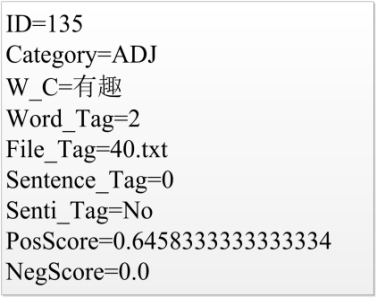
\includegraphics[height=130pt]{3-1.png}
\caption{语料预处理记录格式}
\label{fig3-1}
\end{figure}

\section{基于连词情感词典扩展}
\label{linkage}
Hatzivassiloglou等\upcite{Hatzivassiloglou1997}通过对英文语言的连词在句子中的语法和语义作用研究发现,一个句子中由连词(如and或but)连接的两个形容词或副词的情感极性存在一定的关联性,如并列连词“and”连接的两个形容词(如“nice and good”)情感极性相同,而转折连词“but”连接的两个形容词(如“nice but unnatural”)情感极性相反,否则就会引起语义上的错误(如“nice and unnatural”语法上没有问题,但是语义上存在不正确。)。有研究\upcite{2010}也发现中文语言也会有相同的规律,并且中文连词类型更丰富(有并列、转折、递进、总结、让步等类型的连词),而且数量更多,因此可以选择更多的连词进行情感词的抽取。基于连词的情感词词典构建方法一般只能判断情感词的情感极性,如何能够计算得到情感词的极性强度值需要不同的方法设计。

\subsection{连词选择}
连词是用来连接词与词、词组与词组或句子与句子、表示某种逻辑关系的虚词。连词可以表示并列、承接、转折、因果等关系,对连词上下文的语义倾向性有限制作用的连词一般为并列连词、转折连次以及递进连词。在此主要研究基于表达并列、转折和递进三种关系的连词如何影响情感词的极性值计算,通过筛选选择的连词集合为:
\begin{itemize}
\item \textbf{并列关系连词:}和、跟、与、既、同、及、况、况且、乃至、并、也、又;
\item \textbf{转折关系连词:}却、虽然、但是、然而、偏偏、只是、不过、至于、致、不料、岂知;
\item \textbf{递进关系连词:}不但、不仅、何况、并、且、而且。
\end{itemize}

\subsection{极性值计算}
SentiHowNet情感词典中的每个词都标注了情感极性值,因此语料中未标注的情感词的情感极性值可以根据所有与其在同一句子的SentiHowNet词语情感极性值计算获得。基于连词的情感词语极性计算基本思路是,对抽取到的待标注情感词语(目前之考虑形容词和副词)所在句子进行分析,确定连词及其类型,找到句子中极性值已知的情感词语并分析在句子中与连词和待标注词语的相对位置,然后依据以下原则进行计算:
\begin{enumerate}
\item 位于连词同一侧的形容词或副词具有相同极性;
\item 位于并列连词和递进连词两侧的形容词或副词具有相同极性;
\item 位于转折连词两侧的形容词或副词具有相反极性。
\end{enumerate}
对未标注词的情感值计算,对极性相同的词语情感值累加,极性相反的词语极性值相减,然后取均值。具体情感极性值计算为:
\begin{equation}
\begin{cases}
& PosScore(w_t)=\dfrac{|\sum_{w \in W_1}PosScore(w)+\sum_{w \in W_2}PosScore(w)+\sum_{w \in W_3}PosScore(w)|}{N} \\
& NegScore(w_t)=\dfrac{|\sum_{w \in W_1}NegScore(w)+\sum_{w \in W_2}NegScore(w)+\sum_{w \in W_3}NegScore(w)|}{N}
\end{cases}
\end{equation}
其中,$W_1+W_2+W_3=N$,$N$表示SentiHowNet与待标注词在同一个句子中情感词语,$W_1$,$W_2$和$W_3$分别表示与待标注词$w_t$在连接词同侧词语,在并列或递进连接词两侧词语以及在转折连接词两侧的词语。词语$w_t$极性根据积极与消极极性值大小判定为:
\begin{equation}
\label{eq3-2}
Senti\_tag(w_t)=
\begin{cases}
 positive \quad & \text{ if } PosScore(w_t)> NegScore(w_t); \\ 
 negative \quad &\text{ if } PosScore(w_t)> NegScore(w_t);  \\ 
 neutral  \quad & others
\end{cases}
\end{equation}

情感极性值具体计算过程如算法~\ref{alg3-1}所示。
\begin{algorithm}[htp]
\caption{基于连词的极性值计算}
\label{alg3-1}
\begin{algorithmic}[1]
\REQUIRE ~~\\
待标注词语集$\{w_1\}$;\\
连词集合$\{c\}$;\\
极性值已知词语集合$\{w_2\}$;
\FOR{每一待标注词语 $w_1 \in \{w_1\}$}
\FOR{每一与$\{w_1\}$在同句子中已标注词 $w_2 \in \{w_2\}$}
\IF{$\{w_1\}$和$\{w_2\}$在$c$同侧}
\STATE $
\begin{cases}
PosScore(w_1)+=PosScore(w_2)\\
NegScore(w_1)+=NegScore(w_2)
\end{cases};$
\ELSE
\IF{$c$为并列或递进连词}
\STATE $
\begin{cases}
PosScore(w_1)+=PosScore(w_2)\\
NegScore(w_1)+=NegScore(w_2)
\end{cases};$
\ENDIF
\IF{$c$为转折连词}
\STATE $
\begin{cases}
PosScore(w_1)-=PosScore(w_2)\\
NegScore(w_1)-=NegScore(w_2)
\end{cases};$
\ENDIF
\ENDIF
\ENDFOR
\STATE 计算极性均值$
\begin{cases}
PosScore(w_1)=\dfrac{|PosScore(w_1)|}{N}\\
NegScore(w_1)=\dfrac{|NegScore(w_2)|}{N}
\end{cases};$
\STATE 根据情感值 $PosScore(w_1)$ 与$ NegScore(w_1) $判断极性;
\STATE 将$ w_1 $加入到集合$ \{w_2\} $;
\ENDFOR
\end{algorithmic}
\end{algorithm}

\subsection{实验}
为了评价所提出的基于连词的情感词典扩展方法的性能,从酒店、书籍和电子商品三个领域评论语料中个随机选取了200篇评论(积极和消极极性各100篇)进行了人工标注。标注过程为:首先从评论中抽取其中的形容词和副词,过滤掉SentiHowNet中已有的词语,然后对剩余未标注词语根据在语料中的上下文标注积极和消极情感极性,标注好的词语作为评测基准。
评价指标采用精确率(P)、召回率(R)以及F值(F)作为评测指标。使用基于连词的算法抽取计算并判断极性后,在三个领域扩展得到的情感词数统计如表~\ref{tab3-2}所示。
\begin{table}[htp]
\centering
\caption{情感词典扩展统计}
\label{tab3-2}
\begin{tabular}{|l|l|l|l|l|l|l|l|l|l|}
\hline
\multicolumn{1}{|c|}{\multirow{2}{*}{领域}} & \multicolumn{3}{c|}{积极极性} & \multicolumn{3}{c|}{消极极性} & \multicolumn{3}{c|}{总体统计} \\ \cline{2-10} 
\multicolumn{1}{|c|}{} & \multicolumn{1}{c|}{基准} & \multicolumn{1}{c|}{扩展} & \multicolumn{1}{c|}{正确} & \multicolumn{1}{c|}{基准} & \multicolumn{1}{c|}{扩展} & \multicolumn{1}{c|}{正确} & \multicolumn{1}{c|}{基准} & \multicolumn{1}{c|}{扩展} & \multicolumn{1}{c|}{正确} \\ \hline
Hotel & 103 & 88 & 75 & 98 & 124 & 98 & 201 & 212 & 173 \\ \hline
Book & 166 & 166 & 112 & 245 & 196 & 196 & 411 & 362 & 308 \\ \hline
NoteBook & 61 & 61 & 41 & 66 & 58 & 50 & 127 & 119 & 91 \\ \hline
\end{tabular}
\end{table}

从表中可以看出,在书籍领域扩展得到的情感词语较多,主要是因为书籍的评论篇幅较长,而且有更丰富的词汇来表达对书籍内容的评论,基于连词的扩展方法在消极极性词语的判断准确性较高;电子产品领域扩展的情感词较少,主要是因为对电子产品评论一般较短,表示评价观点的词汇相对比较少,专业化程度更高些,基于连词的极性计算和判断方法在该领域的准确性都比较低;而对于酒店领域基于连词的极性计算和判断方法在该领域的准确性最好。

针对三个领域的情感词典扩展实验性能评测结果如表~\ref{tab3-2-1}所示,三个语料中与上面统计相对应,基于连词的极性计算方法在酒店领域的性能最好,无论是微平均还是宏平均,精确性都高于72.82\%,在消极极性的词语精确率甚至达到100\%,召回率都高于79.03\%,F值都高于78.53\%;电子产品领域的性能指标相对较低,宏平均和微平均三个性能指标较低;在书籍领域,对消极极性情感词的判断召回率达到100\%,精确率以及F值在三个领域中都是较高,总体性能居中。总体来看,基于连词的方法能够对情感词典进行有效扩展,性能较好。
\begin{table}[htp]
\centering
\caption{性能评测结果}
\label{tab3-2-1}
\begin{tabular}{|l|l|l|l|l|l|l|l|l|l|}
\hline
\multicolumn{1}{|c|}{\multirow{2}{*}{领域}} & \multicolumn{3}{c|}{积极极性} & \multicolumn{3}{c|}{消极极性} & \multicolumn{3}{c|}{宏平均} \\ \cline{2-10} 
\multicolumn{1}{|c|}{} & \multicolumn{1}{c|}{P} & \multicolumn{1}{c|}{R} & \multicolumn{1}{c|}{F} & \multicolumn{1}{c|}{P} & \multicolumn{1}{c|}{R} & \multicolumn{1}{c|}{F} & \multicolumn{1}{c|}{P} & \multicolumn{1}{c|}{R} & \multicolumn{1}{c|}{F} \\ \hline
Hotel & 0.7282 & 0.8523 & 0.7853 & 1.0000 & 0.7903 & 0.8829 & 0.8607 & 0.8160 & 0.8378 \\ \hline
Book & 0.6747 & 0.6747 & 0.6747 & 0.8000 & 1.0000 & 0.8889 & 0.7494 & 0.8508 & 0.7969 \\ \hline
NoteBook & 0.6721 & 0.6721 & 0.6721 & 0.7576 & 0.8621 & 0.8065 & 0.7165 & 0.7647 & 0.7398 \\ \hline
\end{tabular}
\end{table}

\section{基于上下文情感词典扩展}
词语的上下文是词语在实际应用中的语言环境,对于词语的语义理解有着重要作用,是自然语言处理经常使用的信息,它在自然语言处理中的价值体现在两个方面:一方面,在自然语言知识获取的过程中,上下文是知识获取的来源;另一方面,在自然语言处理的具体应用问题解决过程中,上下文扮演着问题所需信息和资源提供者的重要角色。特别是在语料库语言学中,各种机器学习方法的引入使词语的上下文成为计算语言学知识获取和问题求解过程中最为重要的资源,在无监督学习方法中更是如此\upcite{鲁松2001}。对于本章要解决的情感词语抽取和极性值计算任务来说,统计情感词语出现的上下文特征可以为情感极性值的计算提供有用信息,因为出现在相似上下文环境中的词语具有相似的极性。

上下文的选取时基于核心词左右一定范围进行的,这个固定的范围被称为“窗口”。选择合适的窗口,可以使得上下文的计算提供的信息量足够大,产生的噪声足够小。在英文中,核心词左右5个词的范围可以为词语搭配提供95\%的信息,上下文±2是最好的选择,范围进一步扩大后提供的信息量不会有明显的增加且会带来不必要的计算开销\upcite{Yarowsky1993,Martin1983}。

词语的上下文可以利用的信息有很多,一般是直接将上下文中出现的词作为有用特征使用\upcite{Sinclair1991,张猛2008},但是这种方法需要面临的一个问题是上下文特征的稀疏性,尤其是对社交媒体文本来说,篇幅一般较短,而且词语的不规范使用现象普遍,稀疏问题会更严重。因此我们采用了上下文词语的词性信息进行统计和计算。具体来讲,首先是对待标注情感词语,分析其上下文中词语的词性,获取一个词性特征向量,然后根据其上下文特征向量进行情感词语极性计算。

\subsection{上下文特征向量}
对于词语$w$,通过分析在一定窗口范围内上下文中词语的词性形成词语的特征向量,下面给出形式化定义。
\begin{definition}[词语$w$的特征向量$V(w)$和窗口$W$]
词语$w$的特征向量$V(w)$是指由词语$w$与其相邻上下文词语的词性组成的向量,具体形式为:
$$V(w)=<C_{-W},C_{-W+1},\cdots C_{-1},C_0,C_{W-1},C_W>$$
其中,$C_0$表示词语$w$的词性,$C_i(i\neq 0)$表示与$w$相邻的词语的词性,$i$表示与词语$w$的相对距离,$W$表示窗口,即特征向量中与词语$w$相对距离的最大值。
\end{definition}

\subsection{基于词性特征向量的情感词极性值}
基于上下文的情感词极性值计算的一个假设就是具有相同的上下文特征向量的词语具有相同的极性,根据这一假设,统计出SentiHowNet中与待标注词$ w_t$词性特征向量相同的情感词,然后计算$ w_t $的情感极性值。如果待标注词$ w_t$出现的上下文中有$ N $中词性特征向量,则$ w_t$的情感极性值计算公式为:
\begin{equation}
\label{eq3-2-1}
\begin{cases}
PosScore(w_t)=\dfrac{\sum_{V(w)=V(w_t)}\dfrac{|\sum_{w \in W_{positive}}PosScore(w)-\sum_{w \in W_{negative}}PosScore(w)|}{|M|}}{|N|} \\
NegScore(w_t)=\dfrac{\sum_{V(w)=V(w_t)}\dfrac{|\sum_{w \in W_{positive}}NegScore(w)-\sum_{w \in W_{negative}}NegScore(w)|}{|M|}}{|N|} \\
\end{cases}
\end{equation}
其中$W_{positive}+W_{negative}=M$,表示与待标注词$w_t$具有同一特征向量$ V(w_t) $的SentiHowNet中的情感词集,$W_{positive}$和$W_{negative}$分别为极性为积极和消极的词语。$w_t$极性判断依据其积极与消极极性值的大小判断,同公式~\ref{eq3-2}。

以书籍语料中形容词“亮丽”为例,设定$ W=2 $,在语料中抽取“亮丽”所有的$ N $种词性特征向量,其中的一个的特征向量为$ <daaun> $,从SentiHowNet中获取与“亮丽”的这一词性特征向量相同的所有情感词如表~\ref{tab3-3-1}所示,共有16个情感词与“亮丽”有相同的词性特征向量$ <daaun> $,其中积极极性词语10个,消极极性词语5个,于是可以使用公式~\ref{eq3-2-1}计算其情感极性值为积极极性值为0.4297,消极极性值0.0421。当然这是词性特征向量$ <daaun> $计算出的极性值,将所有$ N $种词性特征向量下计算的极性值取平均就可以得到“亮丽”在书籍领域最终情感极性值。
\begin{table}[htp]
\centering
\caption{计算示例}
\label{tab3-3-1}
\begin{tabular}{|l|l|l|l|}
\hline
\multicolumn{1}{|c|}{情感词} & \multicolumn{1}{c|}{情感词上下文} & \multicolumn{1}{c|}{情感词} & \multicolumn{1}{c|}{情感词上下文} \\ \hline
大 & 没有多大的可读性 & 弱小 & 再贫困弱小的人 \\ \hline
简单 & 太浅显简单的东西 & 有趣 & 又生动有趣的绘画 \\ \hline
真实 & 比较客观真实的角度 & 直观 & 没有明显直观的效益 \\ \hline
新鲜 & 更多新鲜的元素 & 奇妙 & 更多奇妙的东西 \\ \hline
严格 & 太多严格的界限 & 好 & 更多好的作品 \\ \hline
石破天惊 & 颇多石破天惊之语 & 肮脏 & 太多肮脏的东西 \\ \hline
柔软 & 最脆弱柔软的心脏 & 多 & 反正好多的故事 \\ \hline
粗俗 & 原本低级粗俗的俚语 & 曲折 & 明明惊险曲折的战争 \\ \hline
\end{tabular}
\end{table}

更一般的,基于词性特征向量的情感极性值具体计算过程如算法~\ref{alg3-2}所示。

\begin{algorithm}[htp]
\caption{基于统计特征的极性计算}
\label{alg3-2}
\begin{algorithmic}[1]
\REQUIRE ~~\\
待标注词语集$\{w_1\}$;\\
极性已知词语集合$\{w_2\}$;\\
每个词特征向量集合$\{V(w)|w \in \{w_1\}\cup \{w_2\} \}$;
\FOR{每一待标注词语 $w_1 \in \{w_1\}$}
\FOR{$w_1$每一特征向量$V(w_1)$}
\FOR{每一与$V(w_1)  $相同的特征向量$ \{V(w_1)=V(w_2)|w_2 \in \{w_2\} \}$}
\IF{$Senti_Tag(w_2)=positive$}
\STATE $
\begin{cases}
PosScore(w_1)+=PosScore(w_2)\\
NegScore(w_1)+=NegScore(w_2)
\end{cases};$
\ELSE
\STATE $
\begin{cases}
PosScore(w_1)-=PosScore(w_2)\\
NegScore(w_1)-=NegScore(w_2)
\end{cases};$
\ENDIF
\ENDFOR
\STATE 对各个特征向量下的情感值累加
\STATE $
\begin{cases}
PosScore(w_1)+=PosScore(w_1)\\
NegScore(w_1)+=NegScore(w_1)
\end{cases};$
\ENDFOR
\STATE 计算极性均值$
\begin{cases}
PosScore(w_1)=\dfrac{PosScore(w_1)}{i}\\
NegScore(w_1)=\dfrac{NegScore(w_2)}{i}
\end{cases};$
\STATE 根据情感值 $PosScore(w_1)$ 与$ NegScore(w_1) $判断极性;
\STATE 将$ w_1 $加入到集合$ \{w_2\} $;
\ENDFOR
\end{algorithmic}
\end{algorithm}

\subsection{实验}
评测实验使用的数据、基准与评测指标与基于连词的方法~\ref{linkage}节相同。
对三个领域的情感词典扩展实验结果如图~\ref{fig3-2}、图~\ref{fig3-3}和图~\ref{fig3-4}所示,三个图中分别显示了精确率、召回率以及F值的积极和消极极性的宏平均结果。图中可以看出当窗口$W=1$时,在三个领域的数据中,基于词性特征向量方法都能够准确抽取所有的情感词,因此精确率、召回率以及F值相同,分别为67.65\%、72.89\%和72.13\%;当窗口增加到$W=2$时,召回率都略有上升,精确率都有所下降,酒店领域基本不变,书籍领域下降6.62\%,电子产品领域下降最多(8.1\%),F值都变化不大;当窗口增加到$W=3$时,除酒店领域的召回率上升外,其他两个领域和其他指标都出现明显下降。因此通过分析各个领域的性能指标,采用上下文窗口$W=2$时,基于词性特征向量的情感值计算方法性能最好,这与在英文领域的研究结论\upcite{Yarowsky1993,Martin1983}是一致的。

\begin{figure}[htp]
\centering
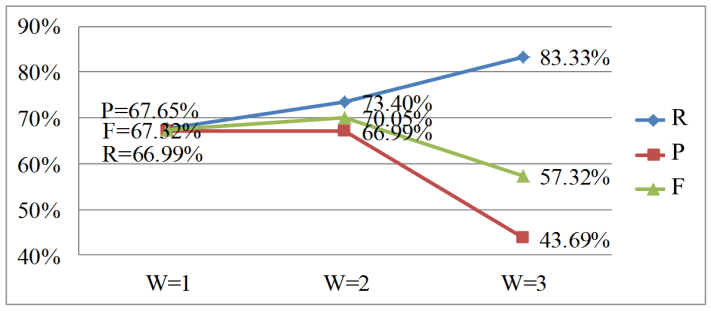
\includegraphics[height=150pt]{3-2.png}
\caption{Hotel语料评测结果}
\label{fig3-2}
\end{figure}

\begin{figure}[htp]
\centering
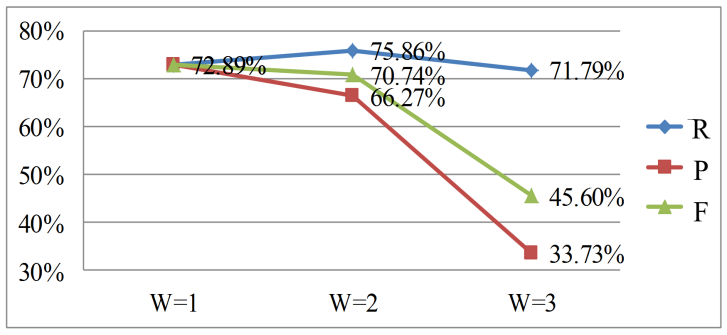
\includegraphics[height=150pt]{3-3.png}
\caption{Book语料评测结果}
\label{fig3-3}
\end{figure}

\begin{figure}[htp]
\centering
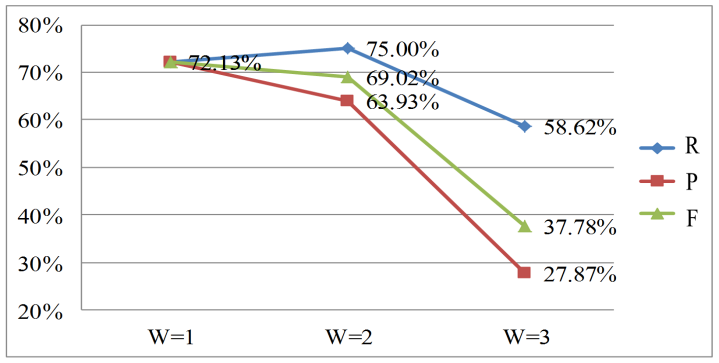
\includegraphics[height=170pt]{3-4.png}
\caption{NoteBook语料评测结果}
\label{fig3-4}
\end{figure}

当窗口$W=2$时在三个领域扩展得到的情感词数统计如表~\ref{tab3-2-3}所示。
\begin{table}[htp]
\centering
\caption{情感词典扩展统计}
\label{tab3-2-3}
\begin{tabular}{|l|l|l|l|l|l|l|l|l|l|}
\hline
\multicolumn{1}{|c|}{\multirow{2}{*}{领域}} & \multicolumn{3}{c|}{积极极性} & \multicolumn{3}{c|}{消极极性} & \multicolumn{3}{c|}{总体统计} \\ \cline{2-10} 
\multicolumn{1}{|c|}{} & \multicolumn{1}{c|}{基准} & \multicolumn{1}{c|}{扩展} & \multicolumn{1}{c|}{正确} & \multicolumn{1}{c|}{基准} & \multicolumn{1}{c|}{扩展} & \multicolumn{1}{c|}{正确} & \multicolumn{1}{c|}{基准} & \multicolumn{1}{c|}{扩展} & \multicolumn{1}{c|}{正确} \\ \hline
Hotel & 103 & 98 & 64 & 98 & 86 & 71 & 201 & 184 & 135 \\ \hline
Book & 166 & 128 & 115 & 245 & 231 & 157 & 411 & 359 & 272 \\ \hline
NoteBook & 61 & 50 & 42 & 66 & 58 & 39 & 127 & 108 & 81 \\ \hline
\end{tabular}
\end{table}

\section{基于混合方法情感词典扩展}
对基于词性特征向量的情感词典扩展方法的实验结果分析发现,在统计词语的上下文词性特征向量时,有些词在SentiHowNet中没有发现与之词性特征向量相同的情感词,无法采用基于词性特征向量方法计算情感极性值,这种情况下可以考虑采用基于连词的方法进行计算。同样的,对基于连词的情感词典扩展方法实验结果分析发现,在语料中有些情感词出现的所有句子中没有任何并列、递进或者转折连词出现,无法采用基于连词方法计算情感极性值,这种情况下可以考虑采用基于词语上下文的词性特征向量方法进行计算。两种方法可以相互补充,因此本节提出将两中方法混合使用的方法,并实验验证混合方法的性能。

\subsection{基于混合特征的情感词极性计算}
对任一选取的情感词$ w $,语集合分别采用两种方法进行极性计算,在将两种方法计算的极性值合成时,遵循以下原则:
\begin{enumerate}
\item 优先采用基于词性特征向量的方法计算出的情感极性值作为待标注词语的情感极性值。
\item 当采用基于词性特征向量的方法进行计算时,优先设置上下文窗口大小为2,其次为1。
\item 当采用基于词性特征向量的方法无法对待标注词语进行情感值计算时,采用基于连词的方法进行计算。
\end{enumerate}

具体的混合情感词语极性计算如算法~\ref{alg3-3}。
\begin{algorithm}[htp]
\caption{基于混合特征的极性计算}
\label{alg3-3}
\begin{algorithmic}[1]
\REQUIRE ~~\\
待标注词语集$\{w_1\}$;\\
极性已知词语集合$\{w_2\}$;\\
连词集合$\{c\}$;\\
每个词特征向量集合$\{V(w)|w \in \{w_1\}\cup \{w_2\} \}$;

\FOR{每一待标注词语 $w_1 \in \{w_1\}$}
\STATE 依据算法~\ref{alg3-2}计算情感极性值
\IF{$
\begin{cases}
PosScore(w_1)=0\\
NegScore(w_1)=0
\end{cases}$}
\STATE 依据算法~\ref{alg3-1}计算情感极性值
\ENDIF
\STATE 根据情感值 $PosScore(w_1)$ 与$ NegScore(w_1) $判断极性;
\STATE 将$ w_1 $加入到集合$ \{w_2\} $;
\ENDFOR
\end{algorithmic}
\end{algorithm}

\subsection{实验}
基于混合方法评测实验使用的数据、基准与评测指标与基于连词的方法~\ref{linkage}节相同。
在三个领域扩展得到的情感词数统计如表~\ref{tab3-3}所示。与表~\ref{tab3-2-3}以及表~\ref{tab3-2}进行对比,可以看出基于混合方法在每个领域的正确标注词书目数目比基于连词和基于词性特征向量的方法都有明显增加。
\begin{table}[htp]
\centering
\caption{情感词典扩展统计}
\label{tab3-3}
\begin{tabular}{|l|l|l|l|l|l|l|l|l|l|}
\hline
\multicolumn{1}{|c|}{\multirow{2}{*}{领域}} & \multicolumn{3}{c|}{积极极性} & \multicolumn{3}{c|}{消极极性} & \multicolumn{3}{c|}{总体统计} \\ \cline{2-10} 
\multicolumn{1}{|c|}{} & \multicolumn{1}{c|}{基准} & \multicolumn{1}{c|}{扩展} & \multicolumn{1}{c|}{正确} & \multicolumn{1}{c|}{基准} & \multicolumn{1}{c|}{扩展} & \multicolumn{1}{c|}{正确} & \multicolumn{1}{c|}{基准} & \multicolumn{1}{c|}{扩展} & \multicolumn{1}{c|}{正确} \\ \hline
Hotel & 103 & 103 & 64 & 98 & 100 & 88 & 201 & 203 & 152 \\ \hline
Book & 166 & 175 & 125 & 245 & 236 & 192 & 411 & 411 & 317 \\ \hline
NoteBook & 61 & 66 & 48 & 66 & 61 & 52 & 127 & 127 & 100 \\ \hline
\end{tabular}
\end{table}

对三个领域(Hotel、Book、NoteBook)的情感词典扩展实验精确率、召回率以及F值的微平均及宏平均结果如表~\ref{tab3-4}所示。表中可以看出,基于混合方法在三个领域的性能指标都比较稳定,宏平均的精确率、召回率以及F值都在74\%以上,电子产品领域性能最好(三个指标都达到78.69\%),酒店领域稍低,数据领域居中。
\begin{table}[htp]
\centering
\caption{各个领域性能评测结果}
\label{tab3-4}
\begin{tabular}{|l|l|l|l|l|l|l|l|l|l|}
\hline
\multicolumn{1}{|c|}{\multirow{2}{*}{领域}} & \multicolumn{3}{c|}{积极极性} & \multicolumn{3}{c|}{消极极性} & \multicolumn{3}{c|}{宏平均} \\ \cline{2-10} 
\multicolumn{1}{|c|}{} & \multicolumn{1}{c|}{P} & \multicolumn{1}{c|}{R} & \multicolumn{1}{c|}{F} & \multicolumn{1}{c|}{P} & \multicolumn{1}{c|}{R} & \multicolumn{1}{c|}{F} & \multicolumn{1}{c|}{P} & \multicolumn{1}{c|}{R} & \multicolumn{1}{c|}{F} \\ \hline
Hotel & 0.6214 & 0.6214 & 0.6214 & 0.8980 & 0.8800 & 0.8889 & 0.7549 & 0.7476 & 0.7512 \\ \hline
Book & 0.7837 & 0.8136 & 0.7983 & 0.7530 & 0.7143 & 0.7331 & 0.7711 & 0.7711 & 0.7711 \\ \hline
NoteBook & 0.7869 & 0.7273 & 0.7559 & 0.7879 & 0.8525 & 0.8189 & 0.7869 & 0.7869 & 0.7869 \\ \hline
\end{tabular}
\end{table}

为了综合比较本章的三种方法,基于连词的情感词典扩展、基于词性特征向量的情感词典扩展和混合方法的情感词典扩展的实验评测宏平均结果对比情况如图~\ref{fig3-5}、图6~\ref{fig3-6}和图~\ref{fig3-7}所示,从比较结果来看,混合方法在性能是在三个领域语料中均是最优的,是比较理想的情感词典扩展方法,其次为基于词性特征向量的方法(取窗口为2时),基于连词方法性能接近于词性特征向量的方法。因此在选择对SentiHowNet情感词典扩展方法时,优先选择混合方法。

\begin{figure}[htp]
\centering
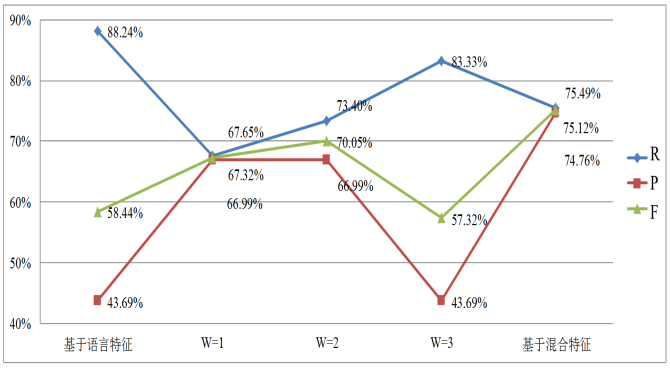
\includegraphics[height=200pt]{3-5.png}
\caption{Hotel语料评测结果综合比较}
\label{fig3-5}
\end{figure}

\begin{figure}[htp]
\centering
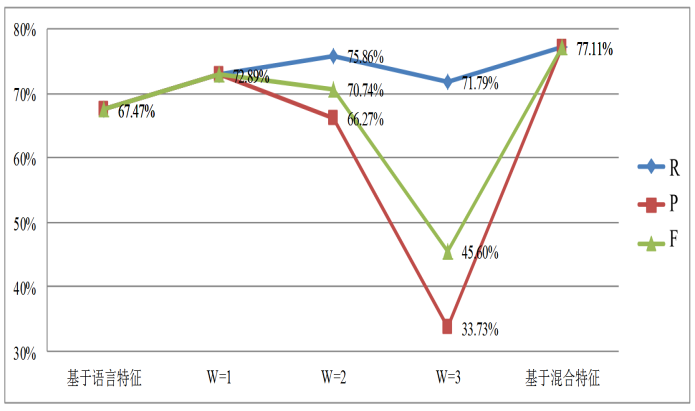
\includegraphics[height=200pt]{3-6.png}
\caption{Book语料评测结果综合比较}
\label{fig3-6}
\end{figure}

\begin{figure}[htp]
\centering
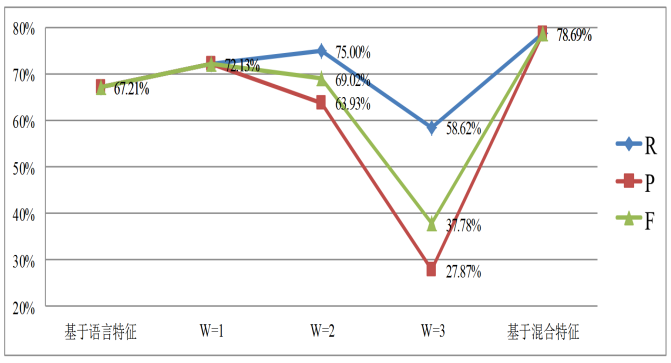
\includegraphics[height=200pt]{3-7.png}
\caption{NoteBook语料评测结果综合比较}
\label{fig3-7}
\end{figure}

\section{小结}
本章详细讨论了基于语料资源的中文情感词典的三种扩展方法,并用三个领域的语料进行了实验验证。第一种方法是基于连词语言线索方法,该方法根据语言中连词对词语语义倾向的限制作用,选择了并列、转折以及递进三类连词来进行词典扩展,设计了基于连词的情感词的极性值计算方法以及详细算法,实验验证了中文连词在情感词典扩展中的有效作用;第二种方法是基于词性特征向量的方法,根据出现在相同上下文的词语语义相似性,设计词语的词性特征向量,统计具有相同词性特征向量的情感词进行情感极性值计算,并设计了详细算法,实验结果证明了词性特征向量的有效性;第三种方法为一二种方法的混合,可以起到相互补充的作用提高情感词的识别准确性,实验结果证明混合方法在三种方法中在三个领域中最为稳定,达到最好性能。


\chapter{无监督的自举式情感分类}
\label{ch4}

\section{引言}
\label{ch4_intr}
文本的情感分析是挖掘文本中主观性信息学的主要手段,是研究文本中观点、态度、情绪和立场等主观性信息是如何表达的。情感分析技术可以从数量庞大的文本数据中抽取并总结主观性信息,为后续的一些应用(商业智能(Business Intelligence),舆情分析(Public Opinion Analysis)或选举预测(Election Prediction)等)提供技术和工具支持\upcite{Liu2012}。在社交媒体中,一些基于文本的平台比如微博产生了大量针对各种话题或实体的带有主观性信息的数据。这对这些数据的分析,也就是情感分析正逐渐受到各个研究领域(比如推荐系统和搜索引擎)的重视。情感分析中一个主要的方法就是应用各种分类技术,也就是根据作者的主观态度将文本进行分类,一般将这种研究称为情感分类研究。情感分类一般是从一些标注过的训练数据中通过学习得到一个分类模型,学习得到能够将一种情感类型区别于其他类型的一些特征\upcite{LourencoJr2014}。这种模型的性能主要依赖于其能够学习到的数据中出现的情感的文本表达模式,一般是文本中出现的词语、短语或者词语的各种组合。情感分类也就是情感分析的分类形式,虽然可以被视作文本分类的特殊形式,实际上情感分类是比文本分类更具挑战的任务,因为文本中情感的表达方式严重依赖领域和上下文环境\upcite{jiang2011target,}。

随着微博(Twitter、新浪微博等)的出现和广泛使用,用户产生内容(UGC,User-Generated Content)成指数增长,这些内容并且这些内容对于我们来说是很容易获取的,并且这些内容里面有很多用户对于各种话题的观点和情感等主观性信息。因此我们可以很方便的从这些数据中提取出主观性信息,并使其在商业、旅游或者健康领域得到应用。但是对微博进行情感分类特别具有挑战性,因为(1)用户使用微博表达观点的方式是多种多样的,既有正规传统语言的表达方式,又有社交媒体特有的流行的表达方式,比如"coooooool", “OMG",":-(",“屌丝”,“逆袭”等,这些表达方式虽然对于人来说是比较直观和易于理解的,并且更加方便了用户的在线交流,但是对于计算机来说,却是很难准确确定这些表达方式的观点和情感等语义信息。(2)更具挑战性的是,因为用户群体的复杂性,经常会有用户创造出的一些缩写词或者新词,并且会将一些传统的词赋予新的语义在微博中重新使用,这些语言上的变化使得微博上观点的表达方式有别于传统文本的表达方式。综上所述,可以看出微博中的文本噪声、非正式本质以及语言词汇的急剧膨胀使得对微博中表达的主观性信息自动分析需要依赖于微博这种独特的语言环境,因此进行情感分类是困难的。这种情况被称为微博情感分类的领域(或语言环境)依赖问题,也就是使用其他文本数据集(比如评论或博客)训练出的分类器在微博的情感分类时会出现性能急剧下降,而要获得大量微博训练数据集需要大量的人力,并且微博数据具有时效性,不同时间阶段的微博数据集中观点表达方式也会产生漂移。

本章我们主要关注微博情感分类的领域依赖性问题。为了解决这个问题,基于我们的一些观察,我们提出了一种无监督的自举式(bootstrapping)情感分类框架。该框架首先使用现有的已经有情感标签的语言资源训练得到一个通用的能够跨领域使用的分类器;然后再根据该分类器的跨领域特点使用其作为初始分类器对微博进行分类,获得一些高可信度的微博作为训练集训练得到一个微博分类器;将两个分类器结合迭代使用共同训练(Co-training)过程,逐步在目标数据集扩展并训练微博分类器,直至其分类性能达到最优。

\section{相关工作}
\label{ch4_relt}
情感分类在观点挖掘研究中越来越受到重视,前期工作主要研究针对评论(商品或电影)进行情感分类。经常使用的方法可以分为基于规则的方法和基于学习的方法,其中基于机器学习方法性能一般比较好因而常被用来作为对表的标准\upcite{Pang2002}。

现在研究人员逐渐开始注意到微博中用户的主观性信息,并开始结合微博的语言特点进行对微博进行情感分类研究。一些研究显示可以将微博的一些独特的特征结合进情感分类方法中。比如,Barbosa和Feng~\upcite{Barbosa2010}提出了两阶段支持向量机分类器(Support Vector Machine (SVM) classifier)对tweet进行情感分类,证明了该分类其能对tweet的类别偏置(biased)和噪声具有很好的鲁棒性;Hu等~\upcite{Hu2013}将社交媒体数据中的情感表达解成情感指征(emotion indication)和情感关联(emotion correlation)两种信号,通过对两类情感信息进行联合建模方式实现了对微博的无监督情感分类;Jiang等~\upcite{jiang2011target}主要关注依赖于特定目标的微博情感分类,提出了通过将目标依赖特征(target-dependent features)和相关微博同时进行考虑的监督学习方法,并证明了可以提升情感分类性能;Wang等~\upcite{wang2011topic}针对hashtag级别的情感分类进行了研究,并提出了一个全新的图模型,然后使用提升(boosting)式分类方法进一步提高了模型的性能;Amir等~\upcite{AsiaeeT2012}针对单条微博的情感分类提出了一个分层分类器框架,框架通过抽取对特定目标的微博,将微博按情感类型分开以及分离正负情感类型微博三个层次进行有监督的分类学习;Hu等~\upcite{hu2013exploiting}基于社交理论抽取微博之间的情感关系,提出了一种全新的社会学方法使用这些情感关系以促进情感分类性能,并有效解决了数据中的噪声问题;同样受到社会学理论的启发,Guerra等~\upcite{CalaisGuerra2011}依据人类通常会持有一致的带有偏执的观点,提出了全新的迁移学习(transfer learning)方法解决微博基于话题的实时情感分类问题;Thelwall等~\upcite{Thelwall2010,Thelwall2012}设计了SentiStrength情感分析工具,用于对微博等社交媒体中非正式语言中的情感分析,该工具是基于规则的方法,使用了人工编辑的词典并结合了微博语言中的句法和拼写特点抽取微博中的情感强度,该工具获得了广泛的应用。

以上这些工作通过利用微博的一些网络和语言特点对情感分类方法进行了适应性的改进,以使得这些方法能够适用于微博语言环境,但是没有彻底解决微博情感分类问题的语言环境依赖问题,本章我们提出的方法从一个全新的视角来看情感分类问题,将情感分类的特征空间分各位环境依赖部分(context-dependent part)和环境独立部分(context-independent part)分别进行训练分类器,然后将两种分类器结合进一个自举式(bootstrapping)学习框架中。

\section{问题的形式化}
\label{ch4_form}
简单来说,情感分类主要目标就是将文本分类为预先定义的情感极性类别(一般是积极的,positive或消极的,negative)。形式化上,对于给定的文档语料库$ D=\lbrace d_{1},\dots ,d_{n} \rbrace$,预定义的情感类别$ Y=\lbrace 1,-1\mid \mathrm{positive}=1,\mathrm{negative}=-1 \rbrace$,情感分类的任务就是对每一个文档$ d_{i} $预测一个类别标签$ y_{i} $。为了与文本分类问题一致,每个文档可以表示为一个特征向量$ x=R^{n} $,$ n $表示特征空间的大小对于情感分类问题来说,对于每一个特征通常将其权重定为二值的,1表示特征在文档中出现,0表示没有出现\upcite{Pang2002}。对于有监督的机器学习,给定训练集$ D=\lbrace x_{1},\dots,x_{m} \rbrace $,可以学习到分类器:
\begin{equation}
\label{e1}
  f:D \longrightarrow Y, Y=\lbrace 1,-1 \rbrace \enspace .
\end{equation} 
对于未来文档$ x $,同样将其表示为特征向量$ x=\left( w_{1},\dots,w_{v} \right)  $($ w_{i} $表示第$ i $维权重),就可以使用该分类器去预测其情感类别:$ f \left( x \right)   $。

在以往的情感分类研究中,有一个潜在的假设,就是用于表示文本的特征向量中所有的特征(一般是词语)在表达情感极性时作用是相同的,也就是其出现与否可以在所有的文本中表达相同的情感。实际上这种假设是不成了立的,因为有些词语表达的是客观信息,有些表达主观信息,而且即便是表达主观信息,作用也都不一样。因为有些词语无论用在那种领域或语境下都能表达同样的情感,而有些词语只能在某些具体的语境下表达某种情感。以下面这条微博为例:

\begin{description}
\item{tweeet:} @Kid\_Cloudz: Happy birthday to Yessicaaaa! :D lovee you feggit wish you the best day everrrrr!!!!! @030268.
\end{description}

以词袋模型(bag-of-words)为例,所有的词语都应该抽取出来作为特征加入到特征向量中同等地用于对这条微博的情感倾向进行建模。然而,仔细观察就会发现,微博中有些词语(@Kid\_Cloudz, :D, lovee, everrrrr,!!!!!)实际上只能在微博这种语境中出现并且表达出某种情感倾向,而另外一些词语(Happy, birthday, wish, best, thanks)无论在什么领域或语境下都是正面情感倾向的的标识。基于这样的直观认识,我们可以提出以下特征空间划分的假设:

\begin{theorem}[假设]
\textbf{特征空间划分假设:} 对于微博情感分类问题的特征向量空间,可以将其所有的特征划分为以下两个部分:
\begin{itemize}
\item{领域独立部分:}也就是通用的特征,该部分特征在任何领域和语言环境下都是某种情感倾向的表达方式。
\item{领域依赖部分:}也就是具体语言特征,这部分特征只有在微博这种语言环境下才能有具体的语义和表达一定的情感倾向。
\end{itemize}
\end{theorem}
这个假设可以更加形式化的表示,对于情感分类问题中一条微博的特征向量$ x=\left(  w_{1},\dots,w_{l},w_{l+1},\dots,w_{v} \right) $,可以划分为两个部分:

\begin{equation}
\label{e2}
x=\left\{
\begin{array}{rcl}
x_{g}     & \qquad        &:\mbox{general features}\\
x_{c}     &  \qquad       &:\mbox{context features}
\end{array}
\right. \enspace .
\end{equation}
其中,$ x_{g}= \left( w_{1},\dots,w_{l}\right) $是特征向量空间的通用部分,而$ x_{c}= \left( w_{l+1},\dots,w_{v}\right) $是领域依赖部分。

基于以上假设,情感分类问题可以进一步形式化定义为:

\begin{definition}[情感分类]
根据假设(1),情感分类问题可以表示为$(X_{g},X_{c},Y)$,其中:
\begin{itemize}
\item $ X_{g}\subset R^d$和$ X_{c}\subset R^p$为两个输入特征空间,$d+p=n$,分别表示两部分空间的维度;
\item $Y$为输出空间,一般表示为二值空间$ Y=\lbrace 1,-1\mid \mathrm{positive}=1,\mathrm{negative}=-1 \rbrace$;
\item 假设有一独立同分布(independently identically distributed)微博实例集合$D=\{(x_i^g,x_i^c,y_i);i=1\ddots m\}$,该集合是从空间$P=X_g \times X_c \times Y$中采样得到,向量$x_i^g$表示实例领域独立部分特征,向量$x_i^c$表示领域依赖部分特征,$y$表示实例微博的情感类别;
\end{itemize}
实际上经过特征空间的划分提供了对于同一微博的两种不同的视角(view),因此可以将数据集$D$看作是$D_g=\{(x_i^g,y_i);i=1\ddots m\} \in (X_g \times Y)^m$和$D_c=\{(x_i^c,y_i);i=1\ddots m\} \in (X_c \times Y)^m$两种不同的集合,因此对于集合$D$的情感分类问题可以视为构建两个分类器通用情感分类器(General Sentiment Classifier)和微博情感分类器(Context Sentiment Classifier):
\begin{equation}
\begin{cases}
General Sentiment Classifier:f_g:X_g \mapsto Y\\
Context Sentiment Classifier:f_c:X_C \mapsto Y
\end{cases}
\end{equation}
\end{definition}
当然基于部分特征空间的分类器性能上是否会降低还是一个值得研究的问题,但是本章我们主要研究以下几个问题:
\begin{enumerate}
\item 对于从实例中抽取到的同一个特征空间,怎么确定特征空间中领域依赖和领域独立两部分特征?
\item 得到不同的特征空间后,使用什么样的训练数据集来训练得到两个不同的分类器?
\item 两种独立的分类器比同一空间分类器性能上会有什么样的变化,如何将两种分类器结合起来达到更好的性能?
\end{enumerate}

\section{无监督的情感分类框架}
\label{ch4_frame}
在微博语言中,除了正规的表达方式方式外,一些语言因为比较难以理解而常被视为“火星文”,尤其是对于不长使用微博的人来说对于一条微博中出现的一词语可能不理解其语义。但是整条微博的情感倾向性确能够比较容易读懂,因为微博常常是正规表达方式和“火星文”混合在一起使用的,理解了正规表达部分,也就能理解了整条微博的情感倾向。直观上,这种现象可以通过我们的特征空间分割假设来解释,正规表达部分特征也能从一个不同的视角(view)来阐释整条微博的主观情感。而这些正规表达部分特征$ x_{g} $是不以来于微博语境的,对于任何人(长使用微博的或是很少使用微博的)都是易于理解的。

相似的,对于微博的自动情感分类,基于我们特征空间分割假设,可以认为一条微博的情感倾向性可以通过两部分特征都识别出来。也就是说,如果能够对与一些通用的情感表达知识,在某种程度上也能识别出一条微博的情感极性(根据微博中正规表达方式的比例不同,比例越大就越容易识别)。实际上有很多研究者已经开始研究如何建立各种情感词汇表来对这种通用的情感知识进行建模了,比如我们前面章节的工作中提到的OpinionFinder词典\upcite{Wilson2005,Wilson2009}、ANEW词典\upcite{Bradley1999}、AFINN词典\upcite{Nielsen2011}、SentiWordnet\upcite{Esuli2006}、HowNet情感词典\upcite{2013},NTUSD情感词典\upcite{Ku2007}、情感词汇本体词库\upcite{2013a}以及我们的SentiHowNet\upcite{谢松县2014}。虽然这些词典在尝试着建立通用的情感表达知识库,但是由于存在一词多义现象,使得一个词语的具体情感倾向性还是需要具体的语言上下文进行“消歧”。因此能够真正找到通用的资源来对跨领域情感知识进行建模不是一件容易的事。但是这样的知识资源却是存在的,比如成语和谚语等具有明确无歧义的情感倾向性,如何能够利用这样的知识资源对通用情感知识进行建模是本章研究的重点。

\subsection{通用情感分类器}
\label{general}
在语言资源中有许多对情感分类研究非常有用的资源,其中成语资源就是其中之一。成语(或谚语,本章中用成语通指这两种语言资源)无论在中文还是英文中都存在,比如中文的“空中楼阁”、英文的``bring down the house''(搏得满堂喝彩)等。这些成语的情感倾向性是固定不变的,不会随着领域或语境的不同而有歧义。这与我们的通用情感分类器需求十分契合,实际上有很多的专门针对成语编辑的词典资源,为通用情感分类器提供了很好的数据集进行训练。一般的成语词典的条目如下所示:
\begin{description}
\item{空中楼阁:}贬义词,形容虚构的事物或不现实的理论、方案,脱离实际的理论、计划及空想。
\end{description}
在“空中楼阁:”条目中,有三部分组成:成语本身、情感倾向性(贬义,属消极情感)以及该成语的释义部分。其中释义部分有几个同
There are many linguistic resources highly valuable for sentiment classification, of which idiom resources attract interests of this research. 
Idioms are common phenomena of many languages beside Chinese, such as ``castles in the air'', ``a bed of thorns'', and ``bring down the house'' in English.
As is convinced, the sentimental polarity of idioms is independent and unchangeable under any context. 
There are many off-the-shelf idiom lexicons in all kinds of languages with entries taking the example form as:

\textit{castles in the air: a derogatory term, indicate the illusive things or impractical fanciness metaphorically.}

In this example, the entry is composed of three parts: the idiom ``castles in the air'', the semantic orientation ``a derogatory term'' representing negative
sentimental polarity and a short paraphrase with three general negative words (``illusive, impractical and fanciness''). 
The example provides us with a labelled sentimental instance with general sentiment features and a negative label.
Most importantly, the sentimental polarity of such instance is independent of any context just as the idiom it explains. 
Based on such observation, another hypothesis is proposed as follows:
\begin{hypothesis}
\label{h2}
The sentimental polarity of the idiom paraphrase is independent of language context just as the idiom it describes.
\end{hypothesis}
With Hypothesis~\ref{h2} admitted, we could constructed a training dataset with the features extracted from paraphrases of idioms as general feature vector, the sentimental polarity of idioms as sentimental labels. 
Then a context-independent classifier could be trained to model the general sentiment knowledge.

\subsection{Context Sentiment Classifier}
\label{context}

As the general sentiment features are only one part of all features in the whole feature space, the other context-dependent part of features should be considered in order to capture the subtle clues embedded in the specific sentiment expressions in language context of microblogs.

To model the context-dependent part of tweets, there are two questions must be solved. 
The first is to identify the context-dependent part of features extracted from tweets. 
In fact, new expressions appears on microblogs with the explosively increasing of UGC, which makes it rather difficult to clearly tell whether each word is context dependent or not. 
However tweets are conventionally short with the limitation of 140 characters, and users often express one particular sentiment in one tweet with a few words. 
Based on the particular characteristics of tweets, we make an assumption that if a tweet contains idioms,  sentimental polarity of words in a tweet are often context-dependent except for the idioms. 
The second is how to find labelled instances to train the context-dependent classifier. 
Some researchers have proposed distant supervision to solve the training data shortage of Twitter \cite{xsongx:b36,xsongx:b37}. 
In this paper we establish our training dataset in a similar way.
We retrieve tweets on microblogs and try to get as many tweets as possible that contains idioms. 
By stripping off idioms, we extracted context-dependent features from left words, and took the sentimental polarity of idioms as labels. 
So we get our noisy labelled dataset and a context-dependent classifier is trained to model the context-dependent knowledge.

\subsection{Combination of Two Classifiers}
\label{combination}

Although theoretically the general classifier and context classifier could be able to model different sentiment knowledge separately and classify the sentiment of a tweet accurately to some extent, the coverage and efficiency of them are limited by the quality and quantity of training datasets. 
Besides, it is obvious that the paraphrase of idiom and tweet segments (lefts by stripping off idioms) is usually very short, so the feature vectors of datasets must be very sparse, which degrades the performance of the classifiers. 
For above reasons, a consistent bootstrapping machine learning framework is chosen to combine the two classifiers together. 
The framework is illustrated in Figure~\ref{fig1}. 
\begin{figure*}[!t] 
\centering%
\includegraphics[width=6.0in,height=2.8in]{itse13p.pdf}
\caption{The Bootstrapping Sentiment classification Framework}
\label{fig1}
\end{figure*}
As illustrated in the framework, in an iterating manner, the general classifier $ P_{g} $ and context classifier $ P_{c} $ are applied to test dataset so that the every test instance $ x_{i} $ is predicted labels $ c_{i}=\lbrace c_{g},c_{c}\rbrace $ initially, with confidence $ p_{i}= \lbrace p_{g},p_{c}\rbrace$. 
Then a combined confidence score is calculated with Equation~\ref{e3}:
\begin{equation}
\label{e3}
p_{i}=\left\{
\begin{array}{rcl}
\lambda\ast p_{g} + \left( 1-\lambda \right) \ast p_{c} \qquad \mbox{if} \quad c_{g}=c_{c};\\
0 \qquad \mbox{if} \quad c_{g} \neq c_{c};
\end{array}
\right. \enspace .
\end{equation}
where $ \lambda $ is the coefficient to control impacting weights of different part of features. 
We initialize $ \lambda = 0.5 $ with equal weights of general part and context part of features, and to make combined classifier more adaptable for microblogs, we  increase the weight of context part step by step with the bootstrapping iteration progressing.
The test dataset initially labelled as $ c_{i} \left( c_{i} \in \lbrace 1, -1\rbrace \right)$ was sorted with descending confidence $ p_{i} \left( p_{i} \neq 0 \right) $ for two sentimental categories $ C=\lbrace 1,-1\rbrace $ separately.
The $ n $  positive and negative instances with top high confidence are selected as new instances to add into the training dataset and improve the context classifier to a more context-aware classifier. 
Such a procedure iterates until convergence.
The output of such semi-supervised sentiment classification framework is the predicted results of test dataset. 
Above all, the whole framework can combine the two classifiers which constructed on divided feature space into a stronger classifier. 

\subsection{Classifier Description}
\label{classifier}

We adopt the same methods as Pang et al.~\cite{xsongx:b4}, in that they have applied Na\"\i ve Bayes, Maximum Entropy and Support Vector Machine classifiers to identify the effectiveness of machine learning techniques on sentiment classification, and they got satisfying result (accuracy of 82.9\%).
\subsubsection{Na\"\i ve Bayes Classifier.}
\label{bayes}
Naïve Bayesian classifier is the most popular text classification techniques.
For sentiment classification problem as formulated in Section~\ref{formulation}, to determine which sentimental category $ c_{j} $ a document $ d_{i} $ belongs to, it is needed to compute the posterior probability $ P \left(c_{j} \mid d_{i} \right)$. 
According to the Bayesian probability and the multinomial model, based on the hypothesis that the probabilities of features $ w_{d_{i},k} $ are independent given document class, Equation~\ref{e4} is got:
\begin{equation}
\label{e4}
P \left(c_{j} \mid d_{i} \right) = \frac{P \left( c_{j} \right)\prod_{k=1}^{| d_{i} |} P \left( w_{d_{i},k} \mid c_{j} \right)}{\sum_{r=1}^{|C|}P \left( c_{r} \right)\prod_{k=1}^{| d_{i} |} P \left( w_{d_{i},k} \mid c_{r} \right)} \enspace .
\end{equation}
The class with the highest probability is assigned as the sentimental category of the document $ d_{i} $. 
\subsubsection{Maximum Entropy Classifier.}
\label{entropy}
The Maximum Entropy classifier assigns the class with the higher conditional probability to the sentimental category of document $ d_{i} $ as follows:
\begin{equation}
\label{e5}
P \left( c_{j} \mid d_{i}, \overrightarrow{\theta} \right) = \frac{1}{Z}exp \left( \overrightarrow{\theta}, \overrightarrow{f} \left( d_{i},c_{j} \right) \right) \enspace .
\end{equation}
where $ \overrightarrow{\theta} $ denotes the vector of feature weights, $ \overrightarrow{f} \left( d_{i}, c_{j} \right)$ denotes feature function that maps pair $ \left( d_{i}, c_{j} \right) $ to a feature vector, and $ Z $ denotes normalization factor.
With labelled dataset $ D $, the training procedure is trying to solve such an optimization problem as:
\begin{equation}
\label{e6}
\overrightarrow{\theta^{\ast}}=argmax_{\overrightarrow{\theta}}\prod_{i=1}^{|D|} P \left( c_{j} \mid d_{i}, \overrightarrow{\theta} \right) \enspace .
\end{equation} 
\subsubsection{Support Vector Machine Classifier.}
\label{svm}
Support Vector Machines classifier (SVM), is a kind of discriminative method of machine learning techniques.
SVM tries to find a decision surface to separate the training data into two classes and makes decisions based on support vectors. 
In this research, linear SVM has been adopted due to its popularity and sound performance in sentiment classification task.
The training of SVM is trying to minimize an constraint optimization problem:
\begin{equation}
\label{e7}
\begin{aligned}
\overrightarrow{\alpha^{\ast}}=argmin \left( -\sum_{i=1}^{n}\alpha_{i} + \sum_{i=1}^{n} \sum_{j=1}^{n}\alpha_{i}\alpha{j} x_{i}x_{j}<\overrightarrow{x_{i}},\overrightarrow{x_{j}}> \right)\\
\mbox{Subject to:} \sum_{i=1}^{n}\alpha_{i}y_{i}=0 , 0\leqslant \alpha_{i} \leqslant 1
\end{aligned} \enspace .
\end{equation}

\section{Experiment}
\label{experiment}

In this section, the proposed semi-supervised sentiment classification framework is verified in an empirical test. 
The test has been carried out with Chinese dataset constructed from an off-the-shelf on-line idiom dictionary and microblog platform Tencent\footnote{\url{http://t.qq.com/}}. 

\subsection{Experiment Description}
\label{description}

\paragraph{Dataset}
We crawled the on-line idiom dictionary from China Education Network\footnote{\url{http://chengyu.teachercn.com}} and got an idiom dataset of 8,160 instances labelled with positive (3,648 instances) and negative (4,512 instances) sentiment, which was used to train the general classifier. 
From Apr.15th,2013 to May 1st,2013, we monitored Tencent time-line tweet streams, retrieved and extracted the tweets that contained at least one idiom in our idiom dataset, resulting in about 120,346 tweets. 
After stripping off idioms from all tweets and removing tweets with characters less than 4, we got a dataset of 91,268 instances which was used to train context classifier. 
The dataset from the First Chinese tweet Sentiment Analysis and Semantic Relationship Extraction Evaluation of CCF Natural Language Processing and Chinese Computing\footnote{\url{http://tcci.ccf.org.cn/conference/2012/pages/page04_eva.html}} was used to evaluate performance of our framework. 
\paragraph{Classifiers and performance measurement}
There are various complicated measurements to evaluate the performance of computational algorithm, of which the simplest accuracy index was chosen to evaluate the performance of our framework, because the comparison between measurements was not the important points of our research. 
As for classifiers, Na\"\i ve Bayes classifier and Maximum Entropy classifier of NLTK (Natural Language ToolKits) \cite{xsongx:b27} package and Support Vector Machine classifier of Libsvm \cite{xsongx:b28} package were used for classification. 
All the parameters and settings were optimized by cross-validation.
\paragraph{Baseline and upper bound}
Two baselines were used to compare with the proposed framework, the first one was na\"\i ve $ 50\% $ baseline since the test dataset was balanced with respect to the sentiment classes, the other one was the traditional lexicon-based classifier by comparing the number of positive words and negative words in HowNet sentiment lexicon for a tweet to determine its sentiment class.
As mentioned in Section~\ref{related}, supervised machine learning methods are often used as upper bound to be compared by other methods. 
In the experiments, an upper bound was also set up with test dataset in the five-folded cross-validation manner.
\paragraph{Preprocessing}
Text written in Chinese are not well formatted in that words in a sentence are not separated by space as English. 
All the text in Chinese must be segmented before bag-of-words features being extracted. 
In the experiment, all text of training and testing dataset were segmented with Chinese segmentation software ICTCLAS\footnote{\url{http://ictclas.nlpir.org/}}.

\subsection{Result and Analysis}
\label{result}
To determine the values of $ \lambda $ in Equation~\ref{e3}, we carried out traversal experiment by varying the value of $ \lambda $ from $ 0 $ to $ 1 $ with step of $ 0.1 $. The result is illustrated in Figure~\ref{fig2}.
\begin{figure}[!t]
\centering
\includegraphics[width=3.5in,height=2.0in]{lambda.pdf}
\caption{The Impact of $ \lambda $ on Different Classifiers: NB denotes Na\"\i ve Bayes, MX denotes Maximum Entropy and SVM denotes Support Vector Machine.}
\label{fig2}
\end{figure}
The values of $ \lambda $ for each combined bootstrapping classifier based on three different classifiers are fixed as the accuracy reaches its peak, which are: $ 0.4 $ for Na\"\i ve Bayes classifier, $ 0.5 $ for Maximum Entropy classifier, and $ 0.3 $ for Support Vector Machine classifier.

The final sentiment classification results are shown in Table~\ref{t1}. 
\begin{table}[!t]
\caption{Results for Different Classifiers}
\label{t1}
\centering
\begin{tabular}{|l||l|l|l|}
\hline
%\noalign{\bigskip}
\bfseries Classifier &  \bfseries NB    &   \bfseries MX    &   \bfseries SVM    \\
%   & Lexicon  & Supervised & General & Context &  Combined \\
%\noalign{\bigskip}
\hline
%\noalign{\bigskip}
\bfseries Lexicon Classifier & 0.725 & 0.725 & 0.725 \\
\hline
\bfseries Supervised Classifier & 0.785 & \textbf{0.806} & 0.826 \\
\hline
\bfseries General Classifier & 0.734 &  0.740 & 0.762 \\
\hline
\bfseries Context Classifier & 0.766 & 0.785 & 0.805 \\
\hline
\bfseries Combined Classifier & \textbf{0.802} & 0.802 & \textbf{0.843} \\
% NB & 0.725 & 0.785 & 0.714 & 0.766 & \textbf{0.802}   \\
% MX & 0.725 & \textbf{0.806} & 0.740 & 0.785 & 0.802  \\
% SVM & 0.725 & 0.826 & 0.722 & 0.805 & \textbf{0.843} \\
%\noalign{\bigskip}
\hline
\end{tabular}
\end{table}

Firstly, the accuracies of general classifier and context classifier all surpass the na\"\i ve baseline (50\%), which proves that they are superior to random selection and may be better choice when there are no labelled dataset available for supervised or semi-supervised machine-learning sentiment classification.

Secondly, the accuracy of general classifier is a little higher than the traditional lexicon-based classifier, in that although they can both model the general sentiment knowledge, the general classifier is trained on context-independent part of features, so it can better catch the holistic sentimental polarity of tweets, while the sentiment lexicon often contains ambiguous entries. 
As for the context classifier, the performance outperforms the traditional lexicon-based classifier and general classifier, because it has been trained on context-aware part of features, and the users are more willing to express their sentiment with ``Mars Language'' of microblogs, so the context classifier is more adaptable for microblog context.

Finally, the combined classifier shows the best performance by combining general classifier and context classifier. 
It even outperforms the upper bound supervised classifier, which proves the effectiveness our proposed framework because it can not only catch the holistic sentimental polarity of tweets by modelling general sentiment knowledge but also adapt to the microblog language context by considering the subtle sentiment expressions articulated in tweets.

\section{Conclusion}
\label{conclusion}

Context-dependent problem has always been a main challenge of sentiment classification.
In this paper, we have proposed a novel semi-supervised framework to get it solved in the microblog language context. 
From a different perspective of feature space, we put forward the assumption that feature space can be divided into the general part and the context part.
To make use of two parts of features, two classifiers are trained on dataset constructed from idiom resources and tweets separately. 
Our framework combines the classifiers with a semi-supervised bootstrapping learning algorithm. 
The experiment results show that the proposed framework could outperform the state-of-art supervised classifier. 
In future, we will try to improve the sentiment classification performance by enlarging the context-independent resources and extracting richer features besides bag-of-words feature.
\chapter{用户主观性建模}
\label{ch5}

\section{引言}
上一章介绍了如何对社交媒体中文档进行情感分类以确定文档表达的观点倾向性,本章将在上一章的基础上介绍用户层面的观点分析,主要包括如何对用户发表的多个文档中的观点信息进行集成,并以一种合理方式对集成的观点进行表示。

随着基于内容的社交媒体的兴起,越来越多的用户开始在社交媒体上针对各种话题发表短的文本信息表达意见和观点。本章研究的用户主观性是就是指用户感兴趣的话题(产品、政治人物和事件等等)以及用户对这些话题所持观点。一方面,社交媒体的文本数据因为覆盖话题广泛和用户观点信息丰富而成为研究用户主观性的重要数据来源。另外一方面,使用社交媒体数据研究用户的主观性反过来也会有利于针对社交媒体的后续研究及应用,比如用户观点查询、观点追踪或者用户行为的预测等研究,在社会学、心理学、政治以及商业领域具有重要作用。社交媒体中用户产生的内容数量巨大,而用户产生的文本信息短小分散,以碎片化形式存在于海量的社交媒体数据中,因此用户的主观性信息是散布在“碎片化的信息”中,使得从这些数据中挖掘和分析用户各种观点变得极具挑战性。例如,如果在Twitter中查询“iphone”(由于Twitter数据的实时流动性,不同时间查询会有不同的结果,此处结果查询日期为2014年2月14日),会返回大概231,233用户的830,879条微博(tweet,本文中统称为微博),意味着很多用户发表了不止一条微博来表达对“iphone”的观点。因此为了能够更好的了解到不同用户各种不同的观点,需要能够自动从用户发表的所有内容(UGC)中挖掘出“碎片化的观点”,将这些主观性信息进行集成(integrate),然后呈现出用户对于“iphone”这一感兴趣话题的整体观点\upcite{Lu2008}。实际上用户感兴趣的话题会有很多,发表的信息也是多种多样的,因此如何从一条条独立的“信息碎片”中找到用户感兴趣的话题和观点对用户主观性研究来说是很有意义的。

本章针对用户观点信息集成建模问题提出了主观性模型概念,在一个框架将话题和观点结合起来。主观模型分为两部分,一部分是用户感兴趣话题分布,用于用户对各种话题的兴趣度建模;另一部分是用户在每个话题上的观点分布,用于用户对话题发表的多个观点信息集成建模。图~\ref{fig5-1-1}展示了主观模型框架的总体结构,具体来讲,该框架通过三个步骤来解决用户话题观点集成问题:(1)首先使用用户层次的话题模型(user-level topic model)从用户发表的微博(以Twitter平台为例,当然该框架也可以适用于其他社交媒体平台)中抽取出用户感兴趣的话题;(2)使用话题模型和情感分析技术对用户每条微博进行话题和观点分析;(3)综合并集成用户所有微博的话题与观点信息形成用户的主观模型。

本章具体安排为:首先介绍相关工作,然后定义了用户层面的观点集成问题,接着给出主观模型定义以及构建方法,并以观点预测实际应用为例对主观模型进行了定性定量实验评测,最后是小节。

\section{相关工作}
\label{ch5_sec2}
虽然观点挖掘(Opinion mining)研究最先是在商品评论(Review)和新闻评论(Comment)\upcite{Pang2008OMS,Liu2012}领域兴起的,近年来越来越多的工作开始关注于Twitter等社交媒体短文本的观点信息,目前工作重点主要是针对单个短文本进行情感分析\upcite{Barbosa2010,Davidov2010,Jiang2011,Li2010,tan2011user},往往忽视了社交媒体的文本信息不是独立的,用户之间、数据之间以及用户与数据之间存在广泛联系。还有一些工作开始着眼于研究用户层面(User level)的主观性信息\upcite{Mostafa2013,Malouf2008},研究还主要是识别用户发表观点针对的目标\upcite{Liu2010}或是针对特定目标分析用户的观点倾向性\upcite{Zhai2011},而没有考虑到用户关心的多个话题、话题的各个方面(aspect)以及各方面观点的集成。自从Blei等\upcite{Blei2003}对文本的话题分析引入潜语义话题模型(Latent dirichlet allocation,LDA),开始有各种基于LDA的扩展模型用于从大规模语料中抽取用户的话题\upcite{Rosen-Zvi2004,Ramage2009},也有很多模型将情感分析与话题模型想结合设计话题情感模型(Topic-sentiment model),这种模型将情感极性与话题关联起来,代表性的主要有Mei等\upcite{Mei2007}的TSM模型和Lin等\upcite{Lin2009}的JST模型等,与本章提出的主观模型很接近,本章将与其进行定性和定量的分析对比。

随着用户在社交媒体上发布信息的增多,研究者因此能够获得越来越多的数据对用户建模(User modeling),这些用户模型对于用户行为分析等研究具有促进作用。例如Hannon等\upcite{Hannon2010}首先提出使用Twitter的社交网络关系以及用户微博内容对Twitter用户进行建模用于分析用户的转发微博行为;Macskassy和Michelson\upcite{Macskassy2011}使用Wikipedia作为外部知识库识别用户产生内容中的实体来对用户兴趣进行建模,并使用用户模型进行用户的分类研究;Ramage 等\upcite{Ramage2010}使用4S(Substance,Status,Style及Social)维度利用话题模型对用户的微博及社交关系分析建模,得到的模型在信息过滤和朋友推荐等应用中显示出了很好的效果;Xu等\upcite{Xu2012}提出了混合模型用于分析用户的发帖行为,混合模型将突发新闻、朋友发帖以及用户兴趣三个重要因素结合在一起预测用户的发帖行为;Pennacchiotti和Popescu~\upcite{Pennacchiotti2011}提出了一个综合各类信息对用户建模方法用于用户分类任务,确认了从用户产生内容中挖掘出的深层次特征的作用,方法反映了对用户及其网络结构的深入理解。

\begin{landscape}
\begin{figure*}[htb]
\centering
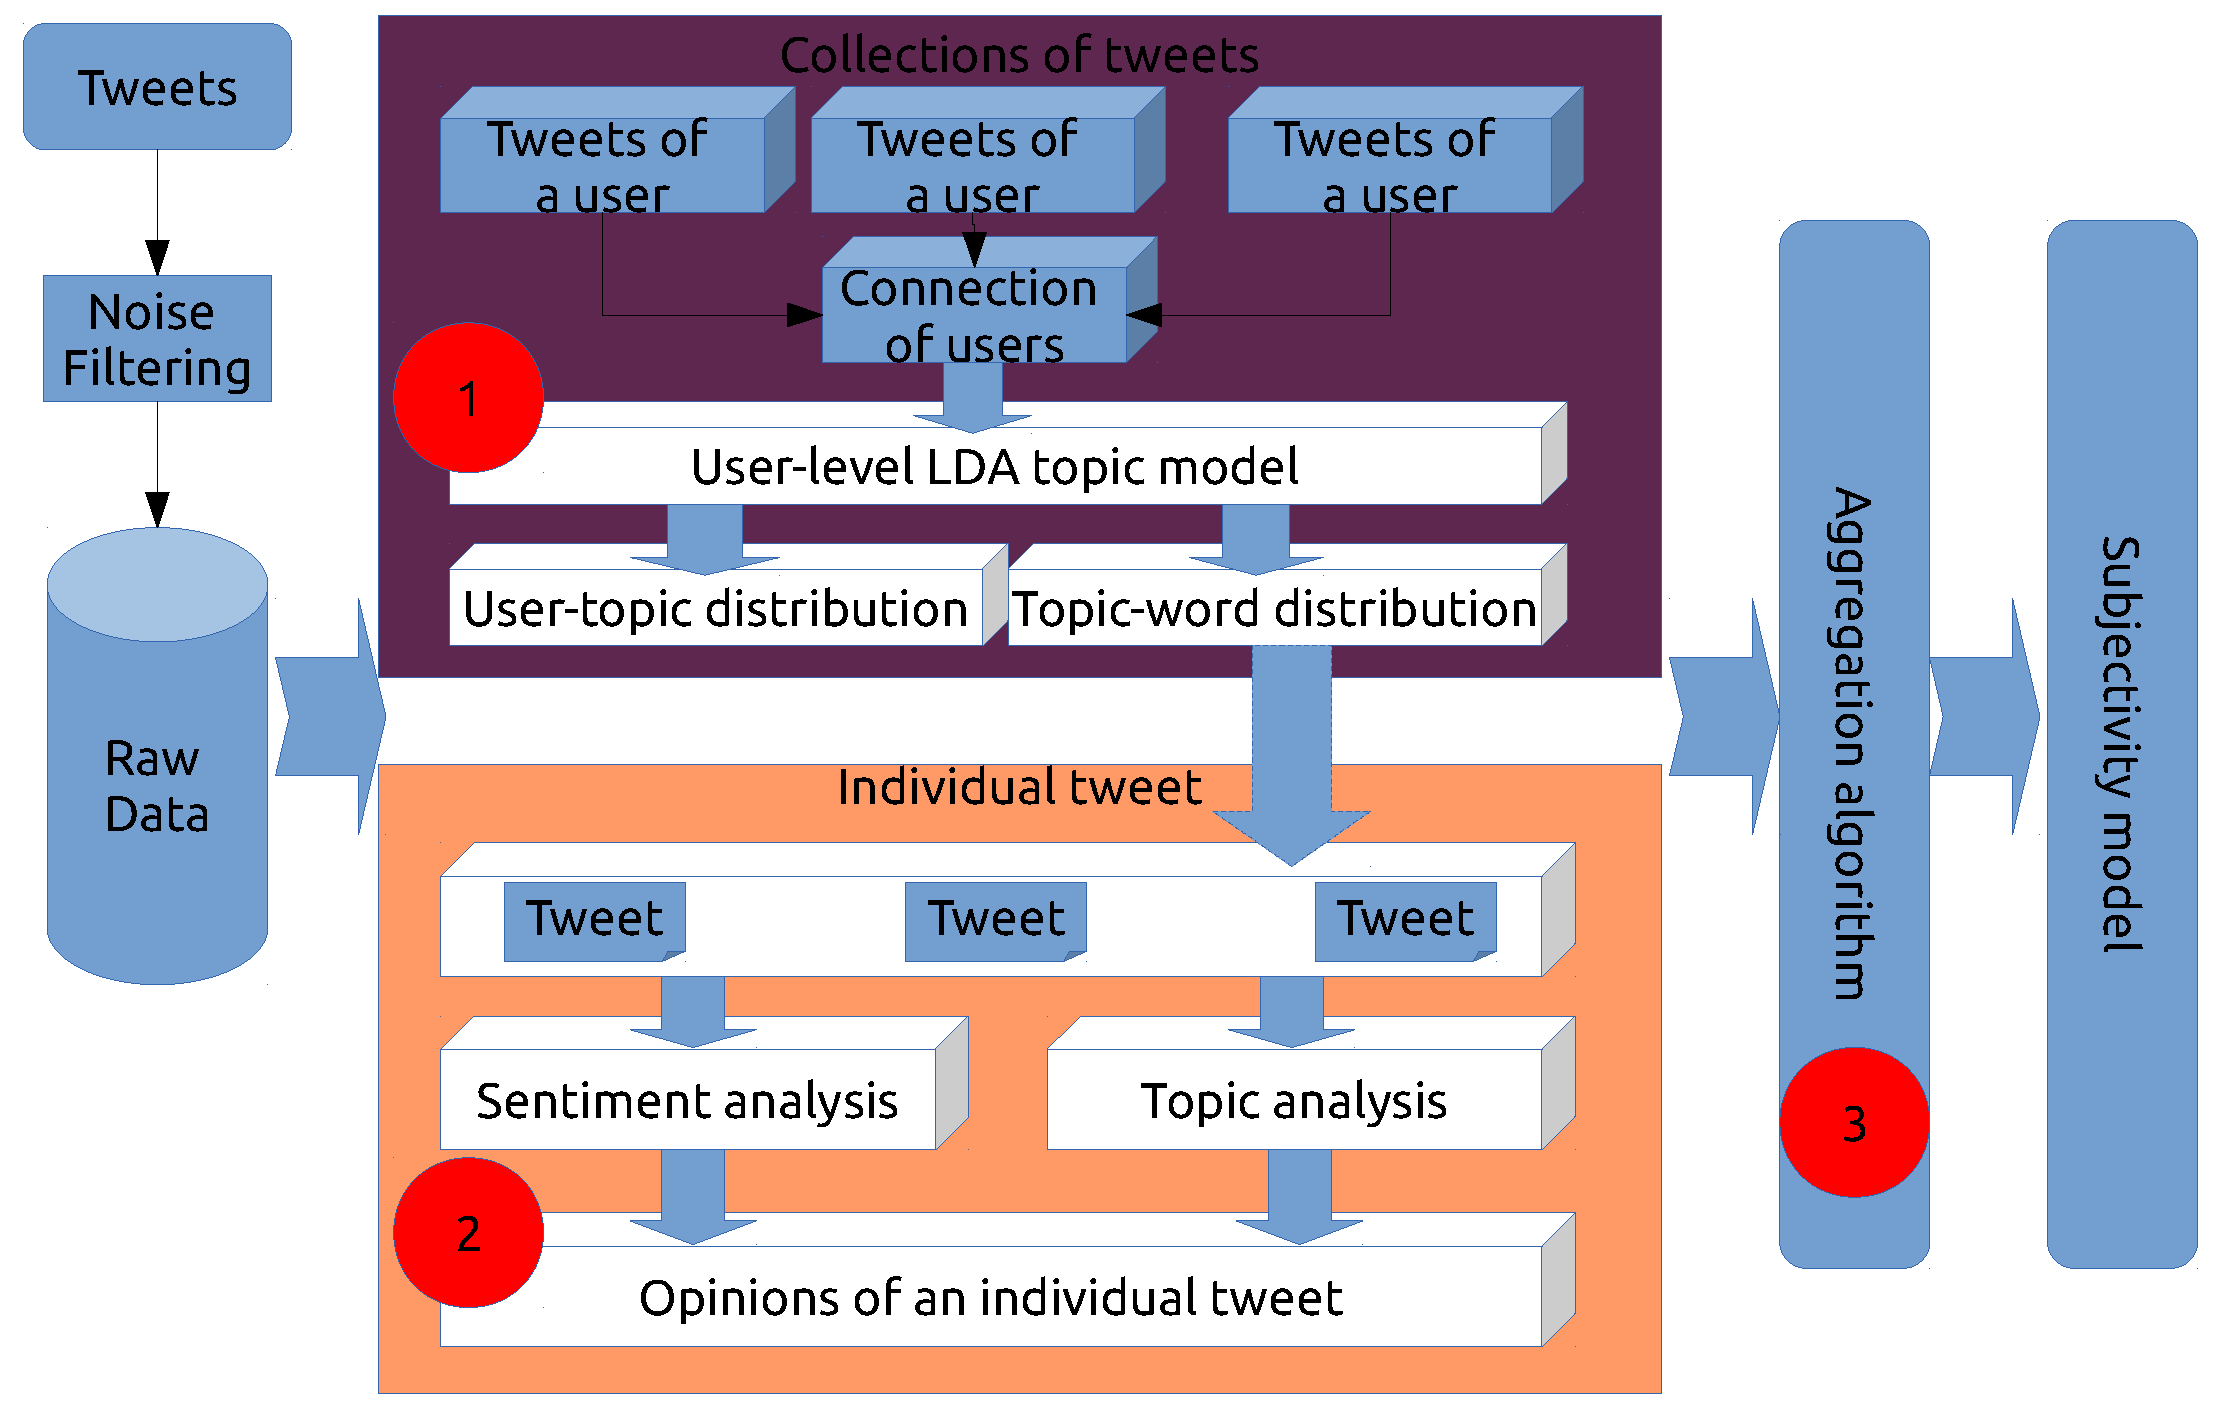
\includegraphics[height=300pt]{5-1.png}
\caption{主观模型总体框架}
\label{fig5-1-1}
\end{figure*}
\end{landscape}

上述这些工作都证明了从用户自己发布的内容中挖掘关键信息的重要性,并且从四方面信息对用户进行建模,即基本信息(“Who you are”),发帖行为(“How
you tweet”),发帖内容(“What you tweet”)以及网络关系(“Who you tweet”),但是少有工作关注于对用户的兴趣和观点进行综合建模,也就是全面反映用户的主观性,本章基于这一动机提出主观模型概念对用户的主观性进行建模。

\section{观点集成问题}
\label{sec3}
如在引言部分所介绍,用户在使用社交媒体平台的时候发布的信息是碎片化的信息,因为用户会在不同的时间就感兴趣的多个话题以及话题多个方面多次发表自己的观点。因此要确定一个用户在某个话题上观点不能只看他的一条信息,应该将他所有与特定话题相关的信息中的表达的观点进行综合才能确定用户的真正观点。为了满足对用户的主观性建模分析需求,在此提出观点集成问题(\textbf{Opinion Integration Problem} (OIP))定义作为用户层面的观点分析的基础。如果站在信息消费者角度,信息使用者主要关注用户层面(User level)的观点信息,而不是单个微博层面(tweet-level)的观点信息,因为观点分析的最终目标是发现人的主观想法而不只是单条微博中的观点信息,对单条微博中观点信息分析只是对分析用户主观性的一个中间步骤。此外,很多情况下用户的单条微博中的观点因为受到长度限制以及上下文语境的缺失常常是不明确的,但是通过用户的所有微博就可以知道其明确的观点信息\upcite{tan2011user}。

本节所提出的话题相关的观点集成问题(OIP)可以用图~\ref{fig5-2}进行说明。
\begin{figure}[htb]
\centering
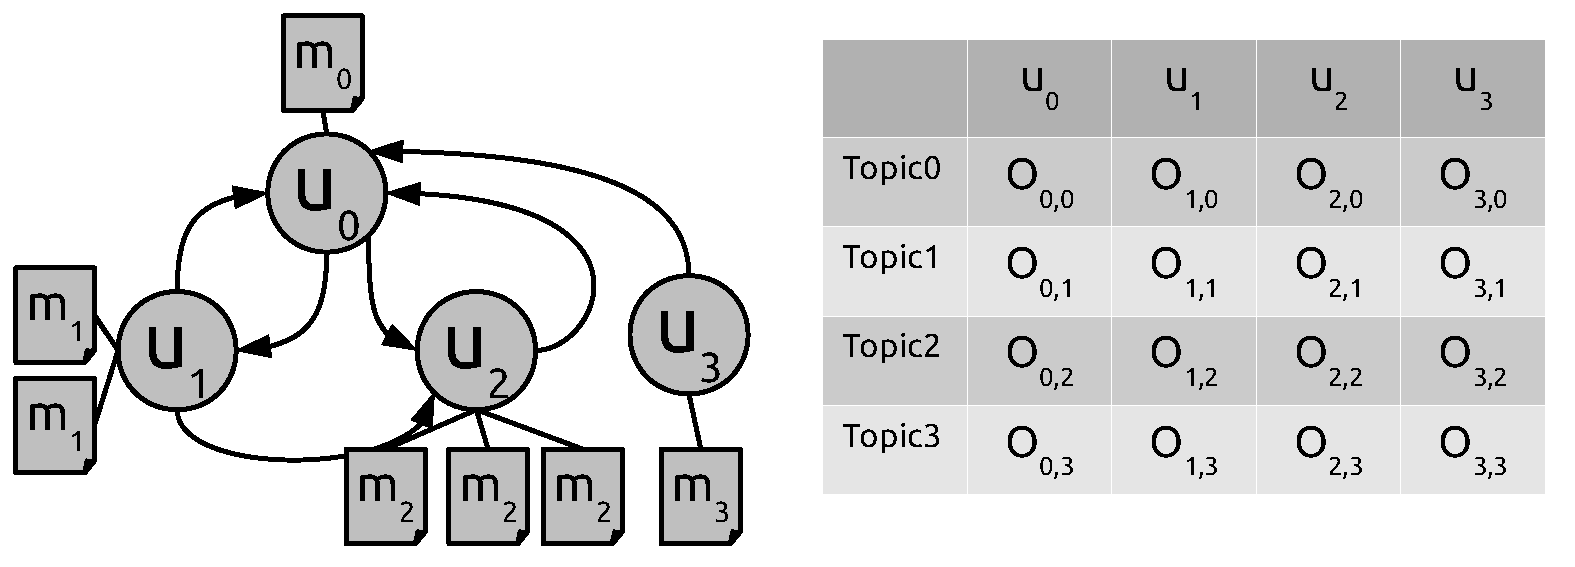
\includegraphics[height=130pt]{5-2.png}
\caption{观点集成问题示例}
\label{fig5-2}
\end{figure}
如图中所示,假设Twitter上的一个异构网络(heterogeneous network)是由用户集合$ V=\left\{ u_{i} \right\} $,用户之间的关系$ E=\left\{(u_{i},u_{j})| u_{i},u_{j} \in V\right\} $以及每个用户$ u_i $发表的微博集合$ M_{i}=\left\{ m_{i} \right\} $构成,其中用户所关注的话题$ T=\left\{ Topic_{j} \right\} $以及用户每条关于话题$ Topic_{j} $微博表达的观点$ o_{i,m,j} $可以从在网络中确定和抽取出来。于是观点集成问题可以定义为:
\begin{definition}[观点集成问题]
用户$ u_{i} $对某一话题 $ Topic_{j} $的观点$ O_{i,j} $不是他某条微博$ m_{i} $表达的观点,应该是从他所有与话题$ Topic_{j} $相关的微博$ M_{i}=\left\{ m_{i} \right\} $中通过某种方法$ f(o_{i,m,j}) $集成得出的,即:$$ O_(i,j)=\sum_mf(o_{i,m,j})$$
\end{definition}

观点集成问题有两个因素必须考虑:首先为了观点所针对目标话题的一致性,异构网络中无论是用户还是微博谈及的话题必须是在同一个话题空间,以使得无论话题的表示形式(比如概念(concept)表示或是话题模型的词袋向量空间的多项式分布表示)还是话题粒度都能够保持一致;其次,也是最重要的,就是集成的观点的表示形式问题,由于观点是与话题紧密相连的,一个用户针对某话题所发表的所有微博会覆盖与话题相关的所有方面,并且对于不同的方面会有不一样的喜好,比如对于手机“iphone”,用户可能喜欢它好看的外观和智能化操作系统,却不喜欢电池的待机时间过短,因此采用什么样的形式表示集成后的观点能准确表达出用户的总体观点是需要考虑的重要问题。下一节将会提出一个主观模型的概念,可以很好满足以上两个要求。

\section{主观模型}
\label{sec4}
其实心理学已经对主观性进行了广泛的研究,并基于个人的历史行为和言论中定义其主观性,以表示独特个性\upcite{Engbert2007}。在语言学上,语言中的主观性定义为作者在发布的文本中所表现出的自己立场、态度和情感\upcite{Stein2005}。社交媒体的出现为用户提供了能够针对感兴趣话题表达自己意见以展现自己独特主观性言论平台,因此在社交媒体平台上,用户的“\textbf{主观性}”可以定义为用户产生内容中涉及的话题和针对话题的表达的观点,因此主观性不但涉及到用户观点,也包含观点针对的目标。

本节首先给出主观模型的形式化定义以满足提出的用户层面观点分析需求。一般来讲,用户层面的观点分析是将用户针对某话题的情感极性分为“积极的(Positive)”或是“消极的(Negative)”。“积极的”情感表示该用户对话题支持或者喜欢,而“负面的”情感表示不支持或不喜欢。本节所提出的主观模型采用了更加通用(General)的“观点”定义,也就是用户针对某话题观点是一个在情感表示空间上的分布,该情感表示空间由可以表示情感强度的情感极性值构成。情感表达空间可以表示更细粒度的观点,因此可以更好的区分细致的观点差别,比如对话题持支持度为8的观点比支持度为5的观点更加具有“积极性”。其实对观点表示形式的定义还没有统一的标准,本节采用这种比较广义的定义是为了能使得主观模型能够更加通用。为了具体讨论问题,下面统一在Twitter平台对主观模型进行定义和分析,其实本章所提出的主观模型可以适用于其他的社交媒体平台。另外,之所以将模型命名为“\textbf{主观模型}”是因为是对社交媒体中用户产生内容中的主观性信息进行建模。

\subsection{模型定义}
\label{definition}
以$G=\left( V,E \right) $表示Twitter上一个异构社交网络,其中$ V $是网络中的用户,$ E\subset V\times V $是用户之间的关注关系(Following relationship)。对于每一个用户$ u \in V $,对应的微博集合 $ M_{u} $表示其发布所有内容。假设在这个社交网络中存在一个话题空间$ T $ 包含了$ V $中所有用户谈论的所有话题,以及一个情感表示空间$ S $用于表示用户观点。
对于用户$ u  \in V $的“\textbf{主观性(subjectivity)}”,定义为用户所发表的所有微博$ M_{u} $中所涉及的话题以及针对话题集成的观点。
  
\begin{definition}[主观模型]
用户$ u $的主观模型$ P \left( u \right) $是用户在话题空间$T$中所谈论话题$\left\lbrace  t \right\rbrace $以及他对每个话题所持有的观点$\left\lbrace O_{t}\right\rbrace $,观点用情感表示空间$ S $上的情感分布表示。
\begin{equation}
\label{usermodel}
P \left( u \right) = \lbrace \left( t, w_{u} \left( t \right), \lbrace d_{u,t} \left( s \right)|s \in S \rbrace \right) |  t \in T \rbrace
\end{equation}
其中:
\begin{itemize}
\item 对于用户$ u $,权重$ w_{u} \left( t \right)$表示其在话题空间中每个话题$t \in T$的兴趣强度,并且$ \sum_{t=1}^{|T|}w_{u} \left( t \right)=1 $。
\item 用户$ u $对话题$t$的观点$O_{t}$指的是对话题所有情感在情感强度空间$ S $的分布$O_{t}=\lbrace d_{u,t} \left( s \right)|s \in S \rbrace $,并且$ \sum_{s=1}^{|S|} d_{u,t} \left( s \right)=1$。
\end{itemize}
\end{definition}

主观模型通过将用户兴趣与观点同时考虑对用户的主观性进行建模,用户兴趣使用一个话题分布表示,对话题的观点用一个情感值的分布表示,主要目标是为了研究用户层面的观点信息,获得用户兴趣和观点比较全面的理解。

\subsection{主观模型的构建}
\label{establish}
根据主观模型的定义,使用了两个分布对用户的主观性进行建模:一个是话题分布,一个是针对每个话题的观点分布,二者都需要从用户发布的历史微博中经过计推理得出。然而对Twitter数据进行内容分析面临一些挑战:Twitter上微博数量十分庞大,但是每条微博由于受限于140字的限制而相对短小,并且各种不规范的语言被广泛使用,缺乏大规模的标注数据等。这些都使得机器学习方法和自然语言处理技术很难以达到好的分析效果\upcite{cambria2014jumping}。
因此能够有效的对Twitter的微博内容进行建模分析需要一些能应对这些挑战并且尽量不使用需要标注数据的方法和技术。为了主观模型的通用性,在设计构建方法时主要考虑使用一些无监督的技术从用户微博中挖掘话题和观点信息,然后通过观点集成来构建用户的主观模型。因此提出一个通用的框架来构建主观模型,该框架的主要优势就是利用Twitter的社交网络结构来帮助应对短文本微博造成的稀疏问题,并使用基于规则以及无监督方法解决无标注数据问题\upcite{Lin2010}。

\subsubsection{话题分析}
\label{topic}
微博所涉及的话题一般是隐性的,需要从微博内容中经过推导得出。目前针对微博话题发现研究主要集中于定位关键词(Key words)\upcite{Chen2010},抽取实体(Entity extraction)\upcite{Abel2011},借助外部知识库(External knowledge categories)\upcite{Macskassy2011},或者使用语义框架(Semantic framework)\upcite{Gangemi2014}等方法。这些方法面临一个主要的问题是数据稀疏问题,因为在谈论同一个话题时,不同用户会使用各种不同的词汇来描述和表达。还有一个重要的方向是各种无监督话题模型,其中LDA话题模型\upcite{Blei2003}及其各种扩展模型\upcite{Weng2010}对微博中的话题分析更加有效\upcite{Hong2010}。LDA模型的话题表示形式在概念上更加宽泛,每一个话题都表示为在所有词空间上的一个分布,因此可以有效应对话题表示的稀疏问题。主观模型的构建框架采用了用户层面LDA话题模型(User-level LDA)从用户所有的微博中发现隐性话题,对应于LDA话题模型,用户层面LDA话题模型生成过程可以使用图~\ref{fig5-1}来表示。

\begin{figure}[htb]
\centering
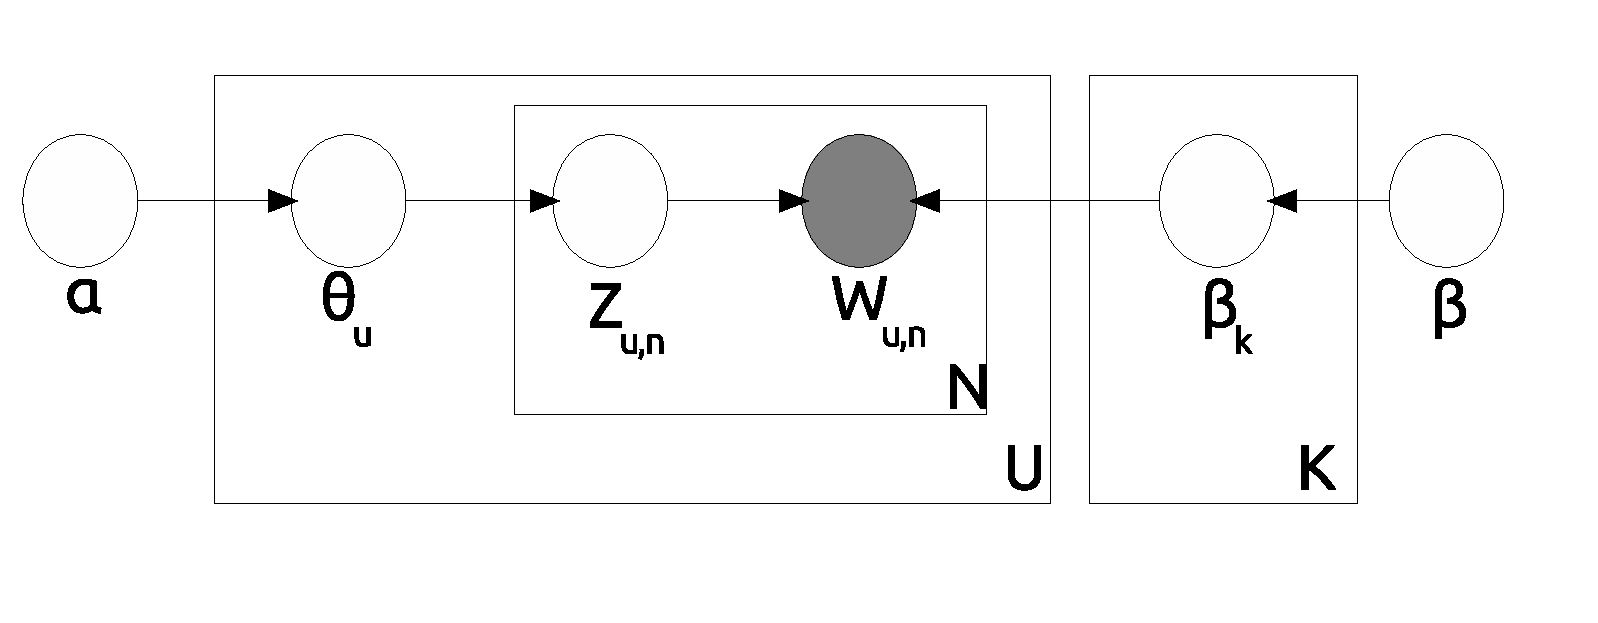
\includegraphics[height=100pt]{5-0.eps}
\caption{用户层面LDA话题模型}
\label{fig5-1}
\end{figure}

具体生成过程如下:
\begin{itemize}
\item 对每个用户$ u $,从先验中获取兴趣话题分布$ \theta_{u} \sim Dir \left(  \alpha \right) $;
\item 对用户微博中的每个词语$ w_{u,n} $,$ n \in \left\lbrace 1, \cdots, N \right\rbrace $:
\begin{itemize}
\item 从用户兴趣话题分布中获取一个话题$ z_{u,n} \sim Multinomial \left( \theta_{u}  \right) $;
\item 根据话题$ z_{u,n} $,从话题的多项分布中获取词语$ w_{u,n} $:$ p \left( w_{u,n} \vert z_{u,n}, \beta_{k}  \right) $。
\end{itemize}
\end{itemize}

为了从用户产生的内容中抽取出涉及的话题,用户产生的微博内容应该和LDA话题模型的文档对应起来。构建主观模型时,主要目标是为了了解用户感兴趣的话题而不是单条微博谈论的过细话题,所以我们将每一个用户的所有微博连接起来组成一篇微博文档作为LDA模型的输入文档。因此用户层面LDA模型中的一篇文档就对应于一个用户,一个用户感兴趣的话题可以使用在话题空间的一个多项式分布来表示,分布的权重可以和主观模型的话题权重相对应。形式化表示为:在用户层面的LDA模型中,给定用户集合$ V $以及话题数目$ K $,一个用户$ u \in V $的所有微博文档可使用话题上一个多项分布$ \theta_{u} $来表示,该分布具有参数为$ \alpha $的Dirichlet先验分布;一个话题$ k \in K $可以用所有词汇上的一个多项分布$ \beta_{k} $来表示,该分布具有参数为$ \eta $的Dirichlet先验分布。模型中的两个分布能够使用Gibbs采样或变分推理(Variational inference)方法进行估计。构建框架中实际本章中我们使用的是基于变分推理的话题模型工具Gensim\upcite{vRehruvrek2010},该工具使用的是在线批处理模式的变分推理方法。

\subsubsection{观点分析}
\label{sentiment}
微博用户经常会通过发表一些跟自己感兴趣话题相关的微博来表达自己的观点,因此为了分析微博用户的主观性,需要了解用户每条微博表达的观点。前面三章内容详细介绍了社交媒体观点分析的各种方法,主要方法可以分为基于规则(词典)方法以及基于机器学习方法两类。如果要准确分析微博观点,基于机器学习方法训练过程需要大量标注数据,Twitter的庞大数据量以及语言的动态性决定了很难对这样的数据进行标注,主观模型的构建优先采用基于规则的方法,基于规则的方法具有很好的灵活性,可以将Twitter的一些语言特点转化成为分析规则,因而更适用于Twitter的观点分析\upcite{Hu2013,Thelwall2010}。

在基于规则的方法中,SentiStrength是专门针对社交媒体中的不规范短文本数据进行情感分析的工具包\upcite{Thelwall2010}。SentiStrength将对应于社交媒体语言特点的规则融合进了基于词典的方法,非常适用于主观模型对Twitter观点分析需求。SentiStrength对每条微博情感分析后输出两个情感值:一个积极极性情感强度值($ [1,5] $范围内)和一个消极极性情感强度值($ [-5,-1] $范围内)。SentiStrength输出的情感值不是简单的积极和消极极性二值结果,而是细粒度的情感强度值,符合主观模型细粒度情感表示空间上分布需求。因此主观模型构建框架使用SentiStrength对所有微博进行情感分析。为了使用方便,将SentiStrength的两个输出结果映射为一个在$ [0, 8] $的离散整数值表示情感强度,映射函数为:
\begin{equation}
\label{opinionmap}
o=\begin{cases} 
{p+3} &  \qquad if \; \vert p \vert > \vert n \vert \\
{n+5} &  \qquad if \; \vert n \vert > \vert p \vert \\
{4}  &   \qquad if \; \vert p \vert = \vert n \vert
\end{cases}
\end{equation}
其中$ p $代表SentiStrength输出的积极极性情感强度值,$ n $代表消极极性情感强度值。与情感极性想对应,在$ [0, 8] $情感表示空间中,强度值4和5表示中性(neutral)情感,强度值大于5表示积极极性,强度值小于4表示消极极性。使用SentiStrength对用户的每条微博进行情感分析的到一个在$ [0, 8] $情感表示空间的情感值,将所有微博的情感值综合,就可以对用户的观点进行集成。

\subsubsection{构建主观模型}
\label{concrete}
对用户微博进行话题分析以及情感分析后,我们就可以为用户开始构建主观模型了。
对于一社交网络的用户集合$ V $,用$ M_{u}=\left\lbrace m_{i} \right\rbrace$表示每一用户 $ u \in V $所发布的所有微博。按照用户层面LDA话题模型要求,将$ M_{u} $中所有微博连接在一起形成一片长的微博文档$ d_{u} $,然后可以用这些微博文档$\{ d_{u}|u \in V\} $使用LDA话题模型进行训练获得话题个数为$ K $的话题空间。
训练得到的话题模型用参数$ \theta $表示每个用户在话题空间$ T $中感兴趣的话题的分布,参数$ \beta $表示每个话题在所有微博词汇上的分布。
使用SentiStrength对每个用户的每条微博$ m $进行情感分析得到每条微博大的情感强度$ s_{m} $。用户主观模型的构建过程可以分为三个步骤:
\begin{enumerate}
\item 在生成的话题模型中,参数$ \theta_u $可以直接对应到用户$ u $在话题空间中的兴趣话题分布,可以确定用户感兴趣话题为:
\begin{equation}
\label{eq5-1}
Z_u=\{t|p(t|\theta_u(t))>0,t \in T\}
\end{equation}
\item 将话题模型应用到用户$ u $每条微博$ m $确定涉及话题为:
\begin{equation}
\label{eq5-2}
Z_m=\{t|p(t|\theta,\beta,m)>0,t \in T\}
\end{equation}
\item 对用户$ u $发布的所有涉及话题$ t $的微博观点进行集成分析的到用户在话题上的观点:
\begin{equation}
\label{eq5-3}
O_{t} = \left\{ \frac{N_{s}}{\sum_{s \in S} N_{s}} |s \in [0,8] \right\}
\end{equation}
其中$ N_s =\sum_{m \in M_{u}} I\left( s_{m} \right) $($s_{m}=s \& t \in Z_{m} $)表示用户发布的涉及话题$ t $情感值为$ s $微博数目。

最后综合形成用户主观模型:
\begin{equation}
\label{subuser}
P(u)= \left\lbrace \left( t, p\left( t \vert \theta_{u} \right), \left\{ \frac{N_{s}}{\sum_{s \in S} N_{s}} \right\}  \right)  \vert t \in Z_{u}, s \in S  \right\rbrace
\end{equation}
\end{enumerate}

对用户$ u $构建主观模型$ P(u) $的详细过程如算法~\ref{alg5-1}所示:

\begin{algorithm}[htb] 
\caption{主观模型的构建过程} 
\label{alg5-1}
\begin{algorithmic}[1] %这个1 表示每一行都显示数字
\REQUIRE ~~\\ %算法的输入参数:Input
用户集合$ V $;\\
每个用户所发布的微博集合 $ M_{u} $;\\
\ENSURE ~~\\ %算法的输出:Output
为每个用户$ u $构建的主观模型 $ P(u) $;
\STATE 使用用户层面的话题模型对用户微博内容分析获得模型 $P(\theta,\beta|M_{u},V)$; 
\label{ alg1:topic }%对此行的标记,方便在文中引用算法的某个步骤
\FORALL {用户每条微博 $ m \in M_{u} $}
\label{alg1:sentiment}
\STATE 对 $ m $情感分析获得情感值 $ s_{m} $;
\ENDFOR
\FOR {每个用户$ u \in V$}
\STATE 用户感兴趣话题分布为参数$ \theta $对应的分布 $ \theta_{u} $;\\
\STATE 使用公式~\ref{eq5-1}确定用户话题集合$ Z_{u}$;
\ENDFOR
\FOR {每条微博 $ m \in M_{u} $}
\STATE 使用公式~\ref{eq5-2}对微博$ m $话题分析,得到微博涉及话题$ Z_m $;
\ENDFOR
\FOR {用户每个兴趣话题$ t \in Z_{u} $ }
\FOR {情感表示空间的每个情感值$ s \in S $}
\STATE 统计用户$ u $发布的微博中情感值为$ s $且涉及话题$ t $的数目$ N_{s}$;
\ENDFOR
\STATE 使用公式~\ref{eq5-3}计算用户$ u $对话题$ t $的集成的观点分布$ O_t $;
\ENDFOR
\STATE 构建用户$ u $的主观模型$  P(u)$;
\RETURN $P(u)$ %算法的返回值
\end{algorithmic}
\end{algorithm}

以上的构建方法中,由于微博话题的集中性,简单假设微博$ m $的情感$ s_m $是针对微博所涉及的所有话题$ Z_{m} $,并没有区分针对不同话题的不同情感。

\subsection{与生成模型比较}
\label{comparison}
在情感分析领域,一些研究提出了基于话题模型的话题情感模型,能够扩展基本的话题模型将文档中表达的情感与话题相结合统一建模\upcite{Mei2007,Lin2009}。其中TSM模型(Topic Sentiment Mixture model)\upcite{Mei2007}认为文档中表示情感等主观信息的词语与描述话题的词语是相互独立的,因此可以将表示情感的语言模型跟表示话题的语言模型分开建模,在文档的生成过程中任一词语的生成或者从话题语言模型中采样获得,或者从情感语言模型中采样获得,二者只能选择一个。JST模型(Joint Sentiment/Topic model)\upcite{Lin2009}提出了一种新的方式来分析文档中的情感信息,在话题模型抽取话题过程中将话题和情感关联起来,因此可以同时对话题和情感信息联合建模。
这些模型在发现话题相关的情感极性时跟本章提出的主观模型是很相似的,都能同时对用户的感兴趣话题以及话题相关的主观性信息建模。

但是这类模型通常假设存在一个词语-情感分布,需要通过学习获得这个通用词语-情感分布来对文档中的情感知识建模,这对短小和不规范社交媒体语言,尤其是Twitter来说是很困难的。相对于话题的表达,情感、观点等主观信息更难识别,因为情感信息常常隐式的存在于一些微妙的语言表达方式中(比如反讽),并且一些具体的领域和语境中也会具有独特的情感表达方式。微博中的情感除了一些正规语言的表达方式外,还有很多微博特有的语言来表达,比如表情符、字母大小写变化、不规范词语中字母重复强调以及惊叹号等标点符号的使用等等。微博上的这些语言特点表达出的情感很难用词语-情感概率分布表示。但是基于规则的情感分析方法可以很容易通过设计规则反映这些特有语言特点,用规则获取微博语言中微妙的情感表达方式。因此,主观模型构建中采用了基于规则的情感分析工具发现微博中的情感信息,更适合于Twitter等短文本社交媒体上用户主观性的建模。

\subsection{主观模型的应用}
\label{application}
从用户微博中学习得到的主观模型能够应用到用户观点分析以及行为(转发、关注等行为)分析中。本节以用户观点的预测为例来验证主观模型的作用,也就是学习到的主观模型能否有效的对用户将来针对某话题的观点进行预测。根据用户观点的一致性,假设用户不会就某一话题随机表达积极或消极极性观点,例如一个支持某候选人的用户更趋向于针对该候选人发表正面观点的微博。社会学上称这种现象为人的主观偏执(bias),也就是人的主观性\upcite{Walton1991}。因此得到了用户的主观模型,可以根据用户前期表现出的主观性预测用户就某一话题发表的微博所持观点。

首先将这种观点预测问题形式化为三元组$ < author, m, t >$,其中$author$是微博$ m $作者,微博涉及话题为$ t $。观点预测的目标就是通过计算得出用户$author$的微博$ m $针对话题$ t $表达出的观点极性$ p=\left\{positive,negative\right\} $。情感分析领域针对这一问题的主要方法是从微博中抽取出文本的情感表达模式,然后利用这些模式来预测观点的极性。
单条微博经常会由于缺乏上下文信息而使得观点具有模糊性,用户的主观模型是从用户所有的历史微博中构建的,因此有丰富的上下文信息,并且根据用户主观性的一致性假设,主观模型中对某一话题的观点比一条微博中的观点更加稳定一致。因此可以使用主观模型来提高用户未来发表微博中观点预测效果。
具体来说,对微博$ m $,其作者的主观模型可以根据算法~\ref{alg5-1}构建,假设作者新发布的微博为$ m $,$ m $的情感值通过某种方法比如SentiStrength分析得出为$s_m$,并且$ m $所涉及话题可以使用的公式~\ref{eq5-4}推导得出:
\begin{equation}
\label{eq5-4}
\hat{t}=argmax(\hat{P}(t| \theta,\beta ,Z_{u})|t)
\end{equation}

用户$author$在话题$ \hat{t} $上的观点分布可以从主观模型$ P(author) $中确定为$ O_{author,\widehat{t}} $,是一个在情感表示空间$ S $上的分布,因此可以计算出用户在话题$ \hat{t} $上归一化情感值:
\begin{equation}
\hat{s_{m}}=\sum_{i \in T}d_{i}\ast v_{i}
\end{equation}
其中$ v_{i} $表示情感值,$ d_{i} $表示情感值对应的分布。

于是可以使用微博情感分析得到的情感值$s_m$和主观模型计算出的情感值$ \hat{s_{m}} $联合进行观点极性$ p $预测:

\begin{equation}
\label{polarity}
p=  
\begin{cases}
{positive} &  \qquad if \; \dfrac{\hat{s_{m}}+s_m}{2} > \dfrac{|S|}{2} +1\\
{negative} &  \qquad if \; \dfrac{\hat{s_{m}}+s_m}{2} < \dfrac{|S|}{2} \\
{neutral}  &   \qquad otherwise \;  
\end{cases}
\end{equation}

\section{实验}
\label{sec5}

\subsection{数据集及设置}
实验使用的数据集是通过Twitter公开API抓取的数据集\upcite{Li2012a},数据集的具体规模如表~\ref{tab5-1}所示。

\begin{table}
\centering
\caption{Twitter数据集统计}
\label{tab5-1}
\begin{tabular}{|l|l|l|l|}
\hline
项目 & 规模 & 项目 & 规模\\
\hline
总用户数& 139,180 & 每个用户平均朋友数& 14.8 \\
\hline
总连接数 &  4,175,405 & 每个用户平均粉丝数 & 14.9  \\
\hline
总微博数 & 76,409,820 & 每个用户平均微博数 & 549 \\
\hline
\end{tabular}
\end{table}

由于LDA模型的计算复杂度,直接从139,180个用户的所有微博中构建主观模型需要大量时空开销。根据社交网络的同质性(Homophily)\upcite{Lazarsfeld1954},也就是“物以类聚(Birds of a feather flock together)”的原则\upcite{McPherson2001},社交网络中连接紧密的用户更趋向于讨论相同话题,持有相似观点\upcite{Thelwall2010a}。在Twitter上,用户之间的连接关系对应着用户间的认可或关注关系,还意味着拥有有相似话题或观点。因此可以利用社交网络的连接紧密用户形成的社区结构(community),将139,180个用户划分为不同的社区,在社区内部为用户构建主观模型,这种利用社交网络结构特点化整为零的方法,可以降低构建主观模型的计算复杂度。实验使用Igraph\footnote{\url{http://igraph.org/}}工具包划分社区,最后将用户划分为106个社区。对于用户数少于15的小社区,使用LDA模型进行话题分析效果比较差,因此实验中将这些社区和用户过滤,同时也过滤掉了发微博少于5的、每次发微博字数少于5个的还有微博内容只有url连接的用户总共15,756个。最后形成的数据集中有122,329个用户,分部于33个社区中。每个用户在其社区内局部网络中按照算法~\ref{alg5-1}构建主观模型。

除了主观模型,实验也将主观模型与两个话题情感生成模型JST和TSM进行了对比试验。所有模型的Dirichlet先验参数设为$ \alpha=50/T $($ T $为话题数目),$ \beta=0.01 $。JST的不对称情感先验参数$ \gamma $依照经验设为$ (0.01, 1.8) $。JST和TSM模型推导都经过了2,000次迭代Gibbs采样。

\subsection{样例分析}
为了定性展主观模型表达用户主观性能力,在此给出了使用本章提出框架构建的一个用户的主观模型如图~\ref{fig5:a}和~\ref{fig5:b}所示。该用户发表了533条微博,所有微博可以用词云图\footnote{实验使用TagCrowd (\url{http://tagcrowd.com/})生成词云图。}~\ref{fig5:a}来展示。

\begin{figure}[htb]
\centering
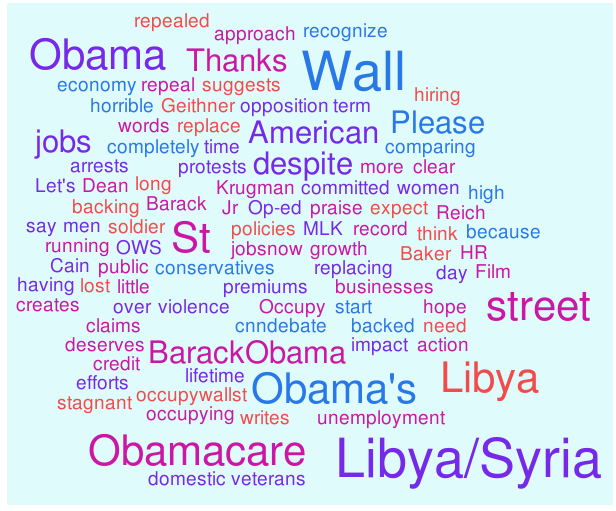
\includegraphics[height=220pt]{5-4.png}
\caption{微博词云}
\label{fig5:a}
\end{figure}

\begin{figure}[htb]
\centering
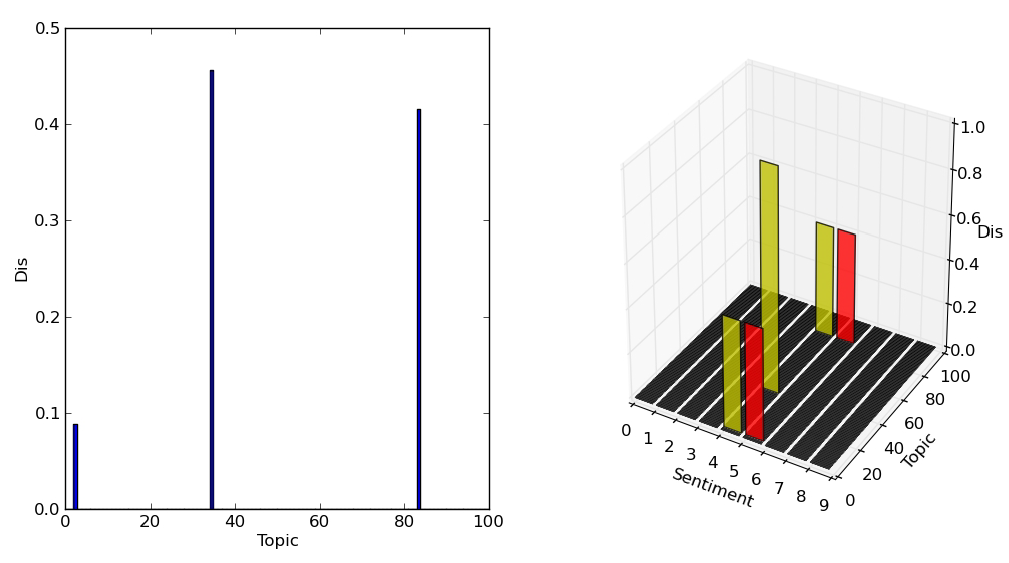
\includegraphics[height=200pt]{5-3.png}
\caption{主观模型样例}
\label{fig5:b}
\end{figure}

图~\ref{fig5:b}\footnote{主观模型中,左侧图代表话题分部: $ (  w_{u}\left( 2 \right)=0.08,w_{u}\left( 32 \right)=0.48, w_{u}\left( 83 \right)=0.44)  $;右侧图代表观点的分部: $ O_{2}=( d_{u,2} \left( 4 \right)=0.5, d_{u,2} \left( 5 \right)=0.5)$, $O_{32}=(d_{u,32} \left( 4 \right)=1.0) $, $ O_{83}=( d_{u,83} \left( 4 \right)=0.5, d_{u,83} \left( 5 \right)=0.5 ) $。}是用户在$ [0,100] $话题空间和$ [0,8] $情感表示空间中可视化的主观模型。很明显,从词云图上可以看到该用户讨论了三个话题(话题2:``\#Obamacare'',话题32:``\#libya''以及话题83:``\#occupywallst''),图~\ref{fig5:b}左侧展示了用户在每个话题上的兴趣权重。图~\ref{fig5:b}右侧是用户对这三个话题所持观点分布,总体来看,对于话题``\#libya''情感分布100\%在强度4上,属于中性,对话题``\#Obamacare''和``\#occupywallst''情感分部都是50\%在强度4以及50\%在强度5上,属于中性偏积极极性。从这个样例可以看出,主观模型对用户的主观性进行了细致的建模,不但有用户的兴趣分布,也有细粒度的观点分布信息。

\subsection{观点预测性能}
为了定量评价主观模型的性能,主观模型在观点预测任务上与两个话题情感模型(TSM和JST)以及几个常用的情感分析方法进行了对比实验。由于缺少可用的标注数据,实验中主要跟几个无监督的情感分析方法进行了对比,这些方法主要有:
\begin{itemize}
\item \textbf{OF:OpinionFinder}是一个公开可用的情感分析软件包,主要是用于句子层面的主观性分析\upcite{Wilson2005}。
\item \textbf{S140:Sentiment140}使用远距离监督(distant supervision)方式(使用表情符获取训练数据)进行微博的情感分类的在线工具。
\item \textbf{STR:SentiStrength}将微博中的一些语言特点转化成规则,并结合基于情感词典方法,专门针对微博等社交媒体短文本进行情感分析工具\upcite{Thelwall2010}。
\end{itemize}

实验从数据集中随机选择了1,000个至少有80条微博的用户,然后选择每个用户按照时间顺序发布的最后一条微博组成了1,000条测试数据集。所有的1,000条微博进行人工标注作为评测标准。话题模型的话题数分别设置为50, 100, 150以及200,评价指标使用的是准确率,结果如表~\ref{tab5-2}所示。

\begin{table}[htb]
\centering
\caption{观点预测对比实验结果}
\label{tab5-2}
\begin{tabular}{|l|l|l|l|l|}
\hline
情感分类方法 & 50 & 100 & 150 & 200\\
\hline
OF &  65.85\%& & & \\
\hline
S140 &  70.45\%& & & \\\hline
STR &  69.98\%& & & \\\hline
TSM & 63.46\%& 72.94\% $ \ast $  &67.83\% & 66.65\% \\\hline
JST & 61.25\% & 68.57\% $ \ast $ & 75.88\%  $ \ast $ & 67.03\%\\\hline
SUB & 71.53\% $ \ast $ & 81.05\% $ \ast $ & 78.32\% & 74.54\%\\
\hline
\end{tabular}
\begin{tablenotes}
  \centering
  \footnotesize
  \item 相对于OF显著的性能提升使用$ \ast $标记。\\
\end{tablenotes}
\end{table}

从表中可以看出:
\begin{itemize}
\item 首先,OpinioFinder的准确率是最低的65.85\%,主要原因是OpinioFinder主要是针对评论而设计的情感分析工具,不适用于Twitter这种语言环境;
\item 其次,两个无监督情感分析方法Sentiment140和SentiStrength因为是专门针对Twitter设计,准确率都明显好于OpinionFinder(Sentiment140:70.45\%,SentiStrength:69.98\%);
\item 第三点,总体上两个话题情感生成模型TSM和JST的准确率都好于OpinioFinder,并且准确率都比Sentiment140和SentiStrength方法稍好(但是不显著),证明了将情感信息与话题分析相关联的重要性;
\item 最后,主观模型(SUB)准确率在四种话题设置下准确率都显著地好于三个无监督情感分析方法,并且将主观模型计算出的情感值与SentiStrength对微博情感值想结合后,显著提高了SentiStrength准确率,与两个话题情感生成模型相比较,主观模型性能明显比TSM要好,稍好于JST,这是因为主观模型构建所用的情感分析方法更适合与Twitter语言,能够更准确的分析微博中的情感信息。
\end{itemize}

\section{小结}
\label{sec6}
本章中,针对用户层面的观点分析,定义并研究了社交媒体中用户的观点集成问题,提出了主观模型概念并进行可形式化定义,主观模型中定义了通用观点表示形式,使得主观模型可以在更细粒度的情感表示空间中对用户的观点进行集成,将集成的观点表示为情感表示空间的分布;提出了基于规则和无监督方法构建主观模型的框架,该框架采用新的算法从用户的历史微博中抽取话题和观点信息,得到的话题分布对用户的兴趣建模,将同一话题微博中的观点信息集成为一个观点分布对用户在话题上的观点建模;使用真实Twitter数据对主观模型进行了定性和定量评测,实验结果证明,主观模型能有效的对用户的主观性进行建模,并且在观点预测任务中基于主观模型的方法性能显著比现有的几个情感分析方法要好,而且比TSM和JST两个话题情感生成模型更适应Twitter上用户的主观性建模。
%\newpage 
%\mbox{} 
%\newpage
\chapter{用户转发行为分析}
\label{ch6}

\section{引言}
\label{ch6_intro}
上一章介绍了如何从社交媒体用户产生内容中挖掘出话题和观点信息并在用户层面集成对用户的主观性进行建模,本章主要介绍如何应用主观模型对用户在信息传播中的转发行为进行分析。

信息传播通过逐步层叠式的信息扩散触发大量用户参与到信息的病毒式传播中,在市场营销、政治选举等应用场景中发挥着重要作用,引起了众多研究者,尤其是社交网络研究人员的广泛关注。社交网络研究为信息传播设计了一些通用的传播模型,可以进行模拟信息流动(Information flow)\upcite{Goldenberg2001,Kempe2003}以及探测信息瀑布(Information cascades)爆发\upcite{Cheng2014}。但是这些模型都是将用户看作是网络中的一个简单节点,忽视了用户在信息传播过程中的行为自主性。作为社交媒体中的信息消费者和产生者,每个用户都可以在社交媒体上发帖和转贴以表达自己的兴趣和观点,能自主选择信息和传播信息。在社交媒体中一条信息能否得到广泛传播主要依赖于用户间的“口碑(Word of mouth)”效应,只有口碑效应好的信息才会引起广泛用户的兴趣对其进行传播,口碑效应取决于用户信息消费的主观意图,因此分析用户的主观意图可以对促进信息的传播研究。随着自然语言处理(Natural language processing)和数据挖掘(Data mining)技术的发展,社交媒体用户的主观意图可以使用用户自己产生的数据进行建模来分析。本章就是基于口碑效应机制问题,研究给定某个用户的一条微博,分析所有收到该微博用户中谁最有可能参与到该条微博的后续传播中。一个典型的场景是,在如图~\ref{fig6-0}所示Twitter的一个异构网络中,用户Tony和关注他的所有朋友在以往的信息交流中讨论了两个话题:“苹果手机(Iphone)”以及电影“冰雪奇缘(Frozen)”,要研究的问题是:Tony新发布了一条有关电影“冰雪奇缘”微博,如何判定他所有朋友中谁会转发传播这条微博?

\begin{figure}[htb]
\centering
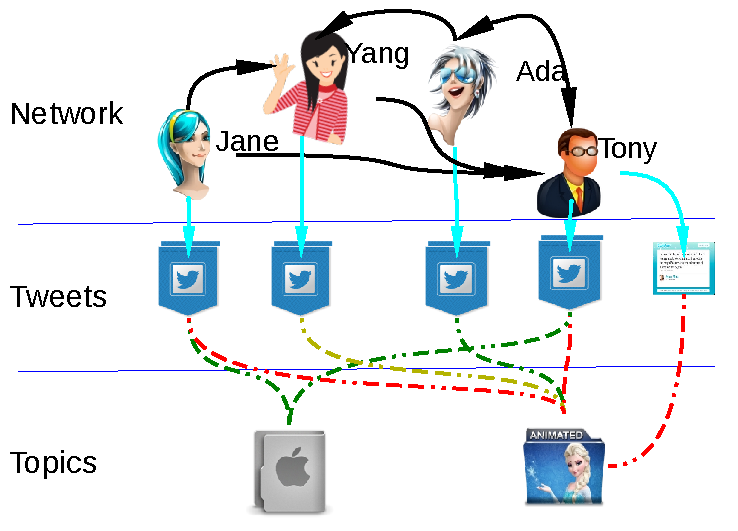
\includegraphics[height=180pt]{6-0.pdf}
\caption{问题示意图}
\label{fig6-0}
\end{figure}
%\footnotetext{每个用户的观点用不同颜色表示,“红色”当标正面观点,“绿色”代表负面观点,“黄色”代表中性观点。}

不同社交网络平台上的信息传播行为是不一样的,本章主要分析Twitter用户的微博转发行为。庞大的用户群以及信息的指数级增长,使得Twitter在互联网的信息传播中扮演着重要角色。尽管Twitter微博在长度上受到限制,但是Twitter提供用户间转发机制为信息的快速传播提供了前所未有的便捷途径。据有关统计,Twitter中有超过四分之一的微博是由用户间的相互转发形成的\upcite{yang2010understanding},因此理解了用户的转发行为就能够很好的解释Twitter上的信息传播。

社交媒体用户是信息传播的参与者,同时也是个性化的信息消费和生产主体,用户很自然地会在信息的交互中表达出自己兴趣和观点,表现出主观性。在心理学的研究中证实了人的主观能动性(Subjective initiative)决定了人的主观性会影响自己的行为模式\upcite{Moore2008},同样根据偏颇吸收(Biased Assimilation)理论,人总是趋向于选择跟自己偏执化观点(Biased opinions)相一致的信息进行传播\upcite{Hyman2000}。因此用户的主观性是研究用户参与信息传播意图的一个很重要的方面。转发行为分析研究提出了一些方法和模型来确定一些影响转发行为的因素\upcite{Macskassy2011,Feng2013}。但是目前还没与相关工作关注到用户转发行为的主观动机。从Twitter的口碑效应来看,转发行为是一个连续的过程,包含着接收到微博,对微博内容评估,最后确定时候转发三个环节。三个环节中最重要的就是评估微博内容是否有价值的信息值得和朋友分享,也就是用户转发行为的主观动机。因此对用户的主观动机进行建模会为转发行为分析提供重要的研究视角。依据“物以类聚(Like attracts like)”原则,用户更容易转发那些能够迎合他个人口味的信息。以图~\ref{fig6-0}中的例子来说明,每个用户对网络中谈论的两个话题所持观点可以从他们历史发布的微博中得出,假设Tony和Jane对电影“冰雪奇缘”持正面肯定观点,而Ada持负面观点,Yang持中性观点。如果Tony新发布的微博内容是对冰雪奇缘表达正面肯定的观点,应该可以确定Jane是最有可能转发这条微博的用户。从这种动机出发,本章主要研究用户的主观性是如何影响其转发行为。

为了研究主观性和转发行为的关系,需要回答两个问题:(1)怎样准确对用户的主观性进行建模?(2)怎么样从用户的主观性角度度量微博值得传播?
上一章内容已经提出了使用观点集成方法来对社交媒体上用户主观性建模,并定义了社交媒体用户的主观模型及其构建方法。本章将继续使用主观模型概念,并针对用户的转发行为分析提出一个新的主观相似性计算方法来度量微博是否值得传播,针对影响转发行为的三个因素,即微博内容的吸引力、转发行为的社交需求以及从众需求(Conformity needs)\upcite{Cialdini2004},定义三个主观相似性度量三个因素对转发行为的影响。

\section{相关工作}
\label{ch6_relatedwork}
在微博转发行为分析方面,已经有大量工作在转发行为特征分析、提高微博转发性因素确定以及设计模型估计转发概率三个方面展开研究。例如Suh等~\upcite{suh2010want}发现带有Url网络连接以及hashtag标记的微博更有可能被转发;Macskassy和Michelson~\upcite{Macskassy2011}发现从微博内容中推理得到的模型能够解释大多数的转发行为;Comarela等\upcite{comarela2012understanding}发现与微博作者前期交互,微博作者发帖频率,微博内容的新鲜程度以及微博的长度会影响关注者的转发行为;Starbird和Palen~\upcite{starbird2012will}特别针对危机发生时的微博信息转发机制进行了研究,发现有危机话题关键词的微博更有可能被转发;Osborne和Lavrenko~\upcite{petrovic2011rt}通过引入一些特征,比如微博的新颖性和作者被加入朋友列表的次数,使用被动攻击算法(Passive aggressive algorithm)训练模型预测转发行为;Jenders等~\upcite{jenders2013analyzing}从微博及其作者的网络结构、信息内容以及情感信息分析了一些“显式”和“隐式”的影响转发的特征;Naveed等~\upcite{NaveedGKC2011,naveed2011searching}
引入了微博的趣味性指标,并使用表情符、情感以及话题等特征对趣味性指标进行量化来预测微博被转发的可能性;Feng和Wang~\upcite{feng2013retweet}构建了一个图模型,并将微博以及用户的所有信息组合到图的节点和边的信息里面,并提出了一个因子分解模型(Factorization model)对微博依据被转发的概率进行排序;Pfitzner等~\upcite{Pfitzner2012}提出了一种叫做情感分歧(emotional divergence)指标来评价微博被转发的可能性,并研究证实了高情感分歧值的微博会有更高的机会被转发;Luo等\upcite{Luo2013}设计了包括转发历史特征、用户特征、用户活跃时间特征以及用户兴趣特征四组特征集合对用户转发微博行为进行分析,并根据转发可能性对用户排序。

总体来说,上述所有工作主要是回答“哪些微博会否被什么样的用户转发”这样一个问题,但是忽略了用户在转发时的主观动机,也就是“站在用户角度,某条微博是否值得用户转发”这样的问题,本章将结合上一章提出的主观模型从用户用户的主观动机角度来分析转发行为。

\section{基于主观模型的转发分析}
为了研究用户转发行为的主观动机,首先需要了解用户的主观性,也就是弄清楚用户喜欢什么和不喜欢什么(即用户感兴趣的话题和用户对话题所持的观点),这就是上一章为用户所建立主观模型的用途,通过用户主观模型可以清楚了解用户的主观性,为分析用户的转发行为分析提供信息基础。从技术角度来讲,上一章提出的主观模型的目标就是设计一个通用的框架能够从社交媒体用户产生历史数据中同时获得用户兴趣(对应的话题分布)和全面的观点(对应的观点分布)信息,为后续的一些应用提供信息支持。之所以主观模型是通用的,因为它不但将用户的兴趣和观点结合进一个整体框架,更重要的是,在主观模型中观点表示为一个在可扩展的情感表示空间上的概率分布。这个情感表示空间既可以是表示情感正负极性的二值空间,又可以是连续值表示的情感强度空间,或是离散值表示的情绪类型空间,因此可以覆盖所有的观点表示形式。这种观点的表示形式一方面可以在细粒度的情感值空间区别不同观点,另外一方面可以以概率分布计算不同观点之间的相似性,能够准确区分观点和判断观点相似性是对用户主观动机分析的基础。本节主要定义主观相似性为转发行为的主观动机分析提供有效的度量手段。


%随着社交媒体普及率越来越高,社交媒体上带有用户主观性信息的用户产生内容(UGC)也越来越多,自然语言处理领域的观点挖掘(opinion mining)\upcite{Liu2012}研究开始通过计算方式自动对用户的观点信息进行建模。并且也出现了一些基于方面(aspect-based)情感分析或话题情感模型(topic-sentiment model)\upcite{Lek2013,Mei2007}将针对话题的观点投射为二值极性,评价等级或情绪类型等某一个单一的情感值,但是这些模型因为这种观点简单的表示形式而使得其作用受到限制。因此在主观模型中,我们通过将话题和观点结合为一个模型并将话题和观点使用新的表示形式(在话题空间和情感空间的分布)来对用户的主观性进行建模。

\subsection{主观相似性}
\label{similarity}
%Twitter用户一般会对感兴趣的多个不同话题发表观点和看法,比如图~\ref{fig6-0}中的例子中Tony和Jane都对苹果手机话题和冰雪奇缘电影感兴趣并表达了自己的观点。
%一般来讲,用户对话题的兴趣度会随着话题的不同而不同,而且,即便对同一个感兴趣话题,当一个用户其其不同的方面(aspects)发表微博表达的观点也不是完全一样的,因此我们认为对用户的主观性进行建模时:
%\begin{itemize}
%\item 每一个用户$ u $都对应着一个在话题空间$ T $的$ |T| $维的话题分布$ W_{u}=\{w_u(t)\}|W_u \in R^{|T|},\sum_{t}w_{u}(t)=1 $,其中$ w_{u}(t) $表示用户在话题$ t $上的兴趣度。
%\item 用户$ u $对话题$ t $的观点应该表示为一个在情感空间$ S $的$ |S| $维的情感分布$ O_t=\{d_{u,t}(s)| O_t \in R^{|S|}, \sum_{s}d_{u,t}(s)=1\}$,其中$ d_{u,t}(s) $表示用户观点中带有情感值$ s $的可能性。
%\end{itemize}


%图~\ref{fig6-1}是一个在$ [0,100] $话题空间和$ [0,8] $情感强度空间主观模型的可视化示例。
%
%\begin{figure}[htp]
%\centering
%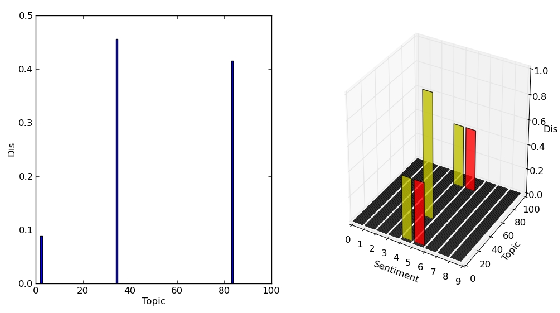
\includegraphics[height=170pt]{6-1.pdf}
%\caption{可视化主观模型示例}
%\label{fig6-1}
%\end{figure}
%左侧图中表示用户在话题2,32和83上的兴趣度:$$ (  w_{u,2}=0.08,w_{u,32}=0.48, w_{u,83}=0.44)  $$
%右侧图中表示在每个话题上的观点分布:
%$$ O_{2}=( d_{u,2,4} =0.5, d_{u,2,5} =0.5)$$
%$$O_{32}=(d_{u,32,4}=1.0) $$ $$O_{83}=( d_{u,83,4}=0.5, d_{u,83,5}=0.5 )$$

构建主观模型框架是将话题分析和观点分析分开进行的。具体来讲,首先使用用户层面(user-level)的LDA话题模型从用户所有的微博$M_u$中训练一个全局话题模型$ TM=(\theta,\beta) $,其中$ \theta $表示用户在话题空间$ T $的兴趣度分布,$ \beta $表示话题在词表上的分布。由于微博比较短小,通常认为每条微博谈论的是一个话题,因此可以通过计算微博$ t $从话题模型中产生的概率值,为$ t $指定一个最有可能的话题:
\begin{equation}
\label{eq6-1}
z_{t} = \arg \max_{k}\prod_{w \in t} P(w|\phi_{k})
\end{equation}

然后就可以将用户$ u $所有谈论同一话题的微博数目进行归一化后获得用户在话题上的兴趣度:
\begin{equation}
w_{u,k}=\dfrac{|\{ t: t \in M_{u} \wedge z_{t}=k\}|}{|M_{u}|}
\end{equation}

至于观点的分布式表示,正如在图~\ref{fig6-0}中的例子,虽然Tony和Jane总体上都是对电影“冰雪奇缘”持正面观点,但是他们有可能是因为不同的原因而喜欢这部电影的。Jane可能非常喜欢电影浪漫的故事情节,但是对它的动画画面稍微有点失望;而Tony喜欢这部电影可能是因为被这部电影的动画技术所折服,却不喜欢它略显幼稚的公主王子题材。情感分析研究主要是将观点表示为单一值,尤其是正负极性二值为主,并不区分针对话题的观点在不同方面的具体观点,也无法计算观点的大小顺序,比如那个用户更喜欢电影。在主观模型中,观点被定义为在情感表示空间$ S $的概率分布,可以更精确的表示和区分观点。假设微博$ t $通过情感分析得出情感值为$ s_t $,用户在某一话题$ k $上的观点分布可以将所有谈论该话题微博在每一个情感值上的数量归一化后获得:
\begin{eqnarray}
O_k &= & \{ d_{u,k,s}|s \in S \} \nonumber \\
  &=& \{ \dfrac{|t:t \in M_u \wedge z_t=k \wedge s_t=s|}{|M_u|}|s \in S\}
\end{eqnarray}

为了量化“物以类据(like attracts like)”这样的效应,得到用户的主观模型后,需要定义一个相似性度量方法来计算用户之间或用户与微博之间主观上的相似性。首先定义在同一话题上两种观点的相似性计算方法。
 
\subsubsection{观点相似性}
\label{opsim}

在主观模型中观点是定义在情感空间上的分布,分布的每一维都代表着在对应情感值上的观点权重。为了区分观点,可以定义情感表示空间中的情感值不独立,情感值之间按照一定的顺序和大小来表示情感的强度。比如情感值为8的观点比情感值为5的观点持更正面的观点。这种情况下常用的一些计算分布相似性的方法,比余弦相似性(cosine similarity)以及KL距离(KL-divergence),对于主观模型中观点分布相似性的计算就不适合。例如表~\ref{tab6-1}所示的三个观点分布,代表在一个$ S=[0,8 ] $情感表示空间中的三个观点:观点$ O_{k}^{1} $是最负面(100\%分布在情感值0上),观点$ O_{k}^{2} $是正面的(50\%分布在情感值6,50\%分布在情感值7上),观点$ O_{k}^{3} $最正面(100\%分布在情感值8上)。
\begin{table}[htb]
%\scriptsize
\centering
\caption{观点相似性示例}
\label{tab6-1}
\begin{tabular}{|l|l|l|l|l|l|l|l|l|l|}
\hline
 观点& 0 & 1& 2 & 3 & 4 & 5 & 6 & 7 & 8 \\
\hline
$O_{k}^{1}$ & 1.0 & 0.0 & 0.0 & 0.0 & 0.0 & 0.0 & 0.0 & 0.0 & 0.0 \\
\hline
$O_{k}^{2}$ & 0.0 & 0.0 & 0.0 & 0.0 & 0.0 & 0.0 & 0.5 & 0.5 & 0.0 \\
\hline
$O_{k}^{3}$ & 0.0 & 0.0 & 0.0 & 0.0 & 0.0 & 0.0 & 0.0 & 0.0 & 1.0 \\
\hline
\end{tabular}
\end{table} 

使用常规的分布相似性计算方法(余弦相似性或KL距离),就会发现三个观点之间的相似性都是0,因而出现了相似性计算方法失效现象,这是与实际不相符的,因为观点$ O_{k}^{2} $与观点$ O_{k}^{3} $比观点$ O_{k}^{1} $与观点$ O_{k}^{3} $更相似,它们都是持正面观点。因此观点的相似性计算不能简单将观点视为一般的概率分布来计算,或者只是情感表示空间的一个距离值。为了准确计算观点之间的相似性,需要将观点在情感表示空间的距离和分布上的相似性结合起来,在此提出了如下的计算观点$O_{k}^{u},O_{k}^{v} $之间相似性方法:
\begin{equation}
\label{opinionsim}
Sim(O_{k}^{u},O_{k}^{v})=\dfrac{|S|-|\sum_{i=0}^{|S|}d_{i}^{u}v_{i}-\sum_{i=0}^{|S|}d_{i}^{v}v_{i}|}{|S|}
\end{equation}
其中$ d_{i} $是第$ i^{th} $维的情感值上的分布,$ v_{i} $是相应的情感值。
使用方法~\ref{opinionsim}计算表~\ref{tab6-1}中观点之间相似性为:
$$ Sim(O_{k}^{1},O_{k}^{3})=0 $$ 
$$Sim(O_{k}^{2},O_{k}^{3})=6/8$$
$$ Sim(O_{k}^{1},O_{k}^{2})=2/8 $$
计算结果达到了与三个观点之间相似性的直觉理解一致的效果。

\subsubsection{主观相似性}
在主观模型中,用户感兴趣的话题表示为在话题空间$ T $上不同话题的兴趣度分布,因此两个主观模型$SM_u$和$SM_v$之间的主观相似性可以将话题上的权重与对应的观点分布相似性结合起来进行集成计算:
\begin{equation}
\label{subsim}
Sim(SM_{u},SM_{v})=\sum_{k=1}^{|T_{u,v}|}\theta_{u}(k)\* Sim(O_{k}^{u},O_{k}^{v})
\end{equation}
其中$ T_{u,v} $表示两个用户之间的共同话题,是两个用户之间感兴趣话题的交集;$ \theta_{u}(k) $代表用户$ u $在话题$ k $上的兴趣度权重。

值得注意的是,当测量用户$ u $在主观性上与用户$ v $有多相似性时,话题权重使用的是用户$ u $的话题权重,因此这个主观相似性度量方法是不对称的。之所以这样设计,是因为考虑到用户的主观上的相似性是个人主观判断,因此度量目标用户与自己主观想法上有多相似是根据个人的话题兴趣度以及观点相似性来确定的,不需要目标用户也作对称性的考量。因此在度量两个用户的主观相似性时,$ Sim(SM_u,SM_v)\neq Sim(SM_v,SM_u)$。

\subsection{转发行为分析}
\label{retweet}
用户的转发行为受到多种因素的影响,从用户的角度来讲,三种情形下会引发用户的转发:
\begin{enumerate}
\item 微博的内容对用户具有吸引力,因此用户的转发行为是根据自己的主观判断引发的;
\item 微博是由关系密切的好朋友发布的,因此用户的转发行为是因为社交需求;
\item 微薄内容是突发新闻或有趣段子,具有流行性,因此用户的转发行为是趋同需求(或称为从众需求,conformity needs)\upcite{Cialdini2004}的结果。
\end{enumerate}
这三种因素是用户产生转发行为的不同原因,从主观动机角度分析,可以使用三个主观相似性来量化这三个因素,从而对转发行为进行分析。

在以下的分析中,对于一条微博$ t $,假设$ F $表示该微博作者$ u_{a} $的所有关注者,当作者$ u_{a} $发布微博$ t $后,所有用户$ f \in F $都会看到微博$ t $,至于哪个用户会转发该微博,需要分析用户的主观动机。对于每一个关注者$ f \in F $,可以定义一个四元组$ <f, u_{a}, t, r_{f}>  $,其中$ r_{f} $是一个二值标签用以表示微博$ t $是否会被用户$ f $转发,需要通过分析进行预测。

\subsubsection{吸引力度量}
一般来讲,用户根据自己的主观判断,看到一个有吸引力的微博就会转发。因此可以通过计算微博$ t $与微博关注者$ f $之间的主观相似性来定量地度量这种吸引力。对于一条微博,它所讨论的话题$ z_t $可以使用公式~\ref{eq6-1}指定,对其进行情感分析可以得到情感值$ s_t $,因此微博也能够使用主观模型进行建模,它的话题分布和观点分布都是一个100\%的单值分布。于是微博$t$对于用户$f$的吸引力就可以使用我们定义的主观相似性计算方法~\ref{subsim}进行度量:
\begin{equation}
Sim(f,t)=\theta_{f}(z_t)\* Sim(O_{z_t}^{f},O_{z_t}^{t})
\end{equation}

\subsubsection{社交性度量}
这种情形下,转发行为是基于用户的社交需求。由于微博是由志同道合(like-minded)的好朋友发的,转发行为是因为友谊触发而不一定是微博$ t $的内容。这种情况下可以通过计算用户$ f $与微博作者$ u_a $之间的主观相似性来度量二者之间友谊的亲密程度:
\begin{equation}
Sim(f,u_a)=\sum_{k=1}^{|T_{u,v}|}\theta_{f}(k)\* Sim(O_{k}^{f},O_{k}^{u_a})
\end{equation}

同时也应该考虑到,不同类型的朋友对用户$ f $的影响力(influence)是不同的,比如用户$ f $可能会关注很多人,但是可能只会与少数几个互动频繁(转发等互动)。而且用户$ f $并不是对关系亲密朋友的每条微博都感兴趣,例如在图~\ref{fig6-0}中的例子中,Jane可能会对Tony所发的关于电影“冰雪奇缘”的微博感兴趣,但是对他的关于苹果手机微博不感兴趣。因此需要对用户之间的主观相似性$ Sim(f,u_a) $附加一个权重以反映不同类型朋友对用户$ f $的影响力,该权重由反应朋友类型和亲密程度的四部分因子组合而成。

\paragraph{专家指数因子(Expert Factor) $ w_E(u_a) $}: 
该因子代表着微博作者$ u_a $在微博接收的朋友圈中相对专家指数,专家指数越高的用户就会对其他用户有更多的影响力。在此只是简单地根据用户$ u_a $的发帖数量在朋友圈中所有用户发帖总数的比例来计算专家指数。
\begin{equation}
w_E(u_a)=|M_{u_a}|/|\{M_u|u \in u_a \cup F \}|
\end{equation}

\paragraph{领导力因子(Leadership Factor) $ w_L(u_a) $}: 
此处简单将用户的领导力影响定义为该用户拥有的粉丝(followers)数。因此领导力因子可以通过归一化计算为:
\begin{equation}
w_L(u_a)=\log (|F|)/\log(\max)
\end{equation}
其中$ \max $是Twitter中用户的最大流行度(maximum popularity)\footnote{\url{http://twittercounter.com/pages/100}}。

\paragraph{相似性因子(Similarity Factor) $ w_S(u_a,f) $}: 
用户$ u_a $和$ f $之间的兴趣的相似性可以通过他们主观模型中话题分布之间的反KL距离(inverse KL-divergence)来度量:
\begin{equation}
w_S(u_a,f)= 1/KL(\theta_{u_a},\theta_f)
\end{equation}

\paragraph{交互因子(Interaction Factor) $ w_I(u_a,f) $}: 
用户$ u_a $和$ f $之间的交互数量$ Interation_{u_a,f} $包括他们之间的对话,相互之间的提及以及相互之间的转发等。该因子可以通过对$Interation_{u_a,f}$使用用用户$ u_a $和$ f $所有的微博数目归一化计算获得:
\begin{equation}
w_I(u_a,f)=|Interation_{u_a,f}| /|\{ M_{u_a}, M_f \}|
\end{equation}

综上所述,将以上四个因子组合后可以得到影响权重:
\begin{equation}
\begin{split}
w_{u_a,f}= \lambda_1*w_E(u_a)+\lambda_2*w_L(u_a)+
  \lambda_3*w_S(u_a,f)+\lambda_4*w_I(u_a,f)
\end{split}
\end{equation}
其中$ \lambda_i $是一个权重向量以反映不同因子的影响,并且$ \sum_{i=1}^{4}\lambda_i=1 $。本章中将其均衡设为$ \lambda_i=0.25 $。

\subsubsection{流行性度量}
用户在使用Twitter时,如果发现一条微博$ t $是非常流行的(具有突发性、新颖性或传染性),在趋同效应或从众心理的作用下,用户很有可能会对其进行转发。这种情形下,微博$ t $的内容一般在话题和观点上与其作者$ u_a $的主观性不太一致,因此微博$ t $与其作者$ u_a $之间的主观相似性$ Sim(u_a,t) $会相对较低:
\begin{equation}
Sim(u_a,t)=\theta_{u_a}(z_t)\* Sim(O_{z_t}^{u_a},O_{z_t}^{t})
\end{equation}
用户的转发行为是由于微博$ t $的流行性而不是其因为内容具有吸引力或者是好朋友发布的,为了度量其流行性影响,需要对$ Sim(u_a,t) $增加一个流行性系数,该系数可以通过计算接收微博$ t $的用户$ f $所关注朋友中转发微博$ t $的比例来确定。

\section{实验}
\label{experiments}

\subsection{数据集与实验设置}
实验使用了Luo等\upcite{Luo2013}研究工作中使用的Twitter数据集\footnote{下载地址:\url{https://sourceforge.net/projects/retweeter/}},在构建数据集时,作者使用Twitter Streaming API随机选取了500条目标微博,每条微博至少被其作者的粉丝转发过一次,对这500条微博进行连续几个小时的监控找到转发微博的那些用户。同时以这500条微博为入口,收集了微博作者及其粉丝的最近发布的200条历史微博。最后得到的数据集总共有45,531个用户,共6,277,736条微博,在监控期间有5,214个用户转发了500条微博中的至少一条。为了避免数据不平衡带来的影响,从数据集中采样抽取了5,214个没有转发目标为博的用户作为反例,与转发者一起构成平衡测试数据集。数据集的具体统计如表~\ref{tab6-2}所示:
\begin{table}[htb]
\centering
\caption{数据集统计}
\label{tab6-2}
\begin{tabular}{|l|c|}
\hline
项目 &数量\\
\hline
监控的目标微博数 & 500 \\
\hline
每条目标微博的平均粉丝数 & 89 \\
\hline
收集到的所有用户数 & 45,531 \\
\hline
所有历史微博数 & 6,277,736 \\
\hline
目标微博的所有转发者 & 5,214 \\
\hline
目标为博所有未转发者 & 40,317  \\
\hline
\end{tabular}
\end{table}

在构建主观模型过程与上一章一样,使用了Gensim\upcite{vRehruvrek2010}进行话题模型训练,话题数目设为50,100,150和200;使用SentiStrength\upcite{Thelwall2010}对每条微博进行情感分析,并且为了更好的适应于微博情感表达方式,采用了Nielsen等\upcite{Mohammad2013}为Twitter构建的情感词典。

\subsection{相关性检验}
首先,为了验证主观相似性时候与转发行为之间存在相关性,实验采用了ANOVA(Analysis of Variance)\upcite{Fisher1970}假设性检验方法对用主观相似性表示的三个因素与转发行为之间的相关性进行分析,使用该检验方法对“\textbf{转发者(retweeters)和非转发者(non-retweeters)具有相同的主观相似性均值}”这一零假设(null hypothesis)进行检验。
结果如表~\ref{tab6-3}所示,表中加黑部分表示\textit{p-value}低于显著性水平。

\begin{table}[htb]
\scriptsize
\centering
\caption{ANOVA检验结果} 
\label{tab6-3}
\begin{threeparttable}
\begin{tabular}{|c|c|c|c|c|}
\hline
\multicolumn{2}{|c|}{相似性指标}& $ Sim(f,t) $ & $ Sim(f,u_a)  $ & $ Sim(u_a,t)  $\\
\hline
\multirow{2}{*}{50} & \textit{F} & \textbf{12.182} & 2.212 & 4.236 \\
\cline{2-5}
  & \textit{p} &  $\mathbf{4.44e^{-06}}$  & 0.140 & 0.272\\
\hline
\multirow{2}{*}{100} & \textit{F} & \textbf{43.892} & \textbf{31.145} & \textbf{28.466} \\
\cline{2-5}
  & \textit{p} &  $\mathbf{8.65e^{-11}}$  & $\mathbf{3.55e^{-08}}$ & $\mathbf{1.32e^{-09}}$\\
\hline
\multirow{2}{*}{150} & \textit{F} & \textbf{22.356} & \textbf{12.240} & \textbf{14.664} \\
\cline{2-5}
  & \textit{p} &  $\mathbf{2.43e^{-08}}$  & $\mathbf{6.25e^{-06}}$ & $\mathbf{8.46e^{-07}}$\\
\hline
\multirow{2}{*}{200} & \textit{F} & \textbf{31.675} & \textbf{20.616} & 6.145\\
\cline{2-5}
  & \textit{p} &  $\mathbf{4.22e^{-06}}$  & $\mathbf{2.92e^{-05}}$ & 0.26\\
\hline
\end{tabular}
\begin{tablenotes}
%  \centering
  \footnotesize
\item 表中如果平均值差异是偶然,\textit{F-ratio}=1.00,否则\textit{F-ratio} \textgreater 1.00 (\textit{p-value} \textless 0.01)。\\
\end{tablenotes}
\end{threeparttable}
\end{table}

从表中可以看出,当话题数是100和150时,所有的主观相似性检验都是\textit{F-ratio}大于1.00,且\textit{p-values}低于显著性水平。这表示所有的主观相似性与转发行为具有相关性,能够作为转发行为的有用特征。后续实验将话题数目固定为100来进行讨论。

\subsection{样例分析}
\label{example}
为了定性说明主观模型在转发行为分析中的作用,首先用一个实际样例来进行阐述。在此从500条目标微博中选取了其中的一条,其内容为:
\begin{description}
\item Sometimes the right person for you was there all along. You just didn’t see it because the wrong one was blocking the sight.
\end{description}

微博作者以及两个关注者(一个是转发者,一个是未转发者)构建的主观模型如图~\ref{fig6-2}所示。

\begin{figure}[htb]
\centering
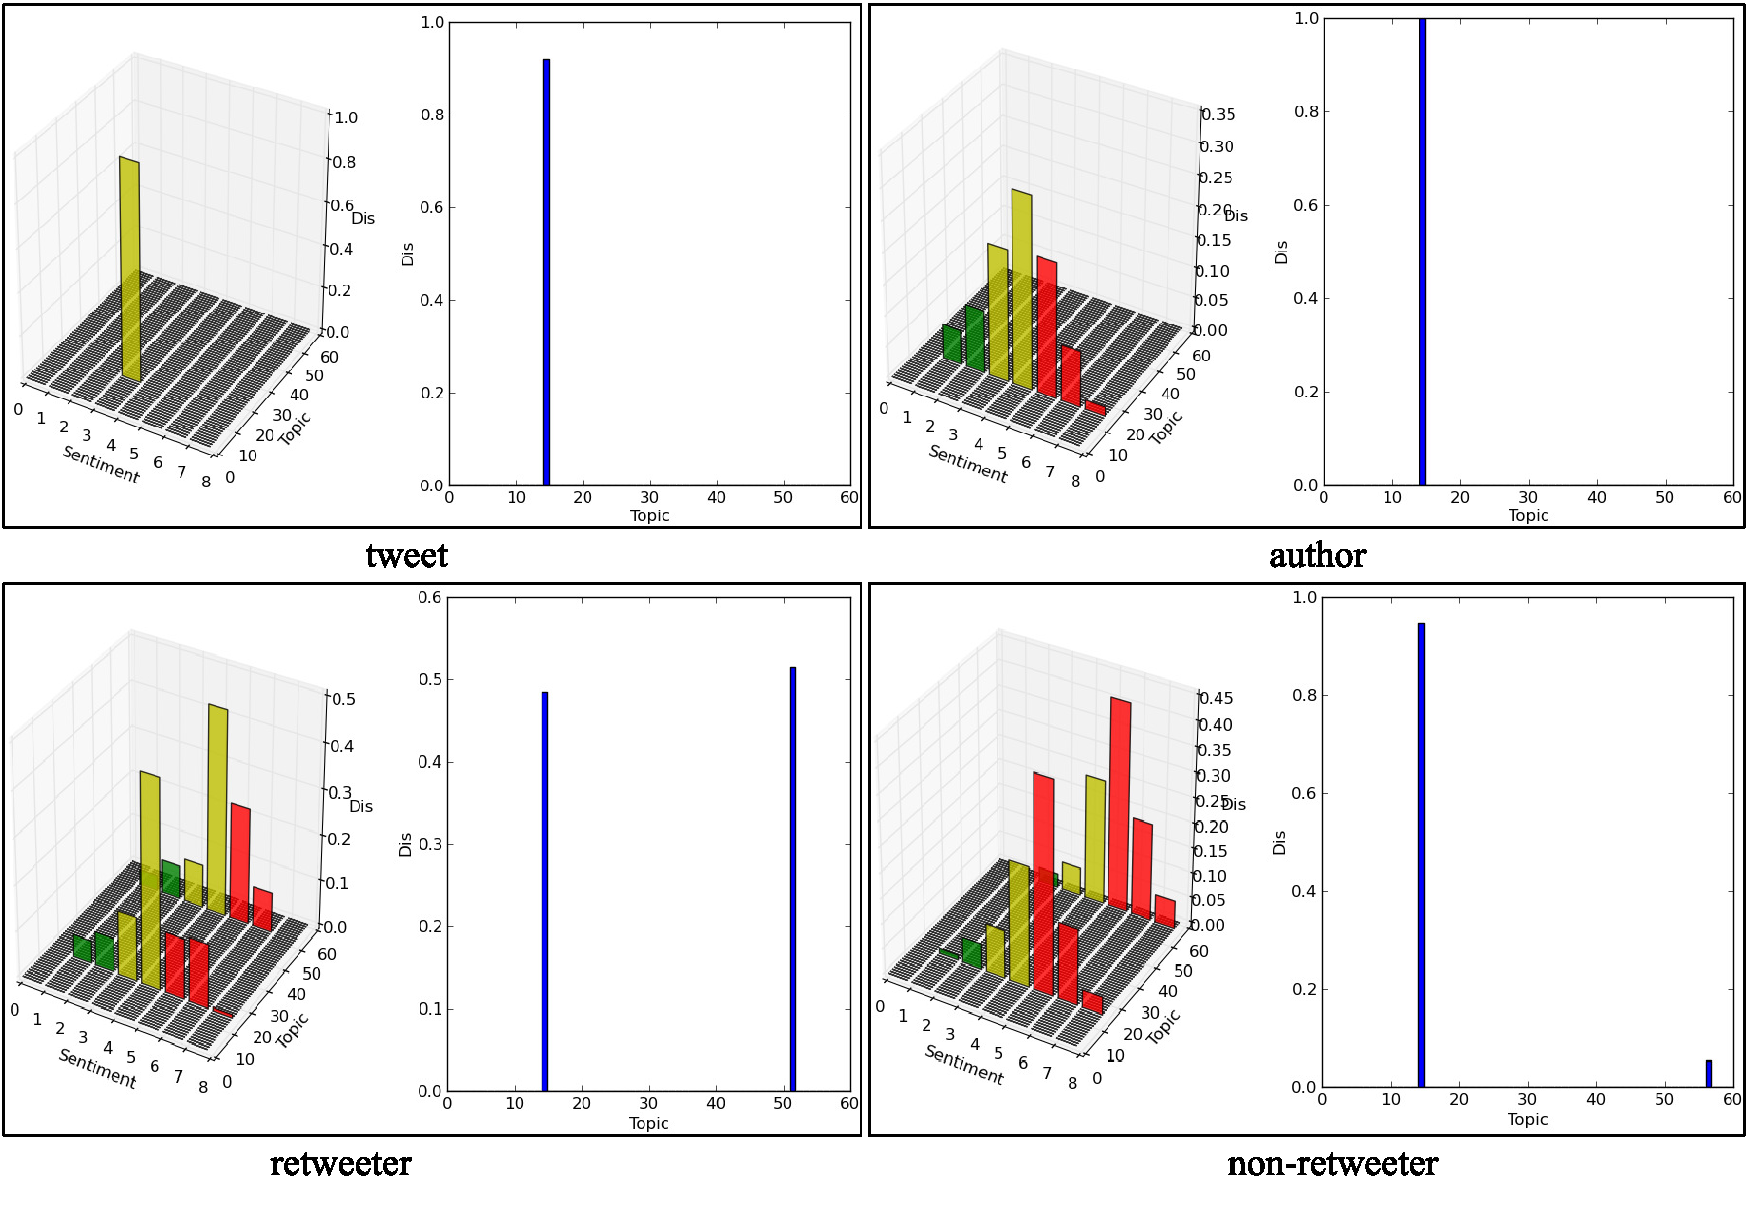
\includegraphics[height=320pt]{6-2.pdf}
\caption{主观模型示意图}
\label{fig6-2}
\end{figure}

图~\ref{fig6-3}显示了$ 14^{th} $号话题、微博作者与两个关注者的所有微博的词云图(word cloud diagrams)\footnote{我们使用TagCrowd (\url{http://tagcrowd.com/})生成词云图。}。

\begin{figure}[htb]
\centering
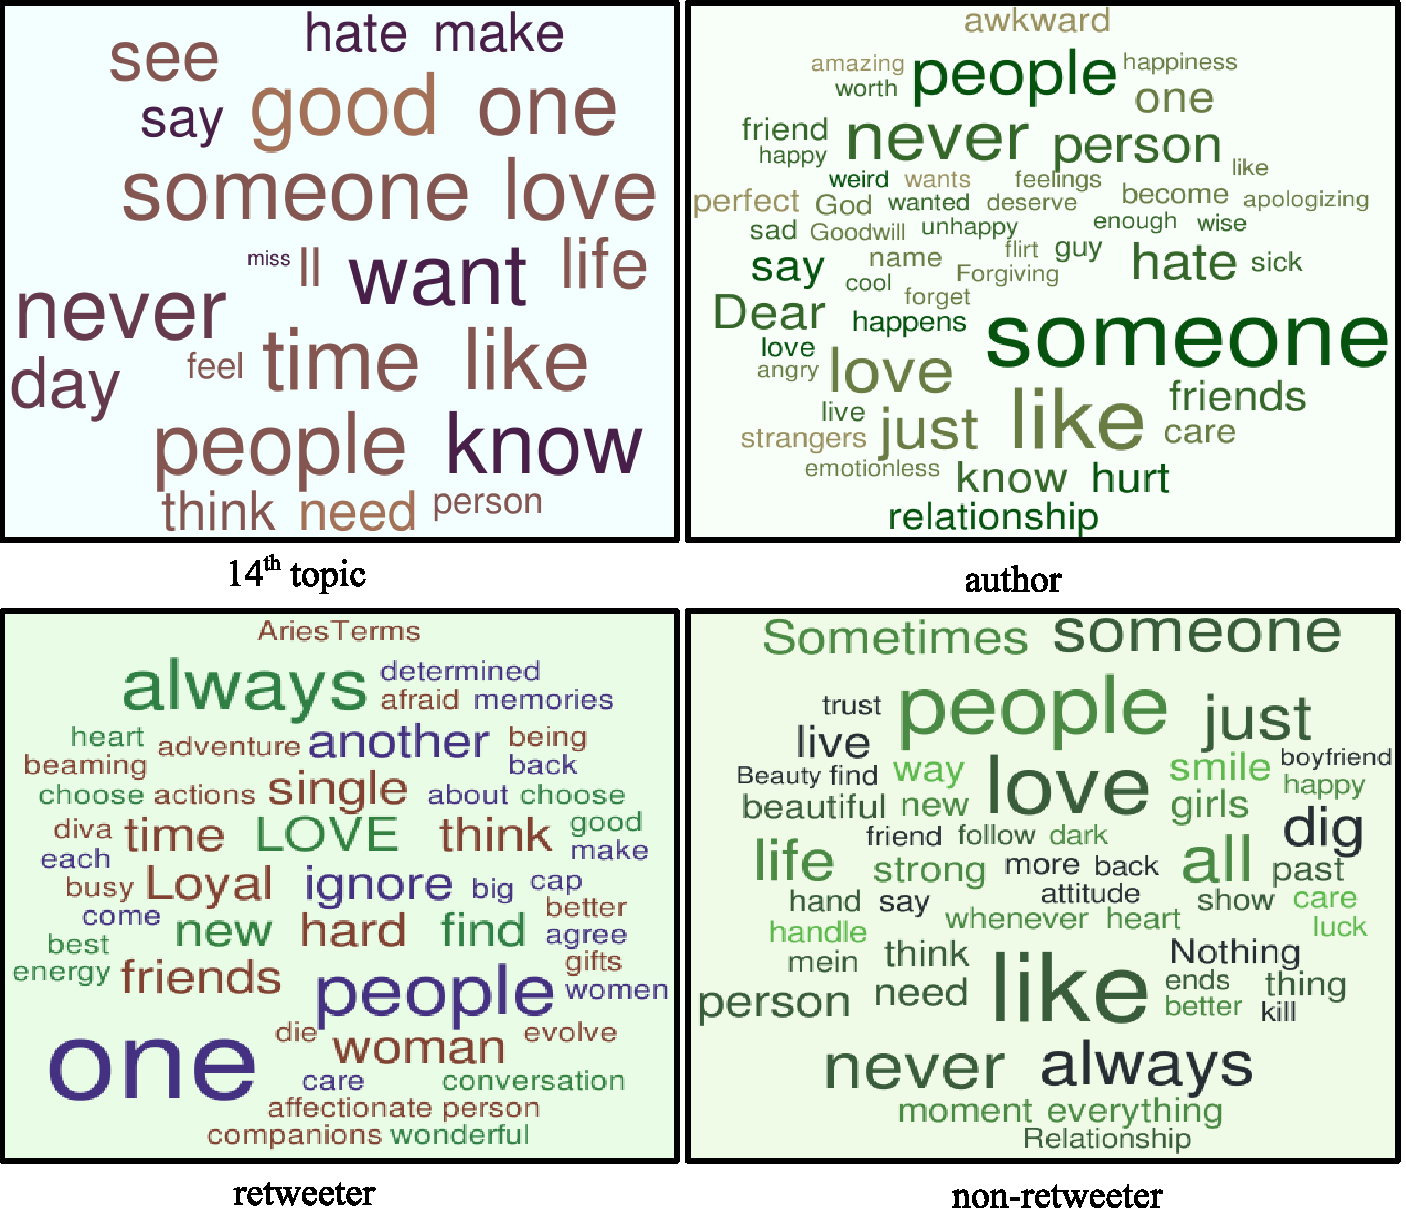
\includegraphics[height=320pt]{6-3.pdf}
\caption{$ 14^{th} $号话题、微博作者与两个关注者词云图}
\label{fig6-3}
\end{figure}

该微博谈论的是$ 14^{th} $号话题,话题是关于“love between people”,且作者对该话题的观点偏中性,可以看出这与图~\ref{fig6-2}中微博的主观模型以及图~\ref{fig6-3}中$ 14^{th} $号话题词云图是一致的;
微博作者有188条微博,主要集中在$ 14^{th} $号话题,观点分布为$O_{u_{a}}^{14} =( 0, 0.04, 0.05, 0.25, 0.35, 0.25, 0.05,  0.01 )$,偏中性;至于两个关注者,转发者有196条微博,主要涉及$ 14^{th} $号话题和$ 52^{nd} $号话题,话题分布比较均匀(其中$ w_{u_{r}}(14)=0.48 $),对$ 14^{th} $号话题,观点分布为$O_{u_{r}}^{14} =( 0, 0.02, 0.04, 0.15, 0.50, 0.13,  0.15,  0.01)$,偏中性;未转发者有156条微博,涉及到$ 14^{th} $号话题和$ 56^{th} $号话题,主要谈论了$ 14^{th} $号话题(其中$ w_{u_{n}}(14)=0.98 $),观点分布为$O_{u_{n}}^{14} =( 0, 0.01, 0.04, 0.10, 0.25, 0.45, 0.13, 0.02)$,偏正面。

表~\ref{tab6-4}是针对转发者和未转发者考虑三个引起转发因素计算的三个主观相似性,可以看出对于转发者来说,除了微博与其作者的主观相似性(度量微博流行性)外,其他两个主观相似性都明显高于未转发者。

\begin{table}[htp]
\centering
\caption{主观相似性比较}
\label{tab6-4}
\begin{tabular}{|c|c|c|c|}
\hline
相似性 & $ Sim(f,t) $ & $ Sim(f,u_a)  $ & $ Sim(u_a,t)  $\\
\hline
Retweeter & 0.854 & 0.967 & 0.886\\
\hline
Non-retweeter & 0.805 & 0.919 & 0.886\\
\hline
\end{tabular}
\end{table} 

从以上分析中看得出,对于微博的两个关注者,仅就感话题兴趣度来说,未转发者与微博以及微博作者更为相似(在共同话题$ 14^{th} $话题的兴趣度:作者$ w_{u_{a}}(14)=1.0 $,未转发者$ w_{u_{n}}(14)=0.98 $,转发者$ w_{u_{r}}(14)=0.48 $),但是考虑到主观相似性,转发者因为与微博以及作者有更相似的观点分布因而主观相似性更高(与微博主观相似性(度量吸引力)$ Sim(f,t)$:0.854 vs 0.805,与作者主观相似性(度量社交性)$ Sim(f,u_a)  $:0.967 vs 0.919),因此主观相似性的不同引发了他们不同的转发行为,从这个例子可以看出主观模型结合三个因素的主观相似性度量在解释用户转发行为上的作用。

\subsection{转发预测}
为了进一步定量的评价所提出的方法的有效性,分三阶段进行了转发预测实验。

首先,将本章模型与其他基于话题的模型进行对比实验。对比模型包括使用词袋模型对用户兴趣建模的TF-IDF模型、从用户产生内容中抽取实体对用户兴趣建模的基于实体模型(entity)以及使用用户微博中的hashtag的hashtag模型\upcite{Abel2011},对这些模型计算相似性的时候使用的是余弦相似性。

第二个阶段,将本章模型与两个话题情感生成模型(generative topic-sentiment models)TSM模型\upcite{Mei2007}以及JST模型\upcite{Lin2009}进行了对比实验。虽然TSM模型和JST模型也能同时对话题和话题相关的情感建模,但是他们的情感输出为正负二值极性。在训练这两个模型时,同样也是将用户所有微博作为一篇文档输入,并且使用本章定义的主观相似性计算方法~\ref{subsim}来计算三个主观相似性,但是在实际使用中是将三个相似性值组合起来作为特征同时加入到分类器中评价模型的预测性能。

第三个阶段,考虑到影响转发行为的其他因素,比如网络结构或用户Twitter使用习惯等元数据,也将本章模型和综合考虑其他因素的方法进行了对比。在此主要是和Luo\upcite{Luo2013}的工作(标记为“LUO”)进行了对比,表~\ref{tab6-5}是Luo\upcite{Luo2013}的模型使用的一些特征。
\begin{table}
\centering
\caption{LUO方法使用特征}
 \label{tab6-5}
  \begin{tabular*}{\textwidth}{@{\extracolsep{\fill}}| l l p{1.7in}|} 
 \hline 
\textbf{转发历史特征(RH)} & \textbf{取值范围} & \textbf{Description} \\
 \hline
  用户转发数目(Num\_fRu)& $N=\{0,1,2,...\}$ & 粉丝转发作者tweet的数目 \\
  用户提及数目(Num\_fMu)& $N=\{0,1,2,...\}$ & 粉丝提及作者tweet的数目 \\
  用户被转发数目(Num\_uRf)& $N=\{0,1,2,...\}$ & 作者转发粉丝tweet的数目 \\
  用户被提及数目(Num\_uMf)& $N=\{0,1,2,...\}$ & 作者提及粉丝tweet的数目 \\
  用户转发比例(Ratio\_retweet)& $[0,1]$ & 粉丝的tweet中转发tweet的比例 \\
  用户提及比例(Ratio\_mention)& $[0,1]$ & 粉丝的tweet中提及tweet的比例 \\
  \hline
 \hline
\textbf{用户特征(FS)} & \textbf{取值范围} & \textbf{Description} \\
 \hline
 发布tweet数目(Posts)  & $N^+=\{1,2,3,...\}$ & 作者以往发布tweet的数目 \\  
 粉丝数目(Followers) &$N=\{0,1,2,...\}$& 作者的粉丝数目 \\
 朋友数目(Friends)  & $N=\{0,1,2,...\}$ & 作者的朋友数目 \\
 分组数目(Listed)  &$N=\{0,1,2,...\}$& 作者的分组数目  \\
 验证用户(Verified)& $0$ or $1$ &  作者是否被官方验证\\
 \hline
 \hline
\textbf{用户活跃时间特征(FAT)} & \textbf{取值范围} & \textbf{Description} \\
 \hline
 时区时间(Timezone)& $0$ or $1$ &  粉丝是否与作者在同一个时区\\
 用户户活跃时间(PostTimeConsis)& $[0,1]$ & 粉丝发布tweet不同时间的数目比例 \\
\hline
 \hline
 \textbf{用户兴趣特征(FI)} & \textbf{取值范围} & \textbf{Description} \\
  相似兴趣(SimInterest)& $(-1,1)$ & tweet与粉丝以往发布tweet的相似度 \\
\hline
 \end{tabular*}
\end{table}
其中对用户兴趣建模部分,LUO方法使用的是简单的词袋模型,为了验证本章提出的方法在预测转发行为时的作用,实验将LUO方法中的用户兴趣特征替换为本章的三个主观相似性指标作为特征进行组合实验(使用“LUO+”前缀表示)。


实验中使用的是逻辑回归分类器(logistic regression classifier),用5倍交叉验证方式(5-fold cross-validation)训练测试,评价指标采用准确率。对于基准(baseline)设置,采用了一个基本的基准,该基准假设如果一个粉丝曾经转发目标微博作者的的微博,那么他很有可能会继续转发,因此直接将其预测为目标微博的转发者。
准确率结果如表~\ref{tab6-6}所示。

\begin{table}[htb]
\centering
\caption{准确率评测结果}
\label{tab6-6}
\begin{threeparttable}
\begin{tabular}{|l|l|l|l|}
\hline
特征 &准确率(\%) & 特征 &准确率(\%)\\
\hline
baseline & 60.85 & & \\
\hline
TF-IDF & 62.85   $\ast$ & LUO & 71.76 $ \ast  $\\
entity & 68.76  $\ast$ & LUO+entity & 72.15 $\ast$\\
hashtag & 59.12  & LUO+hashtag & 68.44 $\ast$\\
\hline
TSM & 67.44 $\ast$ & LUO+TSM & 68.23 $\ast$\\
JST & 68.13 $\ast$ & LUO+JST & 70.53 $\ast$\\
\hline
$ Sim(f,t) $ & 73.88   $\ast  \quad \ddagger $ &LUO+$ Sim(f,t)$ & 74.04  $ \ast \quad \ddagger $\\
$ Sim(f,u_a)  $ & 70.04   $\ast  $ & LUO+$ Sim(f,u_a)$ & 70.27  $ \ast $\\
$ Sim(u_a,t)  $ & 69.64   $\ast  $ & LUO+$ Sim(u_a,t)$ & 71.86  $ \ast $\\
$ sim_{all}  $ & \textbf{75.64}   $\ast \quad \ddagger $ & LUO+$ sim_{all}  $ & \textbf{78.15}  $ \ast \quad \ddagger $\\
\hline
\end{tabular}
\begin{tablenotes}
%  \centering
  \footnotesize
\item 显著性水平($p < 0.05$),使用$ \ast $标记性能显著超过基准,用$ \ddagger $标记性能显著超过LUO。
\end{tablenotes}
\end{threeparttable}
\end{table}
从表中可以看出:
\begin{itemize}
\item 首先,除了hashtag模型外,其他模型的准确率都显著超过了基准准确率(60.85\%),hashtag模型准确率为59.12\%,准确率低的主要原因是微博中hashtag的使用率过低而造成的数据稀疏。
\item 第二,对比实验中,两个主观相似性指标$ Sim(f,t) $和$ sim_{all}  $准确率显著超过了LUO方法(71.76\%),其中最高准确率为$ sim_{all}  $(75.64\%),是将三个主观相似性组合起来作为特征加入到分类器中,TF-IDF模型(62.85\%)仅仅比基准准确率稍好,entity模型(68.76\%)准确性接近 $ Sim(f,u_a)$(70.04\%)和$ Sim(u_a,t)  $(69.64\%),差别并不显著。
\item 第三,两个生成模型(TSM: 67.44\%,JST: 68.13\%)准确率不如本章提出的模型,主要原因在于他们的情感表示形式是二值极性表示,不能够很好的区分不同的观点,而我们的模型采用新的在情感空间的分布表示,可以区分用户细致的观点差别,从而可以对用户转发行为的主观动机建模。
\item 最后,在组合实验中,$ Sim(f,t) $指标对准确率的提高显著(LUO+$ Sim(f,t) $,准确率提高2.12\%),但是其他两个主观相似性以及entity模型加入后准确率提高不明显,加入hashtag和两个生成模型后准确率反而会降低,值得注意的是将三个主观相似性同时加入到LUO方法中准确率提高最多(LUO+$ sim_{all}  $,准确率提高6.39\%)。
\end{itemize}

综上所述,转发预测结果显示主观模型以及考虑三个因素的主观相似性可以很好的预测用户的转发行为,能够作为分析转发行为的有效途径。

\section{小结}
本章在第五章提出的主观模型基础上从主观动机角度对用户的转发行为的进行了分析,提出了新的主观相似性计算方法,并通过考虑影响用户转发行为的微博吸引力、朋友间的社交性以及微博的流行性三个不同因素,对用户的转发行为进行分析,并将三个因素量化为三个主观相似性。实验结果证明了主观相似性与转发行为存在相关性,可以很好的解释和预测用户的转发行为,对于理解用户的转发行为的主观动机有重要作用。


\chapter{总结与展望}
\label{con}
社交媒体已经逐步发展完善,随着用户使用社交媒体的普及,带有用户观点信息的文本数据正以指数级速度增长,本文主要围绕社交媒体中观点信息的挖掘、分析以及在转发行为分析中的应用展开研究。通过情感词典资源的建设、情感极性分类以及利用情感分析结果对社交媒体用户的主观性建模和应用等任务,本文充分利用了社交媒体作为媒体所产生文本的语言特点和社交媒体用户之间广泛连接的社交功能来帮助解决这些问题。

对社交媒体文本数据中的观点信息分析研究能够从社交媒体海量数据中发现有借鉴意义的信息,无论对于其他研究还是商业应用都有价值。为了确定观点信息需要从文本中抽取分离出能够识别用户看法、态度、立场以及情感的表达方式,本文特别针对社交媒体的文本进行了情感知识词典的构建和对社交媒体非规范化文本的情感分类研究,因此可以从社交媒体中挖掘分析观点信息。
在获得文本中的观点信息后,可以利用这些观点信息来认识作为社交媒体使用主体的用户,对用户在社交媒体上表达的观点进行集成分析,对用户的主观性进行建模。得到的主观模型可以对于理解用户的在线行为提供帮助。

\section{工作总结}

本文的主要工作可以从以下五个方面来总结:

首先,针对现有中文情感词典相对较少并且缺乏可靠性问题,提出了借鉴现有的丰富的英文情感词典资源进行跨语言的情感知识转化研究。为了更准确的反映词语的情感情感极性值,本文结合中文语义知识库HowNet,将知识库中的语义关系融合进词语的情感值计算过程中,利用HowNet的义原与词语的中英文对应关系将英文情感词典SentiWordnet的情感知识转化为中文词语的情感知识,形成中文情感词典SentiHowNet。

第二,仅仅依靠从词典资源标注或转化的情感知识识别文本的观点信息会受到词典覆盖面以及领域适应性的限制,而且社交媒体语言的动态性决定需要一种能够及时从社交媒体语料数据中发现新的情感词并扩展情感词典的方法,本文通过研究中文的连词语言规则和上下文统计特征,以实验验证了三种从语料中抽取词语并计算情感值的情感词典扩展方法,使得情感词典可以适应社交媒体语言不断增长与变化的特点。

第三,从社交媒体文本一般是不规范的短文本,从中确定观点信息需要对这种不规范短文本的情感倾向性进行分类,本文通过将情感分类问题形式化为特殊的文本分类问题,根据词语在表达情感极性时的不同作用,提出了特征空间划分假设,将情感分类的词语特征空间划分为领域独立和领域依赖两部分,并使用现成的无须标注成语资源和远监督方式在不同的特征空间训练通用的分类器和微博情感分类器,将两个分类器用一个自举式机器学习框架组合在一起形成一个更强情感分类器,本文提出的方法在缺少大规模的标注文本而无法训练分类器的情况下,使用无监督方式达到了有监督机器学习方法的性能。

第四,用户在使用社交媒体时发表的文本一般是短小的、碎片化的,因此用户的观点信息散布在这些碎片化的文本信息中,目前情感分析研究主要是针对文本片段分析抽取其中的观点信息,无法完整呈现出一个用户整体的观点,因此本文提出了用户观点集成问题,并就这一问题提出了主观模型的概念,主观模型可以将用户在社交媒体中感兴趣的话题以及针对这些话题的发表的观点进行集成,并使用一种通用的细粒度的形式表示观点,将观点表示为在可扩展情感表示空间的一种概率分布,主观模型可以对用户在社交媒体中的整体观点信息集成表示,解决了用户信息的碎片化而造成的观点表示不全面不准确问题。

最后,针对信息传播研究中被忽略的用户的传播主观动机问题,结合主观模型对用户的主观性建模分析,本文主要分析了Twitter中用户在信息传播中的转发行为,将用户转发行为的主观动机量化为用户之间以及用户与微博之间的主观相似性,通过分析影响用户转发行为的三个因素,也就是微博内容上的吸引力,朋友间的社交需求以及微博信息的流行性,将其转化为三个主观相似性度量值,并分析研究了它们与用户转发行为之间的关系,在真实Twitter数据集上的实验证明了主观相似性度量与转发行为的相关性,以及在预测转发行为的有效性。

\section{工作展望}
展望未来,社交媒体中的观点信息的分析研究及其相关应用还有很多工作需要完成。在此总结以下亟待探索的研究方向和路线:
  \begin{enumerate}
  \item 以Twitter为代表的社交媒体一个重要特点就是信息的实时性,目前虽然有一些研究工作,但主要都是围绕在Twitter中发现实时客观信息展开,包括新事件发现\upcite{petrovic2010streaming,becker2011beyond,weng2011event,naaman2011hip,benson2011event,petrovic2012using,kanhabua2013understanding}、实时灾害报道(如地震、疾病、火灾等)\upcite{sakaki2010earthquake,paul2011you,aramaki2011twitter,abel2012twitcident,yin2012esa}等,在TREC评测中的Twitter检索\upcite{efron2011estimation,metzler2012structured,zhang2012query,soboroff2012evaluating,choi2012temporal,amati2012survival,miyanishi2013combining}也将实时性作为一个重要指标。本文的研究中,并未对观点信息挖掘与分析受到实时性的影响进行讨论研究,社交媒体语言的实时性特点需要后续工作中考虑到相关研究\upcite{Das2014,Guerra2014}。
  
 \item 本文的社交媒体中观点信息的研究还是对比较常用的几个类型(比如评论和微博)进行的研究,实际上社交媒体还有很多类型,如Facebook\footnote{\url{https://www.facebook.com/}}、YouTube\footnote{\url{https://www.youtube.com/}}、 Flickr\footnote{\url{https://www.flickr.com/}}等等。这些社交媒体肯定都有自己独特的特点,在这些类型社交媒体数据上进行观点的挖掘与分析需要研究其独特的情感表达方式;另外,多种社交媒体综合和跨媒体的信息交互与传播也会对观点信息的分析提出新课题,这就需要研究者在充分理解各种社交媒体的特点和用户对各种社交媒体不同使用习惯上,提出方法解决问题。
 
 \item 目前将观点分析研究结合与其他应用和任务相结合是一个新的研究方向,主要是原因是越来越多的应用和任务需要以社交媒体用户观点信息作为有用的特征使用,比如在股市指数的预测中,用户的观点指标会影响人的投资意愿\upcite{bollen2011twitter,Antweiler2004,Zhang2011},未来工作重点将结合更多实际任务或应用有针对性的进行观点信息的分析。
  \end{enumerate}
  
总之,针对社交媒体中的观点信息的研究还有许多问题等待着去解决,我们将继续深入研究相关问题。

\newpage 
\mbox{} 
\newpage

%%% Local Variables:
%%% mode: latex
%%% TeX-master: "../main"
%%% End:

\begin{ack}
“Learning is more imortant than knowing”,尤其是对于工作过一段时间的人来说,在感知到自己所知甚少时候能有机会重新学习,进行课题研究,需要感谢的人实在是太多。

首先感谢我的导师王挺教授,从一开始能够接受一名在职的考博学生,您就以开放而又严谨的治学态度给予我最大的支持,感谢您在过去的五年中精细的学术指导和研究建议,您在学术领域的专业深度和开阔视野激发了我在文本信息处理研究的巨大兴趣,感谢您让我拥有充分的研究自由,培养了我深入思考和独立解决问题的能力,这些都对于我顺利完成博士课题研究都是必不可少的。

感谢课题组的唐晋韬、周云、李岩、麻大顺、刘培磊、岳大鹏、刘海池、汝承森、张文文、姜仁会、胡长龙、李欣奕,和大家一起亦师亦友共同探讨自然语言处理领域最前沿的问题让我获益非浅,在艰辛的求学到路上大家互相帮助,苦中作乐的日子让我重新体会到了无私的同学友谊。

感谢计算机学院的学院领导在工作、考博和学习期间给我的关怀和指导;感谢学员大队的同事,在我求学阶段给我指导、鼓励还有协助;感谢博士队队领导和各位博士战友,在一起“共同战斗”的日子永远值得回味。

最后,也是做重要的,感谢我的家人,没有家人的支持就没有我顺利的博士学习研究:感谢我的妻子黄丽达,感谢你牺牲自己的工作学习对我的支持;感谢我五岁的女儿,你的出生给我生活带来无尽的乐趣;感谢我的岳父母,在我读博期间对我们这个小家的生活上无微不至的照顾;感谢在山东的父母,远在千里你们的关爱依然!
\end{ack}
\newpage 
\mbox{} 
\newpage

\cleardoublepage
\phantomsection
\addcontentsline{toc}{chapter}{参考文献}
\bibliographystyle{bstutf8}
\bibliography{ref/refs}

\begin{resume}

  \section*{发表的学术论文} % 发表的和录用的合在一起

  \begin{enumerate}[{[}1{]}]
  \addtolength{\itemsep}{-.36\baselineskip}%缩小条目之间的间距,下面类似
  
  \item Zhunchen Luo, Miles Osborne, Sasa Petrovic and Ting Wang. Improving Twitter Retrieval by Exploiting Structural Information. In {\it Proceedings of the Twenty-Sixth AAAI Conference on Artificial Intelligence} (\textbf{AAAI 2012}), Toronto, Canada, July 2012. \textbf{(CCF A类会议,人工智能领域顶级会议)}
 
 \item Zhunchen Luo, Miles Osborne, Jintao Tang and Ting Wang. Who Will Retweet Me? Finding Retweeters in Twitter. In {\it Proceedings of the Thirty-Sixth International ACM SIGIR Conference on Research and Development in Information Retrieval} (\textbf{SIGIR 2013}), Dublin, Ireland, July 2013.\textbf{(CCF A类会议,信息检索领域顶级会议,获得会议旅行奖金1300美元)}

\item Zhunchen Luo, Miles Osborne and Ting Wang. Opinion Retrieval in Twitter. In {\it Proceedings of the Sixth International AAAI Conference on Weblogs and Social Media} (\textbf{AAAI-ICWSM 2012}), Dublin, Ireland, June 2012. \textbf{(社交媒体领域顶级会议,获得会议旅行奖金300美元)}

 \item  Zhunchen Luo, Miles Osborne and Ting Wang. An Effective Approach to Tweets Opinion Retrieval. To appear in \textbf{World Wide Web Journal}. (\textbf{SCI期刊,影响因子1.196})
 
 \item Zhunchen Luo, Jintao Tang and Ting Wang. Propagated Opinion Retrieval in Twitter. In {\it Proceedings of the Fourteenth International Conference on Web Information System Engineering} (\textbf{WISE 2013}), Nanjing, China, October 2013.\textbf{(CCF C类会议,信息检索与数据挖掘领域重要会议)}

\item Zhunchen Luo, Jintao Tang and Ting Wang. Improving Keyphrase Extraction from Web News by Exploiting Comments Information. In {\it Proceedings of the Fifteenth International Asia-Pacific Web Conference} (\textbf{APWeb 2013}), Sydney, Australia, April 2013. \textbf{(CCF C类会议,信息检索与数据挖掘领域重要会议)}

\item Zhunchen Luo, Lan Rao, Chengsen Ru and Ting Wang. Finding High-Quality Posts from Microblogging Conversations. In {\it the Eighth International Conference on Modeling Decisions for Artificial Intelligence (\textbf{MDAI 2011})}, Changsha, China, July, 2011.

\item 罗准辰,王挺. 基于分离模型的中文关键词提取算法研究. 中文信息学报, 2009,23 (01): 63-70.

\item 罗准辰,王挺. 搜索词同现网络研究. 第六届全国信息检索学术会议(\textbf{CCIR 2010}),镜泊湖,2010年8月.

  \end{enumerate}

\end{resume}

% 最后,需要的话还要生成附录,全文随之结束。
\appendix
\backmatter
%% TeX
\chapter{模板提供的希腊字母命令列表}

大写希腊字母:
\begin{table}[htbp]
\centering
\begin{tabular}{llll}
\toprule
$\Gamma$~\verb|\Gamma| & $\Lambda$~\verb|\Lambda| & $\Sigma$~\verb|\Sigma| & $\Psi$~\verb|\Psi| \\
$\Delta$~\verb|\Delta| & $\Xi$~\verb|\Xi| & $\Upsilon$~\verb|\Upsilon| & $\Omega$~\verb|\Omega| \\
$\Theta$~\verb|\Theta| & $\Pi$~\verb|\Pi| & $\Phi$~\verb|\Phi| & \\
\midrule
$\varGamma$~\verb|\varGamma| & $\varLambda$~\verb|\varLambda| & $\varSigma$~\verb|\varSigma| & $\varPsi$~\verb|\varPsi| \\
$\varDelta$~\verb|\varDelta| & $\varXi$~\verb|\varXi| & $\varUpsilon$~\verb|\varUpsilon| & $\varOmega$~\verb|\varOmega| \\
$\varTheta$~\verb|\varTheta| & $\varPi$~\verb|\varPi| & $\varPhi$~\verb|\varPhi| & \\
\bottomrule
\end{tabular}
\end{table}

小写希腊字母:
\begin{table}[htbp]
\centering
\begin{tabular}{llll}
\toprule
$\alpha$~\verb|\alpha| & $\theta$~\verb|\theta| & $o$~\verb|o| & $\tau$~\verb|\tau| \\ 
$\beta$~\verb|\beta| & $\vartheta$~\verb|\vartheta| & $\pi$~\verb|\pi| & $\upsilon$~\verb|\upsilon| \\ 
$\gamma$~\verb|\gamma| & $\iota$~\verb|\iota| & $\varpi$~\verb|\varpi| & $\phi$~\verb|\phi| \\ 
$\delta$~\verb|\delta| & $\kappa$~\verb|\kappa| & $\rho$~\verb|\rho| & $\varphi$~\verb|\varphi| \\ 
$\epsilon$~\verb|\epsilon| & $\lambda$~\verb|\lambda| & $\varrho$~\verb|\varrho| & $\chi$~\verb|\chi| \\ 
$\varepsilon$~\verb|\varepsilon| & $\mu$~\verb|\mu| & $\sigma$~\verb|\sigma| & $\psi$~\verb|\psi| \\ 
$\zeta$~\verb|\zeta| & $\nu$~\verb|\nu| & $\varsigma$~\verb|\varsigma| & $\omega$~\verb|\omega| \\ 
$\eta$~\verb|\eta| & $\xi$~\verb|\xi| & $\varkappa$~\verb|\varkappa| & $\digamma$~\verb|\digamma| \\ 
\midrule
$\upalpha$~\verb|\upalpha| & $\uptheta$~\verb|\uptheta| & $\mathrm{o}$~\verb|\mathrm{o}| & $\uptau$~\verb|\uptau| \\ 
$\upbeta$~\verb|\upbeta| & $\upvartheta$~\verb|\upvartheta| & $\uppi$~\verb|\uppi| & $\upupsilon$~\verb|\upupsilon| \\ 
$\upgamma$~\verb|\upgamma| & $\upiota$~\verb|\upiota| & $\upvarpi$~\verb|\upvarpi| & $\upphi$~\verb|\upphi| \\ 
$\updelta$~\verb|\updelta| & $\upkappa$~\verb|\upkappa| & $\uprho$~\verb|\uprho| & $\upvarphi$~\verb|\upvarphi| \\ 
$\upepsilon$~\verb|\upepsilon| & $\uplambda$~\verb|\uplambda| & $\upvarrho$~\verb|\upvarrho| & $\upchi$~\verb|\upchi| \\ 
$\upvarepsilon$~\verb|\upvarepsilon| & $\upmu$~\verb|\upmu| & $\upsigma$~\verb|\upsigma| & $\uppsi$~\verb|\uppsi| \\ 
$\upzeta$~\verb|\upzeta| & $\upnu$~\verb|\upnu| & $\upvarsigma$~\verb|\upvarsigma| & $\upomega$~\verb|\upomega| \\ 
$\upeta$~\verb|\upeta| & $\upxi$~\verb|\upxi| & & \\ 
\bottomrule
\end{tabular}
\end{table}

希腊字母属于数学符号类别,请用\verb|\bm|命令加粗,其余向量、矩阵可用\verb|\mathbf|。


\end{document}
